	% ===============================================
% Sogenannte Praeambel: Seiteneinstellungen etc.
% ===============================================

\documentclass[german,10pt,oneside, fleqn, a4paper]{article}

%%% Eingebundene Pakete: werden hier nicht alle gebraucht, schaden aber auch nicht.
\usepackage{hyperref}
\usepackage{graphicx}
\graphicspath{}
\usepackage{pdfpages}
\usepackage[german]{babel}
\usepackage{amsmath,amsthm,amssymb,amsfonts,amscd,amsbsy,amsxtra}
\usepackage{epsfig,color}
\usepackage{wrapfig}
\usepackage{listings}
\usepackage{fancyheadings}
\usepackage{psfrag}
\usepackage{extarrows}
\usepackage{amsmath}
\usepackage{float}
\usepackage{enumerate}
\usepackage{enumitem}
\usepackage[T1]{fontenc} 
\usepackage{ucs}
\usepackage[utf8]{inputenc}
\usepackage[font=scriptsize]{caption}

\usepackage{marvosym}
\let\marvosymLightning\Lightning


\usepackage{mathtools}



\usepackage{scalerel,stackengine}
\stackMath
\newcommand\reallywidehat[1]{%
\savestack{\tmpbox}{\stretchto{%
  \scaleto{%
    \scalerel*[\widthof{\ensuremath{#1}}]{\kern-.6pt\bigwedge\kern-.6pt}%
    {\rule[-\textheight/2]{1ex}{\textheight}}%WIDTH-LIMITED BIG WEDGE
  }{\textheight}% 
}{0.5ex}}%
\stackon[1pt]{#1}{\tmpbox}%
}
\parskip 1ex



%%% Neudefinition von Kommandos, um sich Tipp-Arbeit zu ersparen 
\newcommand{\tscheb}{Tschebyscheff}	 
\newcommand {\Q}	{\mathbb{Q}}
\newcommand {\R}	{\mathbb{R}}
\newcommand {\N}	{\mathbb{N}}
\newcommand {\C}	{\mathbb{C}}
\newcommand{\Ra}	{\Rightarrow}
\newcommand{\La}	{\Leftarrow}
\newcommand{\LRa}{\Leftrightarrow}
\newcommand{\ra}{\rightarrow}

%%% Veraenderung des Seitenlayouts
%\setlength{\oddsidemargin}{-1cm}
%\setlength{\evensidemargin}{0cm}
%\setlength{\textwidth}{18cm}
%\setlength{\textheight}{26cm}
%\setlength{\parindent}{0pt}
%\setlength{\topmargin}{-2cm}
%\pagestyle{empty}

\sloppy



%MACROS!!!
\newcommand{\verteq}{\rotatebox{90}{$\,=$}}
\newcommand{\equalto}[2]{\underset{\scriptstyle\overset{\mkern4mu\verteq}{#2}}{#1}}
\newcommand{\lsup}[1][n]{\limsup\limits_{#1\rightarrow\infty}}
\newcommand{\linf}[1][n]{\liminf\limits_{#1\rightarrow\infty}}
\newcommand{\sm}[2][\infty]{\sum\limits_{#2}^{#1}}
\newcommand{\brc}[1]{\left(#1\right)}
\newcommand{\brac}[1]{\left\lbrace #1\right\rbrace}
\newcommand{\CUP}[2][\infty]{\bigcup\limits_{#2}^{#1}}
\newcommand{\CAP}[2][\infty]{\bigcap\limits_{#2}^{#1}}
\newcommand{\folge}[3][\N]{\left(#2_#3\right)_{#3\in #1}}
\newcommand{\norm}[1]{\left\Vert #1 \right\Vert}
%\newcommand{\myeq}[2][=]{\mathrel{\overset{\makebox[0pt]{\mbox{\normalfont\small\sffamily #2}}}{#1}}}
\newcommand{\myeq}[2][=]{\stackrel{\mathclap{\normalfont\tiny\mbox{#2}}}{#1}}
\newcommand{\QED}{\begin{flushright}$\qed$\end{flushright}}
\newcommand{\mat}[1]{\begin{pmatrix}#1\end{pmatrix}}
\newcommand{\mc}[1]{\mathcal{#1}}
\newcommand{\lp}[1]{\mc{L}^{#1}}
\newcommand{\la}{\lp{1}}
\newcommand{\beweis}{\textbf{Beweis}\\}
\newcommand{\toinf}{\rightarrow\infty}
\newcommand{\fn}[1][n]{\ \forall #1\in\N}
\newcommand{\1}[1]{1_{#1}}
\newcommand{\2}[1]{\1{\brac{#1}}}
\newcommand{\xnorm}{\norm{X_n-X}}
\newcommand{\xr}[2][]{\xrightarrow[#1]{#2}}
\newcommand{\cb}[1][d]{\mc{C}_b\brc{\R^{#1}}}
\newcommand{\rbor}[1][d]{\brc{\R^{#1},\mc{B}\brc{\R^{#1}}}}
\newcommand{\raum}{\brc{\Omega,\mc{F},P}}
\newcommand{\rraum}{\brc{\Omega,\mc{F},\mc{P}}}
\newcommand{\inv}{^\leftarrow}
\newcommand{\fe}{\forall\varepsilon>0}
\newcommand{\xn}{x_n}
\newcommand{\Xn}{X_n}
\newcommand{\intr}{\int\limits_\R}
\newcommand{\wid}{\text{\marvosymLightning}}
\newcommand{\nn}{n\in\N}
\newcommand{\g}{\mc{G}}
\newcommand{\f}{\mc{F}}
\newcommand{\p}{\mc{P}}
\newcommand{\h}{\mc{H}}
\newcommand{\uu}{\mc{U}}
\newcommand{\sumi}{\sm[n]{i=1}}
\newcommand{\qf}{\quad\forall}
\newcommand{\stuff}{{\otimes n}}
\DeclareMathOperator*{\kreuz}{\otimes}
\newcommand{\kreuzi}{\kreuz\limits_{i=1}^n}
% ==============================================
% Start des eigentlichen Dokumentes
% ==============================================
\begin{document}



    
\vspace{0.5cm}
\begin{center}
{\bf \Large Stochastik } \\[2ex]
\end{center} 
\tableofcontents
\pagebreak




\marginpar{1. Vorlesung 16.04.2018}
\part{Grundlagen der Maßtheorethischen Wahrscheinlichkeitstheorie}



\section{0-1 Gesetze}
Gegeben sei ein Wahrscheinlichkeitsraum $\raum$.\\

\subsection{Definition (liminf,limsup)}
Sei $(A_n)_{n\in\N}$ eine Folge in $\f$. Dann definiert man 
\begin{list}{}{}
\item \(\limsup\limits_{n\rightarrow \infty}A_n=\bigcap\limits_{n=1}^\infty\bigcup\limits_{m=n}^\infty A_m=\lbrace w\in \Omega:w \in A_n\ \infty\text{ -oft}\rbrace\) \\ 
\glqq Unendlich viele der Ereignisse $A_n$ treten ein \grqq.
\item \(\liminf\limits_{n\rightarrow\infty}A_n=\bigcup\limits_{n=1}^\infty\bigcap\limits_{m=n}^\infty A_m=\lbrace w\in \Omega:w \in A_n\text{für schließlich alle n}\rbrace\) \\
\glqq Bis auf endlich viele treten alle der Ereignisse $A_n$ ein \grqq.
\end{list}

\subsection{Bemerkung}
$\liminf\limits_{n\rightarrow\infty}A_n\subseteq \limsup\limits_{n\rightarrow\infty}A_n$

\subsection{Lemma (Borel-Cantelli)}
Sei $(A_n)_{n\in\N}$ eine Folge in $\f$. 
\begin{list}{}{}
\item $\sum\limits_{n=1}^\infty P(A_n) < \infty\Rightarrow P(\limsup\limits_{n\rightarrow\infty}A_n)=0$
\item Ist $(A_n)_{n\in\N}$ zusätzlich Unabhängig, so gilt $\sum\limits_{n=1}^\infty P(A_n) = +\infty\Leftrightarrow P(\limsup\limits_{n\rightarrow\infty}A_n)=1$
\end{list}

\textbf{Beweis}\\
Es gilt: $P \left(\bigcup\limits_{i=1}^\infty A_i\right) \leq \sum\limits_{i=1}^\infty P(A_i)$\begin{enumerate}[label=(\alph*)]
\item $\forall \varepsilon>0\ \exists N\in\N$ mit\\
$P\left(\limsup\limits_{n\rightarrow\infty}A_n\right)\leq P\left(\bigcup\limits_{m=N}^\infty A_m \right) \leq \sum\limits_{m=N}^\infty P(A_m) \leq \varepsilon$
\item \glqq $\Rightarrow$\grqq:\\
Es gilt $\forall\alpha>0:\ 1-\alpha\leq e^{-\alpha}$ und\\
 $\left(\limsup\limits_{n\rightarrow\infty}A_n\right)^c=\liminf\limits_{n\rightarrow\infty}A_n^c=\bigcup\limits_{n=1}^\infty\bigcap\limits_{m=n}^\infty A_m^c$\\
$P\left(\bigcap\limits_{m=n}^\infty A_m^c\right)=\prod\limits_{m=n}^\infty\left(1-P(A_m)\right)$ wegen Unabhängigkeit und Monotonie. Somit folgt\\
$P((\limsup\limits_{n\rightarrow\infty}A_n)^c)
\leq\sum\limits_{n=1}^\infty P\left(\bigcap\limits_{m=n}^\infty A_m^c\right)
=\sum\limits_{n=1}^\infty\prod\limits_{m=n}^\infty (1-P(A_m))
\leq\sum\limits_{n=1}^m\prod\limits_{m=n}^\infty e^{-P(A_m)}
=\sum\limits_{n=1}^\infty \underbrace{e^{-\overbrace{\sum\limits_{m=n}^\infty P(A_m)}^{\infty}}}_{0}=0$\\\\
\glqq $\Leftarrow$\grqq:$\sum\limits_{n=1}^\infty P(A_n)<\infty$ wäre ein Widerspruch zu a)  \QED
\end{enumerate}

$\limsup , \liminf$ sind Beispiele \textit{Terminaler Ereignise}.





\marginpar{2. Vorlesung 17.04.2018}

\subsection{Definition (Terminale Ereignisse)}
Seien $(\f_n)_{n\in\N}\subset F$ $\sigma$-Algebren und $T_n=\sigma\left(\bigcup\limits_{m=n}^\infty\f_m\right)$. \\
Dann heißt $T_\infty:=\bigcap\limits_{n=1}^\infty\f_n$\\ terminale $\sigma$-Algebra $(\sigma$-Algebra der Terminalen Ereignisse$)$. \\
Terminale Ereignisse hängen nicht von den ersten Endlich vielen $\f_n$ ab.

\subsection{Beispiel}
Sei $(A_n)_{n\in\N}\in F$. Setze $F_n=\lbrace p,\Omega,A_n,A_n^c\rbrace.$\\
Dann gilt \[\bigcup\limits_{m=n+i}^\infty A_m\in T_n$ $\forall n\in\N, i\in\N_0\].
Somit \[\bigcap\limits_{n=1}^\infty\bigcup\limits_{m=n}^\infty A_m \in T_n \forall n \in \N \Rightarrow\limsup\limits_{n\rightarrow\infty}A_n\in T_\infty\].\\
Da $T_\infty$ $\sigma$-Algebra, gilt auch\\
\[\liminf\limits_{n\rightarrow\infty}A_n=\left(\limsup\limits_{n\rightarrow\infty}A_n^c\right)^c\in T_\infty\]

\subsection{Definition (Unabhängige Mengensysteme)}
Sei $\raum$ ein Wahrscheinlichkeitsraum und $I\neq\emptyset$ eine Indexmenge. Eine Familie von Mengensystemen $\left(\varphi_n\right)_{n\in\N}$ mit $\varphi_i \subseteq\f$  heißt unabhängig, falls $\forall y\subseteq I, \vert y \vert < \infty, y\neq\emptyset$ gilt \\
\[P\left(\bigcap\limits_{j\in J}A_j\right)=\prod\limits_{j\in J}P\left(A_j\right)$ $\forall A_j \in\varphi_j\]\\
 \textbf{Beachte}: Sei $\left( x_i \right)_{i\in I}$ eine Familie von Zufallsvariablen mit $x_i\raum\mapsto\left(\Omega_i,\f_i \right)$, dann sind diese Unabhängig genau dann, wenn die Familie von $\sigma$-Algebren $\left(x_i^{-1}\left(\f_i\right)\right)_{i\in I}$ unabhängig ist.

\subsection{Satz (0-1 Gesetze von Kolmogorov)}
Sei $\left(\f_n\right)_{n\in\N}$ eine Folge unabhängiger $\sigma$-Algebren, $\f_n\subseteq\f$. Dann gilt\\
\[P\left(A\right)\in \lbrace 0,1\rbrace\ \forall A \in T_\infty\] \\

\textbf{Beweis:}\\
Für $A\in T_\infty$ setze $\mc{D}=\lbrace P\in\sigma\left(\bigcup\limits_{n=1}^\infty F_n\right):\text{ P ist unabhängig von }A\rbrace$. Es genügt zu zeigen: $T_\infty\subseteq \mc{D}$. Dann ist $A$ unabhängig von $A$, und somit $P(A)=P(A\cap A)=P(A)^2$ und somit $P(A)\in\lbrace 0,1 \rbrace$.\\
Es gilt: $T_{n+1}$ und $G_n:=\sigma(\bigcup\limits_{i=1}^n\f_i)$ sind unabhängig.\\
Da $A\in T_{n+1}$ folgt $G_n\subseteq \mc{D}\ \forall n\in\N\Rightarrow G_0:=\bigcup\limits_{n=1}^\infty G_n\subseteq \mc{D}$. Wegen $G_n\subseteq G_{n+1}$ ist $G_0$ $\cap$-stabil. Mit dem Eindeutigkeitssatz für Maße sind folglich\\
    $\vartheta:\sigma(G_0)\rightarrow\R^+,\ \ G\mapsto P(G\cap A)$\\
    $\mu:\sigma(G_0)\rightarrow\R^+,\ \ G\mapsto P(G)P(A)$ identische Maße.
$\Rightarrow\sigma(G_0)\subseteq \mc{D}$.
Offensichtlich gilt $T_n\subseteq\sigma(G_0)\ \forall n\in\N$\\
$\Rightarrow T_\infty\subseteq\sigma(G_0)\subseteq \mc{D}$.\QED	

\subsection{Korollar}
Sei $\left(A_n\right)_{n\in\N}$ eine Folge unabhängiger Ereignisse. Dann gilt
\[P\left(\limsup\limits_{n\rightarrow\infty}A_n\right)\in\lbrace 0,1\rbrace\]

\subsection{Korollar}
Sei $X:\left(\Omega,\f\right)\rightarrow\left(\bar\R,B\left(\bar\R\right)\right)$ eine $T_\infty$-Messbare Zufallsvariable. Dann gibt es eine Konstante $c\in\R$ mit $P\left(X=c\right)=1$.\\\\
\textbf{Beweis}\\
$A_q:=\lbrace X\leq q\rbrace\in T_\infty\ \forall q\in \Q\Rightarrow P(A_q)\in\lbrace 0,1\rbrace$ und $P(A-q)$ monoton wachsend in $q$. Setze $c:=\inf\lbrace q\in\Q:P(A_q)=1\rbrace$. Dann folgt \\
$P(X<c)=P(\bigcup\limits_{\substack{q<c\\q\in\Q}}A_q)=0$\\
$P(X>c)=P(\bigcup\limits_{\substack{q>c\\q\in\Q}}A_q)=0$\\$\Rightarrow P(X=c)=1$\QED

\subsection{Beispiel}
Sei $\left(X_n\right)_{n\in\N}$ eine Folge reeller Zufallsvariablen und $\alpha \searrow_{n\rightarrow\infty}0$. Dann gilt:
\[ P\left(\underbrace{\lbrace\omega:\lim\limits_{N\rightarrow\infty} \alpha_N\sum\limits_{i=1}^NX_i\left(\omega\right)=0\rbrace}_{=:A}\right)\in\lbrace 0,1 \rbrace\]

\textbf{Beweis}\\
Sei $\f_n=X_n^{-1}(B(\R))$. Dann ist $(\f_n)_{n\in\N}$ eine unabhängige Folge von $\sigma$-Algebren.\\
$\alpha_N\sum\limits_{i=1}^\infty X_i=\underbrace{{\alpha_N}\sum\limits_{i=1}^n X_i}_{\xrightarrow[N\rightarrow\infty]{}0}+\underbrace{{\alpha_N}\sum\limits_{i=n+1}^\infty X_i}_{\sigma_{n+1}-messbar}\ \ \forall n\in\N$\\
$A=\bigcap\limits_{n=1}^\infty\underbrace{\lbrace\alpha_N\sum\limits_{i=n}^NX_i\xrightarrow[N\rightarrow\infty]{}0\rbrace}_{\in T_n}\in T_\infty$\QED
Inbesondere gilt:\\
$P(\lbrace\lim\limits_{n\rightarrow\infty}\dfrac{1}{n}\sum\limits_{i=1}^n(X_i-E(X_i))=0\rbrace)\in\lbrace 0,1\rbrace$\\
für alle unabhängigen Folgen von Zufallsvariablen mit endlichem Erwartungswert, das heißt ein starkes Gesetz der Großen Zahlen gilt entweder fast sicher oder \glqq fast sicher nicht\grqq . 





\pagebreak

\section{Konvergenzarten: fast sicher, stochastisch, in Lp}
$\left(X_n\right)_{n\in\N}$ sei nun stets eine Folge von Zufallsvariablen und $X$ eine Zufallsvariable mit $X-n, X:\raum\rightarrow\left(\R^d,B\left(\R^d\right)\right)$.\\
Dann gilt \[\underbrace{\lbrace\lim\limits_{n\rightarrow\infty}X_n=X\rbrace}_{\glqq \text{Menge aller }\omega\text{, sodass }\lim\text{ existiert und gleich X ist}\grqq}\in\f\]

\subsection{Definition (Verschiedene Konvergenzarten (p,f.s.,Lp))}
Wir sagen \begin{enumerate}
\item $X_n$ konvergiert p-fast sicher gegen X, falls
\[P\left(\lbrace\lim\limits_{n\rightarrow\infty}X_n=X\rbrace\right)=1,\ \text{ in Zeichen: } X_n\xrightarrow{f.s.}X\].
\item $X_n$ konvergiert stochastisch in Wahrscheinlichkeit gegen $X$, falls \[ P\left(\Vert X_n-X\Vert >\varepsilon\right)\xrightarrow[n\rightarrow\infty]{}0\ \forall\varepsilon > 0\text{ in Zeichen: } X_n\xrightarrow{p}X\].
\item $X_n$ konvergiert in $mc{L}^p\left(P\right)$ gegen X für $p\in(0,\infty)$, falls \begin{list}{}{}
\item $\Vert X_n \Vert , \Vert X \Vert \in \mc{L}^p\ \forall n \in \N\ \  (E(\Vert X_n\Vert )<\infty, E(\Vert X \Vert)<\infty)$
\item $E(\Vert X_n-X \Vert^p)\xrightarrow[n\rightarrow\infty]{}0$ 
\end{list}
in Zeichen: $X_n\xrightarrow{\mc{L}^p}X$
\item $X_n$ konvergiert in $\mc{L}^\infty\left(P\right)$ gegen X, falls \begin{list}{}{}
\item $\Vert X_n \Vert_\infty , \Vert X \Vert_\infty <\infty\ (d.h.\ X_n,X\in \mc{L}^\infty)\ \forall n\in\N$
\item $E(\Vert X_n-X \Vert_\infty)\xrightarrow[n\rightarrow\infty]{}0$ \\
wobei für eine Zufallsvariable $Y\in\R^d$ gilt 
\end{list}
\[\Vert Y \Vert_\infty = \inf\limits_{c\in\R}\lbrace \Vert Y \Vert < c\ P-f.s\rbrace\]
\end{enumerate}


\subsection{Lemma}






\marginpar{3. Vorlesung 19.04.2018}
Es gilt \begin{enumerate}[label=(\alph*)]
\item $\xrightarrow{f.s.}\Rightarrow\xrightarrow{p}$
\item $\xrightarrow{\mc{L}^p}\Rightarrow\xrightarrow{p}\ \forall p\in (0,\infty]$
\end{enumerate}

\textbf{Beweis}
Sei $\varepsilon>0$ beliebig. Setze $A_n=\lbrace\Vert X_n-X\Vert>\varepsilon\rbrace$\begin{enumerate}[label=(\alph*)]
\item $\lsup \equalto{P\brc{\norm{X_n-X}>\varepsilon}}{E\brc 1_{\brac{\norm{X_n-X}>\varepsilon}}}\myeq[\leq]{Fatou}\equalto{P\brc{\lsup\brac{\norm{X_n-X}>\varepsilon}}}{E\brc{\lsup 1_{\brac{\norm{X_n-X}>\varepsilon}}}} \\= P\brc{\norm{X_n-X}>\varepsilon\text{ für }\infty\text{-viele n}}=0$\\
$\brc{\text{Beachte }\lsup 1_{A_n}=1_{\lsup A_n}}$
\item $p<\infty:\ P\brc{A_n}=\int 1_{A_n}dP\leq\varepsilon^{-p}\int \norm{X_n-X}^pdP\rightarrow 0 für n\rightarrow\infty\\
p=0:\ $ offensichtlich \QED
\end{enumerate}

\subsection{Bemerkung}
\begin{enumerate}[label=(\alph*)]
\item Die Umkehrungen in Lemma 2.2 sind im Allgemeinen falsch
\item Bei allen Konvergenzarten aus der Definition 2.1. ist der Grenzwert (nur) fast sicher eindeutig:
Gelte $X_n\xrightarrow{p}X, X_n\xrightarrow{p}Y\\
\Rightarrow P(\Vert X-Y\Vert >2\varepsilon) \\
\leq P(\Vert X_n-X\Vert + \Vert X_n-Y\Vert > 2\varepsilon)\\
\leq P(\lbrace\Vert X_n-X\Vert > \varepsilon\rbrace\cup\lbrace\Vert X_n-Y\Vert > \varepsilon\rbrace)\\
\leq P(\lbrace\Vert X_n-X\Vert > \varepsilon\rbrace)+P(\lbrace\Vert X_n-Y\Vert > \varepsilon\rbrace)\xrightarrow{n\rightarrow\infty}0\\
\Rightarrow P(\Vert X-Y \Vert>0)=0\\
\Rightarrow X\xlongequal{f.s.} Y$\\
In der Regel vernachlässigt man Unterschiede auf Nullmengen und nennt f.s. gleiche Zufallsvariablen einfach nur gleich. Formell sollte man (wie in Maßtheorie durchgeführt) bei diesen konvergenzarten Äquivalenzklassen fast sicher gleicher Zufallsvariablen betrachten, aber auch das vernachlässigt man fast immer in der Stochastik.
\item Aus der Maßtheorie ist bekannt:\begin{list}{}{}
	\item $(\mc{L}^\infty(P),\Vert\cdot\Vert_\infty)$ ist ein Banachraum
	\item $(\mc{L}^p(P),\Vert\cdot\Vert_p)$ mit $\Vert X\Vert_p:=(E(\Vert x\Vert^p)^{\dfrac{1}{p}}$ ist ein Banachraum für $p\in[1,\infty)$ und $\mc{L}^p(P)^\ast\xlongequal{\text{isometrisch isomorph}}\mc{L}^q(P)\text{ mit }\dfrac{1}{p}+\dfrac{1}{q}=1$\\
 Sei $Y \in \mc{L}^q$, dann ist $Y:\mc{L}^p\rightarrow\R, X\mapsto E(X^TY))$
 \item $(\mc{L}^2(P),\Vert\cdot\Vert_2)$ ist ein Hilbertraum mit Skalarprodukt $(X,Y)\mapsto E(X^TY)$.
\end{list}
\item Man kann zeigen: \\
$\mc{L}^p$ ist für $p\int (0,1)$ ein vollständiger metrischer Raum mit Metrik $d(X,Y)=E(\Vert X-Y\Vert^p)$
\item Da $P(\Omega)=1$ gilt $\mc{L}^q\subseteq \mc{L}^p\ \forall p,q\in\R^+$ mit $q^p$
\item Fast sichere Konvergenz ist nicht metrisierbar.
\end{enumerate}

\subsection{Satz (Äquivalenz zu Konvergenz in p)}
Sei $(X_n)_{n\in\N}$ eine Folge von Zufallsvariablen und X eine Zufallsvariable. Dann sind äquivalent:\begin{enumerate}[label=(\alph*)]
\item $X_n\xrightarrow{p}X\ ,n\rightarrow\infty$
\item Für jede Teilfolge $(n_k)_{k\in\N}\text{ von }\N\ \exists\text{ eine Teilfolge dieser Teilfolge }(n_{k_l})_{l\in\N}$ mit $X_{n_{k_l}}\xrightarrow[l\rightarrow\infty]{f.s.}X$.
\item $d(X_n,X):=E(1\wedge \Vert X_n-X\Vert	)\xrightarrow[n\rightarrow\infty]{}0$
\end{enumerate}

\textbf{Beweis}\\
\begin{list}{}{}
\item $a)\Ra b)$\\
Sei $\folge{n}{k}$ beliebig.Für $j\in\N\ \exists n_0\brc{j}$, so dass $\forall n_k\geq n_0\brc{j}$ gilt  $P\brc{\norm{X_{n_k}-X}>\dfrac{1}{j}}\leq\dfrac{1}{j^2}\\
\Ra \exists$ Teilfolge $\lbrace n_{k_j}\rbrace_{j\in\N}$ mit \\
$P\brc{\norm{X_{n_{k_j}}-X}>\dfrac{1}{j}}\leq\dfrac{1}{j^2}\ \forall j\in\N\\
\Ra \sm{j=1}P\brc{\norm{X_{n_{k_j}}}>\dfrac{1}{j}}\leq\sm{j=1}\dfrac{1}{j^2}<\infty\\
\xRightarrow{Borel-Cantelli}P\brc{\underbrace{\linf[j]\brac{\norm{X_{n_{k_j}}-X}}\leq\dfrac{1}{j}}_{=A}}=1\\
\Ra X_{n_{k_j}}\brc{\omega}\xrightarrow{j\rightarrow\infty} X\brc{\omega}\forall\omega\in A\\
\Ra X_{n_{k_j}}\xrightarrow{f.s.}X,\ j\rightarrow\infty$
\item $b) \Ra a)$\\
Für $\varepsilon>0$ beliebig setze $a:=\lsup \underbrace{P\brc{\norm{X_n-X}>\varepsilon}}_{=:a_n}\\
\Ra \exists$ Teilfolge $\folge{n}{k}$ mit $a_{n_k}\xrightarrow{n\rightarrow\infty}a$\\
Mit b) gibt es eine weitere Teilfolge $\left(n_{k_j}\right)_{j\in\N}$ mit $X_{n_{k_j}}\xrightarrow{f.s.}X,\ n\rightarrow\infty,\ \xRightarrow[\text{Lemma 2.2 a)}]{Beweis}a_{n_{k_j}}\xrightarrow{n\rightarrow\infty}0\\
\Ra a_{n_k}\rightarrow 0 \Ra a=0$
\item $c)\Ra a)$\\
analog zu Lemma 2.2b)
\item $a)\Ra c)$\\
folgt sofort aus dem kommenden Lemma 2.14\QED
\end{list}
\subsection{Bemerkung}
Der Raum $(\mc{L}^0)$ aller Zufallsvariablen mit Metrik $d(X,Y)=E(1\wedge\Vert X-Y\Vert)$ ist ein vollständiger metrischer Raum und mit Satz 2.4 entspricht konvergenz in diesem der stochastischen Konvergenz von Zufallsvariablen.

\subsection{Korollar (Stetigkeitssatz für Konvergenz in Wahrscheinlichkeit, continuous mapping theorem}
\label{2.6}
\begin{enumerate}[label=(\alph*)]
\item Sei $(X_n)_{n\in\N}$ eine Folge $\R^d$-wertiger Zufallsvariablen, $X$ eine $\R^d$-wertige Zufallsvariable und $f:\R^d\rightarrow\R^m$ für $m\in\N$ stetig.\\
Dann gilt $X_n\xrightarrow{p}X\Rightarrow f(X_n)\xrightarrow{p}f(X)$
\item Seien $X,\ Y$ zwei Zufallsvariablen, $(X_n)_{n\in\N},(Y_n)_{n\in\N}$ zwei Folgen von Zufallsvariablen mit $X_n\xrightarrow{p}X,Y_n\xrightarrow{p}Y$.\\
Dann gilt $X_n+Y_n\xrightarrow{p}X+Y,\ X_n*Y_n\xrightarrow{p}X*Y$
\end{enumerate}

\textbf{Beweis}\\
\begin{enumerate}[label=(\alph*)]
\item Die Aussage gilt offensichtlich für $\xrightarrow{f.s.}$, es genügt Satz 2.4 $a)\Leftrightarrow b)$ anzuwenden.	
\item 
$\norm{\mat{X_n\\Y_n}-\mat{X\\Y}}\leq C\brc{\norm{X_n-X}+\norm{Y_n-Y}}$ für $C$ geeignet.\\
$P\brc{\norm{\mat{X_n\\Y_n}-\mat{X\\Y}}>\varepsilon}\leq P\brc{\brc{\norm{X_n-X}+\norm{Y_n-Y}}>\dfrac{\varepsilon}{C}} \\
\leq P\brc{\brc{\norm{X_n-X}}>\dfrac{\varepsilon}{2C}}+P\brc{\brc{\norm{Y_n-Y}}>\dfrac{\varepsilon}{2C}} \\
\Ra \mat{X_n\\Y_n}\xrightarrow{p}\mat{X\\Y}$\\
Nun folgt b) direkt aus a)\QED

\end{enumerate}

Wann $\xrightarrow{f.s}$ Konvergenz Konvergenz in $\mathcal{L}^p$ impliziert, folgt unmittelbar aus diversen Resultaten zur Integralkonvergenz, die in Maßtheorie gezeigt wurden. Wir fassen diese kurz aus stochastischer Sicht zusammen.
\subsection{Satz (Beppo-Levy)}
Seien $(X_n)_{n\in\N},\ X$ reellwertige Zufallsvariablen mit $X_n\nearrow_{f.s.}X$.\\ 
Dann gilt $E(X_n)\nearrow_{n\rightarrow\infty}E(X)$. \\(Beachte: gegebenenfalls sind alle Erwartungswerte $\infty$).




\subsection{Lemma (Fatou)}
\marginpar{4. Vorlesung 23.04.2018}
\begin{enumerate}[label=(\alph*)]
\item Seien $\folge{X}{n}$ nichtnegative Zufallsvariablen, so gilt\\
$E\brc{\linf X_n}\leq\linf{E(X_n)}$
\item Seien $\folge{X}{n}$ nichtnegative Zufallsvariablen. Existiert eine Zufallsvariable  $X\in \mc{L}^1$ mit $X_n\leq X$ f.s. $\forall n\in\N$ so gilt \\
$E\brc{\lsup X_n}\geq\lsup{E\brc{X_n}}$
\end{enumerate}

\subsection{Satz (Dominierte Konvergenz)}
Seien $\folge{X}{n},X$ Zufallsvariablen mit $X_n\xrightarrow{f.s.}X$ und $\norm{X}\leq Y$ f.s. für ein $Y\in \mc{L}^1$. Dann gilt\\
$X_n\xrightarrow{\mathcal{L}^1}X$ und $E(X_n)\xrightarrow{n\rightarrow\infty}E(X)$.

\subsection{Satz (Vitali)}
Seien $\folge{X}{n},X$ Zufallsvariablen mit $X_n\xrightarrow{f.s.}X$ und $\lsup\norm{X_n}_p\leq\norm{X}$ für ein $p\in(1,\infty)$. Dann gilt $X_n\xrightarrow{\mathcal{L}^p}X$.\\
Weitere wichtige Konvergenzsätze nutzen das Konzept der Gleichgradigen Integrierbarkeit (uniform integrability).

\subsection{Definition (Gleichgradige Integrierbarkeit)}
Sie $\mc{I}$ eine Indexmenge. Eine Familie $\folge[\mc{I}]{X}{i}$ von Zufallsvariablen heißt \underline{gleichgradig integrierbar}, (UI), falls\\ $\forall\varepsilon>0\ \exists k>0:\ E\brc{\norm{X_i}1_{\brac{\norm{X_i}>k}}}<\varepsilon\ \forall i\in\mc{I}$

\subsection{Lemma (Einelementige Familien sind UI)}
Sei $X\in\mc{L}^1$. Dann $\forall\varepsilon>0\ \exists k>0:\ E\brc{\norm{X}1_{\brac{\norm{X}>k}}}<\varepsilon$, d.h. jede einelementige Familie integrierbarer Zufallsvariablen ist gleichgradig integrierbar.
\textbf{Beweis}
Es gilt $\norm{X}1_{\brac{\norm{X}>k}}\xrightarrow[k\rightarrow\infty]{f.s.}0$ und $\norm{X}1_{\brac{\norm{X}>k}}\leq \norm{X}\in\lp{1}$. \\
Dominierte Konvergenz ergibt somit \\
$E\brc{\norm{X}1_{\brac{\norm{X}>k}}}\xrightarrow{k\rightarrow\infty}0$\QED

\subsection{Lemma (UI => Beschränkt)}
\label{2.13}
Eine UI Familie von Zufallsvariablen ist beschränkt in $\lp{1}$.\\
\beweis
Sei K so,dass $E\brc{\norm{X_i}1_{\brac{\norm{X_i}>k}}}<1\ \forall i\in\mc{I}.\\
\norm{X_i}_1\leq E\brc{\norm{X}1_{\brac{\norm{X}\leq k}}}+E\brc{\norm{X}1_{\brac{\norm{X}>k}}}\leq k+1$.\\
Die Umkehrung gilt nicht.

\subsection{Lemma}
\begin{enumerate}[label=(\alph*)]
\item Ist eine Familie von Zufallsvariablen beschränkt in $\lp{p}$ f+r $p>1$, so ist sie UI.
\item Sei $\folge[\mc{I}]{X}{i}$ eine Familie von Zufallsvariablen, $Y\int\lp{1}$ mit $\norm{X_i}\leq Y$ f.s. $\forall i \in\mc{I}$. Dann ist $\folge[\mc{I}]{X}{i}$ UI.\\
\end{enumerate}
\beweis
\begin{enumerate}[label=(\alph*)]
\item $A:=\sup\limits_{i\in\mc{I}}E\brc{\norm{X_i}^p}.$ Seien  $v\geq k >0$. Offensichtlich gilt $E\brc{\norm{X_i}1_{\brac{\norm{X_i}>k}}}\leq k^{1-p}E\brc{\norm{X_i}^p1_{\brac{\norm{X_i}>k}}}\leq k^{1-p}A$
\item Offenstichtlich, da $E\brc{\norm{X_i}1_{\brac{\norm{X_i}>k}}}\leq E\brc{Y1_{\brac{\norm{X_i}>k}}}$
\end{enumerate}

\subsection{Lemma (Beschränkte Konvergenz)}
\label{2.15}
Sei $\folge{X}{n}$ eine Folge von Zufallsvariablen und X eine Zufallsvariable. Falls $X_n\xrightarrow[n\rightarrow\infty]{p}X$ und ein $k\geq 0$ existiert mit $\norm{X_n(\omega)}\leq k\ \forall n\in\N,\omega\in\Omega,$ so gilt $X_n\xrightarrow[n\rightarrow\infty]{\lp{1}}X$ und insbesondere $E(X_n)\xrightarrow[n\rightarrow\infty]E(X)$\\
\beweis
Zunächst zeigen wir $P\brc{\norm{X}\leq k}=1$. \\
Für $k\in\N$ gilt \\
$P\brc{\norm{X}>K+k^{-1}}\leq P\brc{\norm{X-X_n}>k^{-1}}\ \forall n\in\N\\
\Ra P\brc{\norm{X}>k+k^{-1}}=0\\
\Ra P\brc{\norm{X}>k}=P\brc{\CUP[]{k\in\N}\brac{\norm{X}>k+k^{-1}}}=0$.\\
Sei nun $\varepsilon>0$. Wähle $n_0$ so, dass \[P\brc{\norm{X_n-X}>\dfrac{\varepsilon}{3}}<\dfrac{\varepsilon}{3k}\ \forall n\geq n_0\]
Dann gilt $\forall n\geq n_0:\\
E\brc{\norm{X_n-X}}\\\leq E\brc{\norm{X_n-X}\1{\brac{\norm{X_n-X}}}>\dfrac{\varepsilon}{3}}+\dfrac{\varepsilon}{3}\\\leq 2kP\brc{\xnorm>\dfrac{\varepsilon}{3}}+\dfrac{\varepsilon}{3}\leq\varepsilon\ \forall n\geq n_0$
\subsection{Satz}
Sei $\folge{X}{n}$ eine Folge in $\la$ und $X\in\la$. \\
Dann gilt $X_n\xrightarrow[n\toinf]{\la}X$ genau dann, wenn
\begin{enumerate}[label=(\roman*)]
\item $X_n\xrightarrow {p}X$
\item $\folge{X}{x}$ ist UI\\
\beweis
Nur für \glqq$\La$\grqq\ und reellwertige Zufallsvariablen!\\
Für $k\geq 0$ definiere $Y_k:\R\rightarrow\left[ -k,k\right]$ durch\\ $Y_k(x)=k\1{\brac{x>k}}+x\1{\brac{|x|\leq k}}-k\1{\brac{x<-k}}$.\\
Es gilt \\
$E\brc{|Y_k(X_n)-X_n|}=E(|Y_k(X_n)-X_n|\1{\brac{|X_n|>k}})\\
\leq kP(|X_n|>k)+E(|X_n|\1{\brac{|X_n|>k}})\\
\leq 2E(|X_n|\1{\brac{|X_n|>k}})\xrightarrow[k\toinf]{X_n\ UI}0\ \fn$\\
Wähle nun für $\varepsilon>0$ beliebig k so, dass\\
$E(|Y_k(X_n)-X_n|)<\dfrac{\varepsilon}{3}\ \forall n,\ E(|Y_k(X)-X|)<\dfrac{\varepsilon}{3}\\
Y_k$ ist stetig $\Ra Y_k(X_n)\xr{p}Y_k(X)$\\
Mit \hyperref[2.13]{Lemma 2.13} gibt es $n_0\in\N$ so, dass $\forall n\geq  n_0$ \\
$E(|Y_k(X_n)-Y_k(X)|)<\dfrac{\varepsilon}{3}\\
\Ra \forall n\geq n_0$ gilt $E(|X_n-X|)\leq E(|X_n-Y_k(X_n)|)+E(|Y_k(X_n)-Y_k(X)|)+E(|Y_k(X)-X|)<\varepsilon$\QED
\end{enumerate}






\pagebreak
\section{Konvergenz in Verteilung}
$\cb:=\brac{f:\R ^d\rightarrow \R \text{ stetig und beschränkt}}$
\subsection{Definition (Konvergenz in Verteilung)}
\begin{enumerate}[label=(\alph*)]
\item Seien $\mu_n,\ n\in\N,\ \mu$ Wahrscheinlichkeitsmaße auf $\rbor$. \\
Dann heißt $\mu_n$ schwach konvergent gegen $\mu$, falls\\
$\int f d\mu_n\xr{n\toinf}\int fd\mu\ \forall f\in\cb[]$\\
in Zeichen: $\mu_n\xr{\omega}\mu$
\item Sind $\folge{X}{n}, X:\ \raum\rightarrow\rbor$ für $n\in\N$, dann sagt man $X_n$ konvergiert in Verteilung gegen $X$, falls $\mc{L}(X_n)\xr{\omega}\mc{L}(X)$\\
in Zeichen: $X_n\xr{d}X$
\end{enumerate}

\subsection{Lemma}
$X_n\xr{d}X\LRa E(f(X_n))\ra E(f(x))\ \forall f\in\cb{}$

\subsection{Bemerkung}
\begin{enumerate}[label=(\alph*)]
\item Schwache Konvergenz kann auf allgemeinen Räumen definiert werden und ist metrisierbar (Prohorov-Metrik)
\item Die Konvergenz in Verteilung ist (auch) für Zufallsvariablen, die auf verschiedenen Grundräumen $(\Omega_n,\f_n,P_n)$ und $\raum$ definiert sind, wohldefiniert.
\end{enumerate}
Im Folgenden betrachten wir der Einfachheit halber nur relle Zufallsvariablen.

\subsection{Satz (Vergleich mit Konvegenz in Wahrscheinlichkeit)}
\label{3.4}
Sei $\folge{X}{n}$ eine Folge von Zufallsvariablen, $X$ eine Zufallsvariable und $C\in\R$ eine  Konstante. Dann gilt:\begin{enumerate}[label=(\alph*)]
\item $X_N\xr{p}X\Ra X_n\xr{d}X$
\item $X_n\xr{d}C\Ra X_n\xr{p}C$ (beachte: Konvergenz in Wahrscheinlichkeit gegen eine Konstante macht auch auf verschiedenen Grundräumen Sinn)
\item $X_n\xr{d}X$ und $h:\R\ra\R$ stetig $\Ra h(X_n)\xr{d}h(X)$.
\end{enumerate}
\beweis
\begin{enumerate}[label=(\alph*)]
\item \hyperref[2.6]{Korollar 2.6} + \hyperref[2.15]{Lemma 2.15}
\item Sei $t_\varepsilon$ die Funktion\\
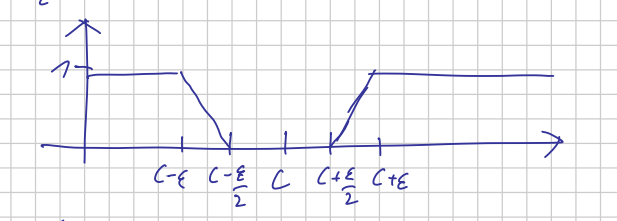
\includegraphics[scale=0.7]{3_4.png}\\
für $\varepsilon>0$.\\
Aus $X_n\xr{d}X$ folgt $P(|X_n-C|>\varepsilon)=\int \1{\brac{|X_m-C|>\varepsilon}}d\underbrace{P(X_n)}_{\mc{L}X_n}\leq\int f_\varepsilon dP(X_n)=E(f_\varepsilon(X_n))\xr[n\toinf]{}E(f_\varepsilon(C))=0$
\item klar, da $\forall f\in\lp{p}(\R)$ gilt $f\circ h\in\cb{}$\QED
Die Umkehrung von Aussage a) ist falsch, ebenso ist es falsch aus $X_n\xr{d}X$ zu folgern, dass $P(X_n\in\mc{A})\ra P(X\in\mc{A})\ \forall\mc{A}\in\mc{B}(\R)$
\end{enumerate}









\subsection{Definition (Quantilfunktion)}
\marginpar{5.Vorlesung, 26.05.2018}
\label{3.5}
Sei $F(x)=P(X\leq x)$ die Verteilungsfunktion einer reellen Zufallsvariable X. Für $a\in(0,1)$ heißt $F^\leftarrow:(0,1)\ra\R\\
u\mapsto F^\leftarrow(u)=\inf\brc{t\in\R:F(t)\geq u}$ \\\underline{inverse Verteilungsfunktion/Quantilfunktion} von F oder X.

\subsection{Lemma (Eigenschaften der Quantilfunktion)}
\label{3.6}
Sei F die Verteilungsfunktion einer Zufallsvariablen X. Dann gilt\begin{enumerate}[label=(\alph*)]
\item $F(F\inv(u))\geq u\ \forall u\in(0,1)$\\
\item Ist $F:\R\ra(0,1)$ bijektiv, so ist $F\inv=F^{-1}$
\item $F\inv$ ist (nicht zwangsweise streng) monoton steigend und linksstetig
\item Für $x\in\R$ und $u\in(0,1)$ gilt $F(x)\geq u \LRa x\geq F\inv(u)$
\item $F(F\inv(u))=u\ \forall u\in F(\R)\cap(0,1)$
\end{enumerate}
\beweis
\begin{enumerate}[label=(\alph*)]
\item F ist rechtsstetig $\Ra\inf$ in der Definition von $F\inv$ wird angenommen. Die Behauptung folgt direkt aus der Definition
\item Folgt sofort aus $F(F^{-1}(u))=u$ und Monotonie
\item Übung
\item $x\geq F\inv(u)\xRightarrow{F\nearrow}F(x)\geq F(F\inv(u))\geq u\\
F(x)\geq u\Ra x\geq\inf\brac{t:F(t)\geq u}=F\inv(u)$
\item \glqq$\geq$\grqq \ folgt aus a)\\
Sei $t_0\in\R$ mit $F(t_0)=u\in(0,1)\\
\Ra F\inv(u)=\inf\brac{t:F(t)\geq u}\leq t_0\\
\xRightarrow{F\nearrow}F(F\inv(u))\leq F(t_0)=u$.\QED
\end{enumerate}

\subsection{Satz (Verteilung durch Uniforme Verteilung berechnen)}
\label{3.7}
Sei $X$ eine reellwertige Zufallsvariable mit Verteilungsfunktion F und\\
$U\sim unif(0,1) ($Gleichverteilung auf $(0,1)=$Lebesguemaß auf $(0,1))$\\
Dann gilt\begin{enumerate}[label=(\alph*)]
\item $X\xlongequal{\mc{D}}F\inv(\mc{U}),$\ d.h.\ \ $\mc{L}(X)=\lambda |_{(0,1)}\circ (F\inv)^{-1}$\\
Für $h\in\mc{L}(P(X))$ gilt $\int hdP(X)=\int\limits_0^1h\circ F\inv d\lambda$
\item Ist F stetig, so gilt\\
$F(X)=\mc{U}, d.h. \mc{L}(F(\lambda))=\lambda|_{(0,1)}$\\
Ist $g\in\lp{1}(\lambda|_{(0,1)})$, so gilt\\
$\int\limits_0^1gd\lambda=\int g\circ F dP(X)$
\end{enumerate}
\beweis
Die Aussagen zu den Integralen folgen unmittelbar aus denen zu den Maßen
\begin{enumerate}[label=(\alph*)]
\item $F(x)=P(\mc{U}\leq F(x))=P(F\inv(\mc{U}\leq x)\ \forall x\in\R$
\item F stetig $\xRightarrow{Zwischenwertsatz}(0,1)\subset F(\R)$\\
Mit \hyperref[3.6]{Lemma 3.6 e} folgt $F(F\inv(u))=u\ \forall u\in(0,1)\\
\mc{L}(F(X))=\mc{L}(X)\circ F^{-1}=\lambda|_{(0,1)}\circ(F\inv)^{-1}\circ F^{-1}\\
=\lambda|_{(0,1)}\circ (\underbrace{F\circ F\inv}_{\text{=Identität}})^{-1}=\lambda|_{(0,1)}$\QED
Sobald man eine gleichverteilte Zufallsvariable realisieren/simulieren kann, kann man also eine beliebig verteilte simulieren.
\end{enumerate}

\subsection{Satz (Helly-Bray)}
\label{3.8}
Seien $\folge{X}{n},\ X:\raum\ra\rbor$ Zufallsvariablen mit Verteilungsfunktionen $F_{X_n}, F_X$. Setze\\
$S(F_X)=\brac{t\in\R:F_X(t)\text{ ist stetig in }t}.$\\
Dann sind äquivalent\begin{enumerate}[label=(\alph*)]
\item $X_n\xr[n\toinf]{d}X$
\item $F_{X_n}(tr)\xr[n\toinf]{}F_X(t)\ \forall t\in S(F_X)$
\item $\exists D\subseteq\R$ dicht so, dass\\
$F_{X_n}(t)\xr[n\toinf]{}F_X(t)\forall t\in D$
\end{enumerate}
\beweis
\begin{list}{•}{}
\item $b)\Ra c)$:\\
 Jede Verteilungsfunktion hat maximal abzählbar viele Sprungstellen $\Ra S(F_X)$ ist dicht in $\R$
\item $c)\Ra b)$:\\
Wähle $x_1,x_2\in D$ mit $x_1\leq x\leq x_2$ und $|F_X(x_{1/2})-F_X(x)|<\varepsilon$\\
$\Ra \lsup F_{X_n}(X)\leq \lim\limits_{n\toinf}F_{X_n}(x_2)=F_X(x_2)\leq F_X(x)+\varepsilon$\\
$\liminf F_{X_n}(9x)\geq \lim\limits_{n\toinf}F_{X_n}(x_1)=F_X(X_1)\geq F_X(x)-\varepsilon$\\
Mit $\varepsilon\searrow0$ folgt die Behauptung.
\item $a)\Ra b)$:\\
Sei $x\in S(F_X)$. Dann gibt es $\fe$ ein $\delta>0$ mit $|x-y|\leq\delta\Ra|F_X(x)-F_X(y)|\leq\varepsilon$\\
Betrachte nun die Funktionen $\mc{L}_\varepsilon$ und $\mc{U}_\varepsilon$\\
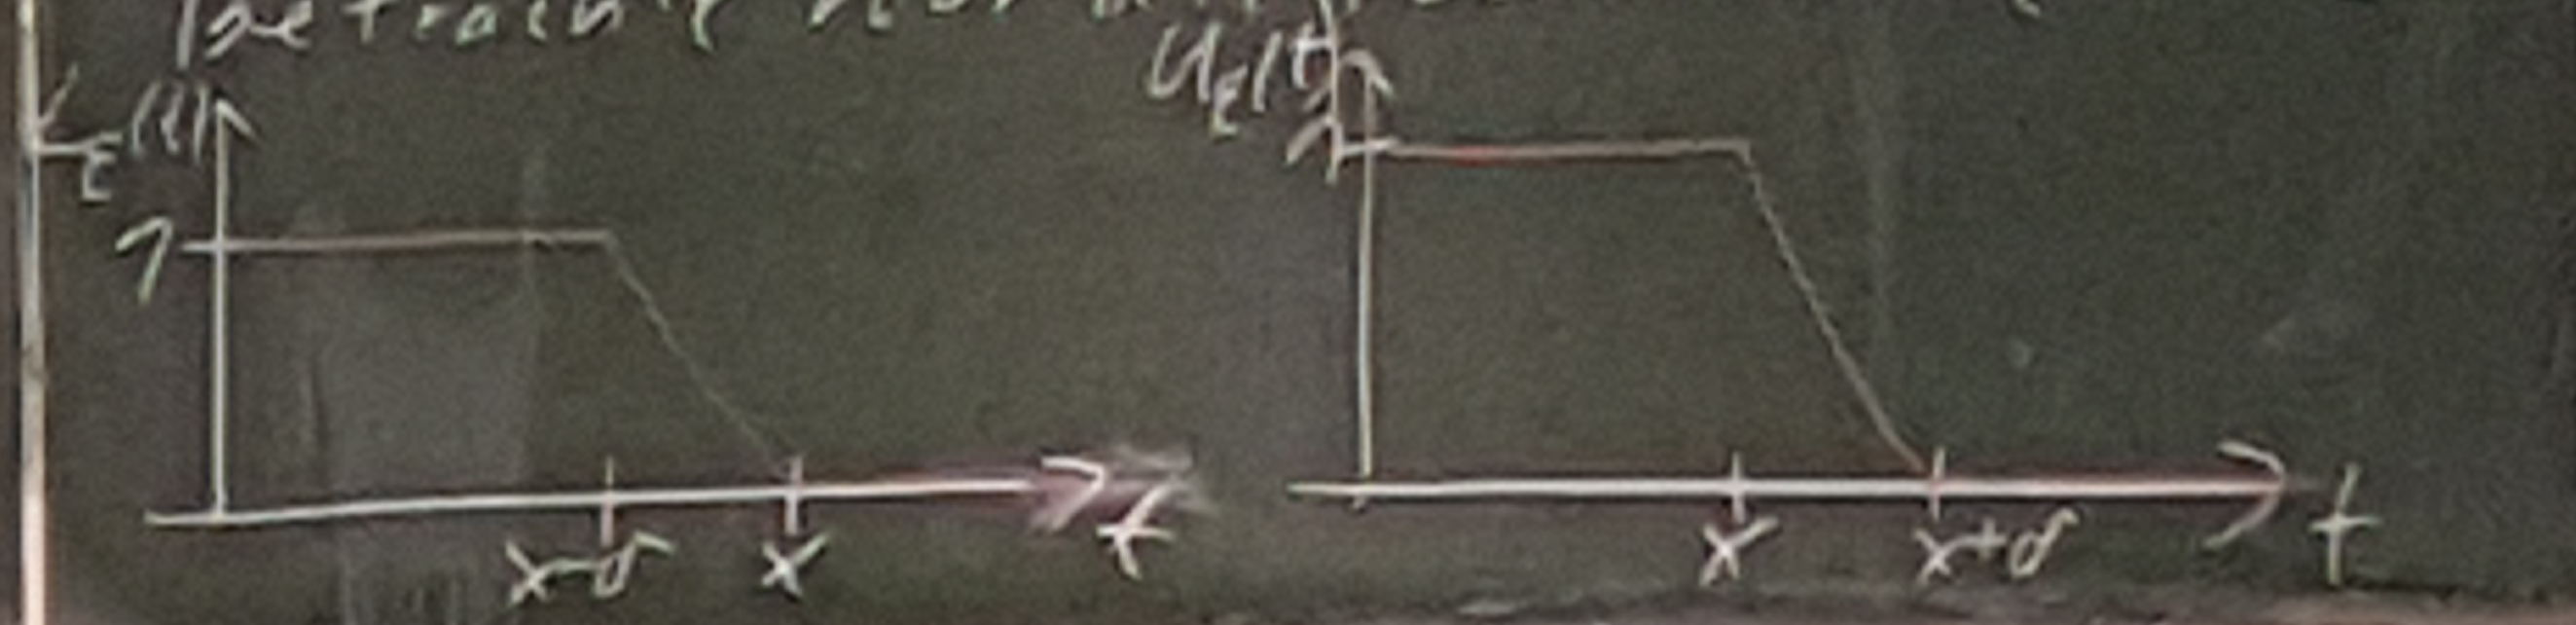
\includegraphics[scale=0.15]{3_8.png}
Dann gilt\\
$\limsup F_{\Xn}(x)=\limsup\int \1{(-\infty,x]}dP(\Xn)\leq\limsup\int \mc{U}_\varepsilon dP(X_n)=\int\mc{U}dP(X)\leq F_X(x+\delta)\leq F_X(x)+\varepsilon\\
\liminf F_{\Xn}(x)\geq\liminf\int \mc{L}_\varepsilon dP(X_n)=\int\mc{L}dP(X)\geq F_X(x-\delta)\leq F_X(x)-\varepsilon$\\
Mit $\varepsilon\searrow0$ folgt $b)$
\item $b)\Ra a)$:\\
Der nächste Satz zeigt: wir können unter $b)$ o.B.d.A. annehmen\\
$X_n\xr[n\toinf]{f.s.}X\Ra X_n\xr{d}X$\QED
\end{list}

\subsection{Satz (Skorohod)}
\label{3.9}
Seien $\folge{X}{n},X$ Zufallsvariablen mit Verteilungsfunktionen $F_{X-n}(t)\ra F_X(t)\forall t\in S(F_X).$ Dann existiert ein Wahrscheinlichkeitsraum $(\widehat\Omega,\widehat\f,\widehat P)$ und Zufallsvariablen $\widehat X_n, \widehat X:(\widehat\Omega,\widehat\f,\widehat P)\ra\rbor$ mit \begin{enumerate}[label=(\alph*)]
\item $\mc{L}(\widehat X_n)=\mc{L}(X_n), \fn, \mc{L}(\widehat X)=\mc{L}(X)$
\item $\widehat X_n\xr{n\toinf}\widehat X\ \widehat P$-f.s.
\end{enumerate}
Wir zeigen zunächst:

\subsection{Lemma}
\label{3.10}
Seien $\folge[\N_0]{F}{n}$ Verteilungsfunktionen mit\\
\[F_n(t)\ra F_0(t) \forall t\in s(F_0)\]\\
Dann gilt\\
\[F_n\inv(t)\ra F_0\inv(t) \forall t\in S(F_0\inv)\cap(0,1)\]






\beweis
\marginpar{6.Vorlesung,  30.04.2018}
Sei $t\in S(F_0\inv),\ 0<t<1$. Zeige zunächst:\\
$\lsup F_n\inv(t)\leq F_0\inv(t)$\begin{flushright}$(*)$\end{flushright}
Sei $t<t'<1$ und $\varepsilon>0$. Dann wähle $x\in S(F_0)$ mit $F_0\inv(t')<x<F_0\inv(t')+\varepsilon$\\
Es gilt $t<t'\leq F_0(F_0\inv(t'))\leq F_0(x)$.\\
Da $F_n(x)\ra F_0(X),$ gibt es ein $n_0$ mit $F_n(x)>t\forall n\geq n_0$.\\
Mit \hyperlink[3.6]{Lemma 3.6 d)} $F_n\inv(t)\leq x\forall n\geq n_0\\
\Ra \lsup F_n\inv(t)\leq x<F_0\inv(t')+\varepsilon$.\\
Mit $t'\searrow t\in S(F_0\inv)$ und $\varepsilon\searrow0$ folgt $(*)$.\\
Analog zeigt man:\\
$\linf F_n\inv(t)\geq F_0\inv(t)$\\
$\Ra$ Behauptung\QED

\textbf{Beweis \hyperref[3.9]{Satz 3.9}}\\
Wähle $(\widehat\Omega,\widehat\f,\widehat P)=((0,1),B((0,1),\lambda|_{(0,1)}$\\
Setze $\widehat X_n=F_{X_n}\inv,\ \widehat X=F_X\inv$. Dann gilt a) mit \hyperref[3.7]{Satz 3.7 a}\\
Zu b): Es Gilt $\widehat P(S(F_X\inv)^c)=0$, da $F_X\inf\nearrow$\\
Somit folgt mit \hyperref[3.10]{Lemma 3.10} aus $F_{X_n}(t)\ra F_X(t)\forall t\in S(F_X)$, dass \\
$F_{X_n}\inv(t)=\widehat X_n(t)\ra F_{X_0}\inv(t)=\widehat X_0(t)$ auf $S(F_X\inv)$ also $\widehat P$-f.s.\QED

\subsection{Proposition}
\label{3.10}
Gilt $X_n\xr{d}X$, dann gilt auch\begin{enumerate}[label=(\alph*)]
\item $\linf E(|X_n|)\geq E(|X|)$
\item $E(X_n)\xr{n\toinf}E(X)$, falls $\folge{X}{n}$ $UI$.
\end{enumerate}
\beweis
\hyperref[3.9]{Satz 3.9} + \hyperref[2.8]{Lemma 2.8/}\hyperref[2.16]{Satz 2.16}\QED


\subsection{Lemma (Slutzky)}
\label{3.12}
Seien $\folge{X}{n}, \folge{Y}{n}, \folge{Z}{n}, X:\raum\ra\rbor[d]$ Zufallsvariablen, $d\in\N$ mit\begin{list}{•}{}
\item $X_n\xr{d}X$
\item $\norm{X_n-Y_n}\xr{p}0$
\item $Z_n\xr{p}c\in\R^d$
\end{list}
Dann gelten:\begin{enumerate}[label=(\alph*)]
\item $Y_n\xr{d}X$
\item $\mat{X_n\\Z_n}\ra \mat{X\\c}$
\item $X_n+Z_n\xr{d}X+c$
\item $X_n^TZ_n\xr{d}X^Tc$
\end{enumerate}
\beweis
\begin{enumerate}[label=(\alph*)]
\item In der Übung wird gezeigt:\\
Es genügt zu zeigen $E(f(Y_n))\ra E(f(x))\forall f\in \cb[]$ mit f gleichmäßig stetig\\
Sei also $f\in C(\R^d,\R\text{, }\norm{f}_{\infty}\leq M$
 und $|f(x)-f(y)|\leq K\norm{x-y}$ für\\
 $M,K>0$. Dann gilt\\
$|E(f(X_n)-f(Y_n))|\leq E(|f(X_n)-f(Y_n)|*(\1{\brac{\norm{X_n-Y_n}\\
\leq\varepsilon}}+\1{\brac{\norm{X_n-Y_n}>\varepsilon}})\\
\leq K\varepsilon+2MP(\norm{X_n-Y_n}\geq\varepsilon)\xr[\varepsilon\searrow0]{n\toinf}0\\
\Ra E(f(Y_n))\xr[n\toinf]{}\lim\limits_{n\toinf}E(f(X_n))=E(f(X))$.
\item Es gilt $\norm{\mat{X_n\\Z_n}-\mat{X_n\\C}}\ra 0$ und $\mat{X_n\\C}\xr{d}\mat{X\\C}$. Nun wende a) an.
\item Folgt aus b) mit dem \hyperref[2.6]{continuous mapping theorem}
\item Folgt aus b) mit dem \hyperref[2.6]{continuous mapping theorem}
\end{enumerate}\QED

\subsection{Beispiel}
\label{3.13}
Seien $\folge{X}{n}\sim N(0,1)$ iid. Dann folgt\\
$T_n=\dfrac{X_0}{\sqrt{\dfrac{1}{n}\sm[n]{i=1}X_i^2}}$ eine $t_n$-Verteilung.\\
Nach dem starken Gesetz der großen Zahlen gilt $\dfrac{1}{n}\sm[n]{i=1}X_i^2\xr[f.s.]{n\toinf}1$\\
Mit Slutzky folgt $T_n\xr{d}\dfrac{X_0}{1}\sim N(0,1)$

\subsection{Definition}
\label{3.14}
\begin{enumerate}[label=(\alph*)]
\item Eine Folge $\folge{P}{n}$ von Wahrscheinlichkeitsmaßen auf $\R$ heißt straff, falls $\forall\varepsilon>0$ ein $k>0$ existiert mit\\
$\sup\limits_{n\in\N}P_n([-K,K]^c)\leq\varepsilon$
\item Eine Folge $\folge{X}{n}$ von Zufallsvariablen heißt straff, falls $(\mc{L}(X_n))_{n\in\N}$ straff ist.
\end{enumerate}

\subsection{Satz (Prohorov)}
\label{3.15}
Jede straffe Folge von Zufallsvariablen besitzt eine in Verteilung konvergente Teilfolge von Zufallsvariablen\\
\beweis
Sei $F_n$ die Verteilungsfunktion von $X_n$ und $\mc{D}=\brac{x_m:m\in\N}$ eine abzählbare dichte Teilmenge von $\R$.\\
Für $m\in\N$ betrachte die Folge $(F_n(x_m))_{n\in\N}$. Nach Bolzano-Weierstraß existiert eine Teilfolge  $(n_{k,1})_{k\in\N}$ so, dass $(F_{n_{k,1}}(x_1)_{k\in\N}$ konvergiert. Wiederum existiert eine Teilfolge $(n_{k,2})_{k\in\N}\subset(n_{k,1})_{k\in\N}$ sodass $(F_{n_{k,2}}(x_2)_{k\in\N}$ konvergiert. Iterativ erhält man Teilfolgen $(n_{k,l})_{k\in\N}$ \ $\fn[l]$ mit $(F_{n_{k,l}}(x_i)_{k\in\N}$ konvergent $\forall i\leq l$.\\
Setze $n_k=n_{k,k}\ \forall k\in\N$.\\
Dann gilt $F_{nk}(x_i)$ konvergiert $\fn[i]$. Definiere nun $G:\mc{D}\ra[0,1]$ durch $G(x_i)=\lim\limits_{n\toinf}F_{n_k}(x_i)$ und setze $G$ auf $\R$ fort durch $F(x):=inf\brac{G(y):y\in\mc{D},y>x}$.\\
Gemäß Konstruktion ist F monoton wachsend und rechtsstetig.\\
F ist sogar eine Verteilungsfunktion, da wegen der Straffheit für jedes $\varepsilon>0$ ein $k\in\N$ existiert mit $F(x)<\varepsilon\forall x<-k$ und $F(x)>1-\varepsilon \forall x>k$ und somit $\lim\limits_{x\ra -\infty}F(x)=1$ gilt.\\
Sei nun $x\in S(F)$. Dann gibt es zu jedem $\varepsilon>0$ $y,z\in\mc{D}$ nut $y<x<z$ und $l_0\in\N$ so, dass \\
$F(x)-\varepsilon\leq G(y)\leq F(x)\leq G(z)\leq F(x)+\varepsilon$ und\\
$F(x)-2\varepsilon\leq F_{n_l}(y)\leq F_{n_l}(x)\leq F_{n_l}(z)\leq F_{n_l}(x)+2\varepsilon \forall l\geq l_0\\
\Ra F(x)-2\varepsilon\leq\linf F_{n_l}(x)\leq \lsup F_{n_l}(x)\leq F(x)+2\varepsilon\\
\xRightarrow{\varepsilon\searrow0}F_{n_l}(x)\xr{l\toinf}F(x)$\\
Mit \hyperref[3.8]{Helly-Bray} folgt die Behauptung.







\pagebreak
\section{Charakteristische Funktionen}
Wie üblich definieren wir für $f:\R^d\ra\C$ messbar das Integral \\
$\int fd\mu=\int Re(f)d\mu+i\int Im(f)d\mu$ und (praktisch) alle Aussagen aus der Integrationstheorie bleiben mit den offensichtlichen Anpassungen gültig.

\subsection{Definition}
\label{4.1}
\begin{enumerate}[label=(\alph*)]
\item Sei $\mu$ ein Wahrscheinlichkeitsmaß auf $\R^d$. Dann heißt \\
$\widehat\mu:\R^d\ra\C, t\mapsto\int e^{i \langle x,t\rangle}\mu(dx)$\\
die \underline{Fouriertransformierte von $\mu$}.
\item Sei $x:\raum\ra\rbor$ eine Zufallsvariable. Dann heißt \\
$\varphi_X(t)=\widehat{P^X}(t)=E(e^{i\langle X,t\rangle})$\\
die charakteristische Funktion von $X$.
\end{enumerate}
\marginpar{7.Vorlesung, 03.05.2018}
Im Folgenden betrachten wir der Einfachheit halber fast immer nur $d=1$. Praktisch alle Aussagen lassen sich unmittelbar auf beliebige Dimensionen Verallgemeinern. Da $|e ^{i\langle x,t\rangle}|\leq 1\forall x,t\in\R^d$ und $\mu(\R^d)=1$ existiert die Fouriertransformierte stets.

\subsection{Satz}
\label{4.2}
Sei $\mu$ ein Wahrscheinlichkeitsmaß auf $\rbor$. Dann gelten:
\begin{enumerate}[label=(\alph*)]
\item $\widehat\mu(0)=1, |\widehat\mu(t)|\leq 1\forall t\in\R^d$
\item $\widehat\mu(\cdot)$ ist gleichmäßig stetig
\item Für $a,b\in\R, X$ reellwertige Zufallsvariable\\
$\varphi_{aX+b}(t)=e^{ibt}\varphi_X(at)$
\item $\varphi_{-X}=\overline{\varphi_X}$
\item \begin{enumerate}
\item Sei $\vartheta$ ein weiteres Wahrscheinlichkeitsmaß auf $\R$:\\
$\widehat{\mu*\vartheta}=\widehat\mu*\widehat\vartheta$
\item Seien $X_1, X_2:\Omega\ra\R$ unabhängige Zufallsvariablen:\\
$\varphi_{X_1+X_2}(t)=\varphi_{X_1}(t)Y_{X_2}(t)$
\end{enumerate}
\item $\widehat{\mu}$ ist positiv semidefinit, d.h. $\forall x_i\in\R, \lambda_i\in\C, n\in\N$ gilt \\
$\sm[n]{j,l=1} \lambda_j\overline{\lambda_l}\widehat{\mu}(x_j-x_l)\geq0$.
\end{enumerate}

\beweis
\begin{enumerate}[label=(\alph*)]
\item Trivial
\item $\sup\limits_{t\in\R}|\varphi_X(t+h)-\varphi_X(t)|\\
=\sup\limits_{t\in\R}|E(e^{itX}(e^{ihx}-1))|\\
\leq \sup\limits_{t\in\R}E(\underbrace{|e^{itx}|}_{=1}|e^{ihx}-1|)\\
=E(|e^{ihx}-1|)\xr[\substack{dom. \\Konv.}]{h\ra0}0$
\item $\varphi_{aX+b}(t)=E(e^{i(aX+b)t})=\underbrace{e^{iaXt}}_{\varphi_X(at)}e^{ibt}$
\item $\overline{\varphi_X(t)}=\overline{E(e^{iXt})}=E(\overline{e^{iXt}})=E(e^{-iXt})=\varphi_{-X}(t)$
\item $\varphi_{X_1+X_2}(t)=E(\underbrace{e^{it(X_1+X_2)}}_{|\cdot|\leq1})\\
=\int_{\R^2}e^{it(X_1+X_2)}d(P^{X_1}\otimes P^{X_2})(X_1, X_2)\\
=\int\limits_\R\int\limits_\R e^{itX_1}e^{itX_2}dP^{X_1}(X_1)dP^{X_2}(X_2)\\
=\int\limits_\R e^{itX_1}dP^{X_1}(X_1)\int\limits_\R e^{itX_2}dP^{X_2}(X_2)\\
=\varphi_{X_1}(t)\varphi_{X_2}(t)$
\item Es gilt\\
$\sm[n]{j,l=1} \lambda_j\overline{\lambda_l}\widehat{\mu}(x_j-x_l)=\int\limits_\R\sm[n]{j,l=1}\lambda_j\overline{\lambda_l}e^{i(x_j-x_l)z}\mu(dz)\\
=\int\limits_\R\sm[n]{j,l=1}\lambda_je^{ix_jz}\overline{\lambda_le^{ix_lz}}\mu(dz)\\
=\int\limits_\R|\sm[n]{j=1}x_je^{ix_jz}|^2\mu(dz)>0$.\QED
\end{enumerate}

\subsection{Bemerkung}
\label{4.3}
\begin{enumerate}[label=(\alph*)]
\item Der Satz von Bochner besagt: Ist $\varphi:\R\ra\C$ positiv semidefinit, $\varphi(0)=1$ und $\varphi$ stetig, dann gibt es ein Wahrscheinlichkeitsmaß $\mu$ mit $\varphi=\widehat\mu$.
\item Gilt $X\xlongequal{d}-X$ (d.h. X ist symmetrisch um Null verteilt), so folgt\\
$Im(E(e^{iuX}))=E(sin(uX))=0$
\end{enumerate}

\subsection{Beispiel}
\label{4.4}
\begin{enumerate}
\item Sei $X\sim$ Bernoulli$(p)$:\\
$\varphi_X(t)=e^{it}P(X=1)+e^0P(X=0)=pe^{it}+(1-p)$
\item Sei $X\sim$ Binomial (n,p)\\
$\varphi_X(t)$\hyperref[4.2]{$\xlongequal{4.2 c}$}$(pe^{it}+(1-p))^n$
\item Sei $X\sim N(\mu,\sigma).$ Dann ist\\
$\varphi_X(t)=exp\brc{i\mu t-\dfrac{1}{2}\sigma^2t^2}$
\end{enumerate}
\beweis
Mit \hyperref[4.2]{Satz 4.2 c)} genügt es, die Aussage für $\mu=0, \sigma^2=1$ zu zeigen. Sei $Y\sim N(0,1)$, dann ist $Y$ symmetrisch um 0 verteilt.
$\varphi_Y(t)=Re\varphi_Y(t)=\dfrac{1}{\sqrt{2\pi}}\int\limits_\R cos(tx)e^{-\dfrac{x^2}{2}}dx\\
\dfrac{d}{dt}\varphi_Y(t)=\dfrac{1}{\sqrt{2\pi}}\int\limits_\R sin(tx)\brc{-x^{-\dfrac{x^2}{2}}}dx\\
\xlongequal{\substack{part.\\int.}}=\dfrac{1}{\sqrt{2\pi}}\brc{sin(tx)e^{-\dfrac{x^2}{2}}|_{-\infty}^\infty-t\int\limits_\R cos(tx)e^{-\dfrac{x^2}{2}}dx}=t\varphi_Y(t)\\
\Ra \dfrac{\dfrac{d}{dt}\varphi_Y(t)}{\varphi_Y(t)}=-t\\
\Ra\dfrac{d}{dt}ln\varphi_Y(t)=-t $(in einer Nullumgebung wo $\varphi_Y(t)>0$)\\
Außerdem gilt $ln\varphi_Y(0)=0\\
\Ra ln\varphi_X(t)=-\dfrac{t^2}{2}\\
\Ra \varphi_X(t)=e^{-\dfrac{1}{2}t^2}$ (in einer Nullumgebung aber damit auf $\R$ da $e^{-\dfrac{1}{2}t^2}>0\forall t\in\R$\QED
Hat $\mu$ Dichte f, so gilt\\
$\widehat\mu(t)=\int e^{itz}\mu(dz)=\int e^{itz}f(z)dz=:\widehat{f}(t)$.
Die Fouriertransformierte des Maßes ist also die Fouriertransformierte (im klassischen analytischen Sinn) der Dichte.

\subsection{Satz (Eindeutigkeitssatz)}
\label{4.5}
Seien $\mu_1,\mu_2$ Wahrscheinlichkeitsmaße auf $\rbor$. Dann gilt \\
$\widehat{\mu_1}=\widehat{\mu_2}\LRa\mu_1=\mu_2$.\\
Für Zufallsvariablen $X,Y$ gilt also\\
$X\xlongequal{d}Y\LRa \varphi_X=\varphi_Y$.

\subsection{Beispiel}
\label{4.6}
Mithilfe der charakteristischen Funktion lassen sich Faltungen gegebenenfalls leicht berechnen.\\
Seien $X_1\sim N(\mu_1,\sigma_1^2), X_2\sim N(\mu_2,\sigma_2^2)$ unabhängig. \\
Dann gilt $X_1+X_2\sim N(\mu_1+\mu_2,\sigma_1^2+\sigma_2^2)$, da \\
$\varphi_{X_1+X_2}(t)=\varphi_{X_1}(t)\varphi_{X_2}(t)=e^{i\mu_1t-\dfrac{1}{2}\sigma_1^2t^2}e^{i\mu_2t-\dfrac{1}{2}\sigma_2^2t^2}\\
=e^{i(\mu_1+\mu_2)t-\dfrac{1}{2}(\sigma_1^2+\sigma_2^2)t^2}$.
Um Siatz 4.5 zu beweisen, zeigen wir zunächst:

\subsection{Lemma}
\label{4.7}
Seien $\mu,\nu$ Wahrscheiunlichkeitsmaße auf $\rbor$. Dann gilt\\
$\int\limits_\R e^{-ixt}\widehat{\mu}(x)d\nu(x)=\int\limits_\R\widehat{\nu}(z-t)d\mu(z).$\\
\beweis
$\int\limits_\R e^{-ixt}\widehat{\mu}(x)d\nu(x)=\int\limits_\R\int\limits_\R e^{-ixt}e^{izx}\mu(dz)\nu(dx)\\
\xlongequal{Fubini}\int\limits_\R\int\limits_\R e^{i(z-t)x}\nu(dx)\mu(dz)=\int\limits_\R\widehat\nu(z-t)\mu(dz)$\\
\\
\textbf{Beweis von Satz 4.5}\\
\glqq $\La$ \grqq \ klar\\
\glqq $\Ra$ \grqq\begin{enumerate}
\item Sei $\nu=N(0,a^{-2})$ für $a>0$ und $\mu$ ein beliebiges Wahrscheinlichkeitsmaß. Mit \hyperref[4.7]{Lemma 4.7} gilt\\
$\int\limits_\R e^{-ixt}\widehat{\mu}(x)d\nu(x)=\dfrac{a}{\sqrt{2\pi}}\int e^{-ixt}\widehat{\mu}(x)e^{-\dfrac{1}{2}x^2a^2}dx\\
=\int\limits_\R e^{-\dfrac{1}{2}a^{-2}(z-t)^2}\mu(dz)\\
\dfrac{1}{2\pi}\int e^{-ixt}\widehat{\mu}(x)e^{-\dfrac{1}{2}a^2x^2}dx = \int\dfrac{1}{\sqrt{2\pi}}e^{-\dfrac{1}{2a^2}(z-t)^2}\mu(dz)\\
=$ Dichte von $N(0,a^2)*\mu$ an der Stelle t.\\
Somit gilt \\
$(*)\widehat{\mu_1}=\widehat{\mu_2}\Ra N(0,a^2)*\mu_1=N(0,a^2)*\mu_2 \forall a>0$
\item Wir zeigen nun:
$(**) a_n\searrow0\Ra N(0,a_n^2)\xr{\omega}\delta_0$\\
Sei $X_n\sim N(0,a_n^2).$ Dann gilt mit \tscheb\\
$P(|X_n|\geq\varepsilon)\leq\dfrac{a_n^2}{\varepsilon^2}\ra0$ für $n\toinf\forall\varepsilon>0$\\
$\Ra X_n\xr{p}0\Ra X_n\xr{d}0$.
\item Seien $Y_1\sim\mu_1, Y_2\sim\mu_2$ und $X_n\sim N(0,a_n^2), n\in\N$, unabhängig. \\
Dann gilt mit \hyperref[3.12]{Slutzky}
$(***) X_n+Y_i\xr[n\toinf]{d}Y_i$ für $i=1,2$\\
$\Ra \underbrace{P^{X_n+Y_1}}_{\xr{d}\mu_1}=P^{X_n}*P^{Y_1}=N(0,a_n^2)*\mu_1=\underbrace{N(0,a_n^2)*\mu_2}_{\xr{d}\mu_2}$\\
$\Ra \mu_1=\mu_2$.\QED
\end{enumerate}

\subsection{Satz (Stetigkeitssatz von Levy)}
\label{4.8}
Seien $\mu_n, \mu$ Wahrscheinlichkeitsmaße auf $\rbor[]$, so gilt:
\begin{enumerate}[label=(\alph*)]
\item $\mu_n\xr[n\toinf]{\omega}\mu\Ra\widehat{\mu}_n(t)\xr[n\toinf]{}\widehat{\mu}(t)\forall t\in\R$.
\item $\widehat{\mu}_n(t)\xr[n\toinf]{}Y(t)$ punktweise mit $Y:\R\ra\C$ stetig in Null $\Ra\exists$ Wahrscheinlichkeitsmaß $\mu$ mit $\widehat{\mu}=Y$ und $\mu_n\xr{\omega}\mu$ für $n\toinf$.
\end{enumerate}





\subsection{Bemerkung}
\label{4.9}
\marginpar{8.Vorlesung, 07.05.2018}
\begin{enumerate}
\item Seien $X_n, X$ Zufallsvariablen, so gilt:\\
$X_n\xr{d}X\LRa\varphi_{X_n}(t)\ra\varphi_X(t)\forall t\in\R$
\item Die Konvergenz in \hyperref[4.8]{Satz 4.8 a)} ist sogar lokal gleichmäßig
\end{enumerate}

\subsection{Lemma}
\label{4.10}
Sei $\mu$ ein Wahrscheinlichkeitsmaß auf $\rbor[]$. Dann gilt:\\
$\mu\brc{\brac{x:|x|\geq\dfrac{1}{\lambda}}}\leq\dfrac{7}{\lambda}\int\limits_0^\lambda1-Re(\widehat{\mu}(t))dt$\\
\beweis
$\lambda^{-1}\int\limits_0^\lambda\underbrace{1}_{\intr 1\mu(dx)}-\underbrace{Re(\widehat{\mu}(t))}_{\intr cos(xt)\mu(dx)}dt=
\lambda^{-1}\int\limits_0^\lambda\intr(1-cos(xt))\mu(dx)dt\\
\xlongequal{Fubini}\intr\lambda^{-1}\int\limits_0^\lambda(1-cos(xt))dt\mu(dx)\\
\geq\int\limits_{\brac{x:|x|\geq\lambda^{-1}}}\lambda^{-1}\brc{t-\dfrac{sin(xt)}{x}}\Bigg|_{t=0}^\lambda\mu(dx)\\
=\int\limits_{\brac{x:|x|\geq\lambda^{-1}}}\brc{1-\dfrac{sin(\lambda x}{\lambda x}}\mu(dx)\\
\geq \int\limits_{\brac{x:|x|\geq\lambda^{-1}}}(1-sin(1))\mu(dx)\geq\dfrac{1}{7}\mu\brac{x:|x|\geq\lambda^{-1}}$\\
Denn $\dfrac{sin(t)}{t}\leq sin(1)\leq\dfrac{6}{7}\forall t\geq 1$\QED

\textbf{Beweis von \hyperref[4.8]{Satz 4.8}}
\begin{enumerate}[label=(\alph*)]
\item Offensichtlich, da $sin(\cdot t), cos(\cdot t)\in\cb[]\forall t$
\item Wegen $\varphi(0)=1$ und der Stetigkeit in 0 gilt:\\
$\fe\exists\lambda>0$ mit\\
$1-Re\varphi(t)\leq\dfrac{\varepsilon}{7}\forall t\in[-\lambda,\lambda]$ (da $Im\varphi(t)\xr[t\ra0]{}0$) \\
und $Re\varphi(t)\xr[t\ra0]{}1$.
Mit \hyperref[4.10]{Lemma 4.10} folgt\\
$\lsup \mu_n(\brac{x:|x|\geq\lambda^{-1}})\leq\lsup\dfrac{7}{\lambda}\int\limits_0^\lambda\underbrace{(1-Re\widehat{\mu}_n(t))}_{\substack{\ra 1-Re\varphi(t)\\|\cdot|\leq 2}}dt\\
=\dfrac{7}{\lambda}\int\limits_0^\lambda\underbrace{(1-Re(\varphi(t))}_{\leq\dfrac{\varepsilon}{7}}dt\leq\varepsilon$\\
Somit gibt es $\fe$ ein $n_0\in\N$ so, dass $\mu_n((-\lambda,\lambda)^c)\leq2\varepsilon$\\
Es folgt, dass $\folge{\mu}{n}$ straff ist.\\
Nach dem \hyperref[3.15]{Satz von Prohorov} gibt es eine Teilfolge $\folge{n}{l}$ und ein Wahrscheinlichkeitsmaß $\mu$ mit $\mu_{n_l}\xr{\omega}\mu, l\toinf$\\
$\xRightarrow{a)}\widehat{\mu}_{n_l}\ra\widehat{\mu}$ punktweise $\Ra\widehat{\mu}=\varphi$\\
Angenommen $\mu_n\not\xrightarrow{\omega}\mu$. Dann $\exists f\in\cb[]$ und eine Teilfolge $\folge{n}{k}$ mit\\
$\left|\int fd\mu_{n_k}-\int fd\mu\right|>\varepsilon\forall k\in\N$.\\
Nun gibt es aber eine weitere Teilfolge $\brc{n_{k_l}}_{l\in\N}$ mit $\mu_{n_{k_l}}\xr{\omega}\mu\ \wid$\QED
\end{enumerate}

\subsection{Korollar}
\label{4.11}
Seien $X_n,Y_n:\raum\ra\rbor[]$ (für gleichen Index) unabhängige Zufallsvariablen  für $n\in\N_0$ mit $X_n\xr{d}X_0,Y_n\xr{d}Y_0$.\\
Dann gilt $X_n+Y_n\xr{d}X_0+Y_0$.\\
\beweis
$\varphi_{X_n+Y_n}=\varphi_{X_n}\varphi_{Y_n}\xr{pktweise}\varphi_{X_0}\varphi_{Y_0}=\varphi_{X_0+Y_0}$\QED

\subsection{Satz (Fourierinversion)}
\label{4.12}
Sei $\mu$ ein Wahrscheinlichkeitsmaß auf $\rbor[]$ mit $\intr|\widehat{\mu}(x)|dx<\infty$\\
Dann ist $\mu$ absolutstetig (bzgl. des Lebesguemaßes) mit stetiger und beschränkter Dichte\\
$f(t)=\intr\dfrac{1}{2\pi}e^{-ixt}\widehat{\mu}(x)e^{-\dfrac{a^2x^2}{2}}dx$\\
\beweis
Aus dem Beweis von \hyperref[4.5]{Satz 4.5} wissen wir, dass $N(0,a^2)*\mu$ die Dichte\\
$f_a(t)=\dfrac{1}{2\pi}\intr e^{-ixt}\widehat{\mu}(x)e^{-\dfrac{a^2x^2}{2}}dx$ hat (für $a>0$)\\
$\Ra |f(t)|\vee|f_a(t)|\leq\dfrac{1}{2\pi}\intr|\widehat{\mu}(x)|dx<\infty\forall t\in\R$\\
Mittels dominierter Konvergenz folgt\\
$f_a(t)\xr{a\ra0}f(t)$\\
In allen Stetigkeitsstellen von $\mu$ gilt \\
$\int\limits_{(-\infty,x]}f_a(x)dx=N(0,a^2)*\mu((-\infty,x])\xr[a\searrow0]{}\mu((-\infty,x])   (*)$\\
und andererseits gilt \\
$\int\limits_{(y,x]}f_a(x)dx\xr[\substack{dom.\\konv.}]{a\ra0}\int\limits_{(y,x]}f(x)dx\xlongequal{(*)}\mu((y,x])$\\
(falls $y,x$ stetigkeitsstellen von $\mu$)\\
$\xRightarrow{Monotonie}\int\limits_{(-\infty,x]}f(x)ds=\mu((-\infty,x])$ $(\forall$ Stetigkeitsstellen $x$ von $\mu$)\\
$\Ra f$ ist Dichte von $\mu$.\\
f ist beschränkt und stetig folgt aus $\widehat{\mu}\in\lp{1}$ und dominierter Konvergenz\QED

\subsection{Proposition (Cramer-Wold-Device)}
\label{4.13}
Seien $\folge{X}{n}, X:\raum\ra\rbor$ Zufallsvariablen. Dann sind äquivalent:\begin{enumerate}[label=(\alph*)]
\item $X_n\xr{d}X, n\toinf$
\item $\langle \lambda,X_n\rangle\xr[n\toinf]{d}\langle\lambda,X\rangle\forall\lambda\in\R^d$
\end{enumerate}
\beweis
\begin{list}{•}{}
\item $a)\Ra b)$\\
folgt aus dem \hyperref[2.6]{continuous mapping theorem}, da $x\mapsto\langle \lambda,x\rangle$ stetig ist für $\lambda\in\R^d$
\item $b)\Ra a)$\\
Für alle $t\in\R^d$ gilt\\
$\varphi_{X_n}(t)=E\brc{e^{i\langle t,X_n\rangle}}\xr{b}E\brc{e^{i\langle t,X\rangle}}=\varphi_X(t)\\
\Ra \varphi_{X_n}\ra\varphi_X$ punktweise $\xRightarrow[satz v. Levy]{Stetigkeits-} X_n\xr{d}X$\QED
\end{list}
\subsection{Satz}
\label{4.14}
Sei $X\in\lp{n}$ für ein $n\in\N$. Dann ist $\varphi_x$ n-fach stetig differenzierbar mit \\
$\varphi_x(t)^{(r)}=i^r\intr e^{ixt}x^rdP^X(x)$\\
und es gilt\\
$E(X^r)=i^{-r}\varphi_X^{(r)}(0)$\\
für $r=1,...,n$\\
\beweis
n=1: \\
Sei $X\in\lp{1}\\
\dfrac{\varphi_X(t+h)-\varphi_X(t)}{h}=E\Bigg(\underbrace{e^{itX}}_{|\cdot|\leq 1}\Bigg(\underbrace{\dfrac{e^{ihX}-1}{h}}_{\substack{\xr{h\ra0}iX\\|\cdot|\leq|X|}}\Bigg)\Bigg)\\
\xr[n\ra0]{dom.Konv.}E\big(e^{itX}iX\big)=i^1\intr e^{ixt}xdP^X(x)\\
\Ra$ differenzierbar mit stetiger Ableitung\\
$\dfrac{d}{dt}\varphi_X(t)\Bigg|_{t=0}=i^1\int xdP^X(x)=iE(X)$\\
$n=2,3,...$ Analog per Induktion\QED

Eng verbunden mit der charakteristischen Funktion ist die momenterzeugende Funktion / Laplacetransformierte eines Maßes / einer Zufallsvariable:\\
$\R\ra\R, t\mapsto E(e^{tX})=:M_X(t)$ \ \ \glqq $=\varphi_X(it)$\grqq\\
Diese muss für kein t (außer 0) existieren! Für positive Zufallsvariablen existiert sie für $t\in(-\infty,0]$.\\
Existiert die Laplacetransformierte in einer Nullumgebung, so sind alle Momente endlich $(X\in\lp(p)\forall p>0)$.





\pagebreak
\section{Zentrale Grenzwertsätze}
\marginpar{9. Vorlesung, 15.05.2018}
Sei $\folge{X}{i}$ eine iid (independent identically distributed) Folge von Zufallsvariablen mit $X_1\in\lp{2}$.\\
Setze  $\mu=E(X_1), \sigma^2=Var(X_1)$.\\
Wir nehmen von nun an an $\sigma^2>0$.\\
Für $n\in\N$ definieren wir\\
$S_n=\dfrac{\sm[n]{i=1}X_i-n\mu}{\sqrt{n}\sigma}$.\\
Dann gilt $E(S_n)=0, Var(S_n)=1$.

\subsection{Satz (ZGWS klassisch)}
\label{5.1}
Unter obigen Voraussetzuzngen gilt\\
$S_n\xr[n\toinf]{d}N(0,1)$\\
\beweis
Setze $Y_i=\dfrac{1}{\sigma}(X_i-\mu)$. Dann gilt $S_n=\dfrac{1}{\sqrt{n}}\sm[n]{i=1}Y_i$ und $Y_i\in\lp{2}\Ra S_n\in\lp{2}$.\\
Es bezeichne $\nu$ die Verteilung von $Y_1$.\\
Dann gilt mit \hyperref[4.14]{Satz 4.14} und Taylor\\
$\varphi_{Y_1}(x)=\widehat{\nu}(x)=\widehat{\nu}(0)+\widehat{\nu}(0)'x+\dfrac{1}{2}\widehat{\nu}''(0)x^2+o(x^2)\\
=1+\dfrac{1}{2}i^{-2}E(Y_1^2)x^2+o(x^2)=1-\dfrac{1}{2}x^2+o(x^2)\\
\varphi_ {S_n}(x)=\widehat{\nu}\brc{\dfrac{x}{\sqrt{n}}}^n=\brc{1-\dfrac{x^2}{2n}+o\brc{\dfrac{x^2}{n}}}^n\\
=\brc{1+\dfrac{-\dfrac{1}{2}x^2+no\brc{\dfrac{x^2}{n}}}{n}}^n\xr{n\toinf}e^{-\dfrac{1}{2}x^2}=\widehat{N(0,1)}(x)$\QED 

Mit mehr Aufwand und Voraussetzungen kann man die Konvergenzgeschwindigkeit (uniform für die  Verteilungsfunktionen) bestimmen:

\subsection{Satz (Berry-Esséen)}
\label{5.2}
Unter den Voraussetzungen von \hyperref[5.1]{Satz 5.1} und $X_1\in\lp{3}$ gilt\\
$\sup\limits_{t\in\R}|P(S_n\leq t)-\Phi(t)|\leq c\dfrac{E(|X_1|^3)}{\sqrt{n}\sigma}\forall c\geq c^*$ mit $0,4097\leq c*\leq 0,4748$ wobei $\Phi$ die Verteilungsfunktion der Standardnormalverteilung bezeichnet\\
Mit dem starken Gesetz der großen Zahlen und \hyperref[3.12]{Slutzky} folgt sofort:

\subsection{Korollar}
\label{5.3}
Unter den Voraussetzungen von \hyperref[5.1]{Satz 5.1} gilt\\
$\dfrac{\sm[n]{n=1}(X_i-\mu)}{\sqrt{n}\widehat{\sigma}_n}\xr{d}N(0,1)\\ $
mit $\widehat{\sigma}_n^2=\dfrac{1}{n-1}\sm[n]{i=1}\brc{X_i-\dfrac{1}{n}\sm[n]{i=1}X_i}^2$\\
Wir wenden uns nun der Verallgemeinerung des Zentralen Grenzwertsatzes auf Dreiecksschemata von Zufallsvariablen zu. Gegeben seien Zufallsvariablen $X_{nl}:\raum\ra\rbor[]$ mit $\nn ,l\in\brac{1,2,...,n}$, die Zeilenweise unabhängig sind, d.H. $S_{n1},S_{n2},...,S_{nn}$ sind jeweils unabhängig.

\subsection{Satz (Lindeberg-Feller)}
\label{5.4}
Sei $\brc{X_{nl}}_{l\in\brac{1,...,n}},\nn$ ein Dreiecksschema zeilenweise unabhängiger Zufallsvariablen in $\lp{2}$ mit folgenden Eigenschaften:\begin{enumerate}[label=(\alph*)]
\item $ \sm[n]{l=1}E(X_{nl})=0\quad \forall\nn $
\item $ \sm[n]{l=1}Var(X_{nl})\xr{n\toinf}\sigma^2\in(0,\infty)$
\item (Lindeberg-Bedingung):\\
$L_n(\varepsilon):=\sm[n]{l=1}E\brc{X_{nl}^2\1{\brac{|X_{nl}|>\varepsilon}}}\xr{n\toinf}0\quad \fe $
\end{enumerate}
Dann gilt \\
$\sm[n]{i=1}X_{nl}\xr{d}N(0,\sigma^2)$\\
\beweis
Technisch aufwendige Verallgemeinerung des Beweises von \hyperref[5.1]{Satz 5.1}\QED

\subsection{Lemma}
\label{5.5}
Erfüllt ein Dreiecksschema von Zufallsvariablen die Lindeberg-Bedingung, so gilt:\begin{enumerate}[label=(\alph*)]
\item Das Dreiecksschema ist (uniform) asymptotisch vernachlässigbar, d.h.\\
$\max\limits_{l\in\brac{1,...,n}}P(|X_{nl}|>\varepsilon)\xr{n\toinf}0\quad \fe$
\item Es erfüllt die Fellerbedingung, d.h.\\
$\max\limits_{l\in\brac{1,...,n}}Var(X_{nl})\xr{n\toinf}0$	
\end{enumerate}
\beweis
\begin{enumerate}[label=(\alph*)]
\item Folgt aus b) und \tscheb
\item Für $\varepsilon>0$ gilt\\
$Var(X_{nl})\leq E(X_{nl}^2)=E(X_{nl}\1{\brac{|X_{nl]\leq\varepsilon}}})+E(X_{nl}\1{\brac{|X_{nl]>\varepsilon}}})\\
\leq \varepsilon^2+L_n(\varepsilon)\xr[\varepsilon\searrow0]{n\toinf}0.$\QED
\end{enumerate}

\subsection{Lemma}
\label{5.6}
Sei $\folge{X}{i}$ eine Folge von iid Zufallsvariablen in $\lp{2}$ mit $Var(X_1)>0$. Dann erfüllt das Dreiecksschema\\
\[X_{nl}=\dfrac{X_l-E(X_1)}{\sqrt{n}}\]
die Voraussetzungen von \hyperref[5.4]{Satz 5.4.}\\
\beweis
\begin{enumerate}[label=(\alph*)]
\item Zeilenweise unabhängigkeit ist Trivial
\item $\sm[n]{l=1}Var(X_{nl})=\dfrac{1}{n}\sm[n]{l=1}Var(X_l)=Var(X_1)$
\item o.B.d.A sei $E(X_1)=0$. Für $\varepsilon>0$ gilt:\\
$L_n(\varepsilon)=\dfrac{1}{n}\sm[n]{l=1}E\brc{X_l^2\1{\brac{|X_l|>\varepsilon\sqrt{n}}}}=E\brc{\underbrace{X_1^2\1{\brac{|X_1|>\varepsilon\sqrt{n}}}}_{\substack{\xr{n\toinf}0 pktweise\\ \leq X_1^2}}}\xr[n\toinf]{dom. Konv}0$\QED
\end{enumerate}


\subsection{Lemma (Lyapunov-Bedingung)}
\label{5.7}
Sei $X_{nl}$ ein Dreiecksschema von Zufallsvariablen. Existiert ein $\delta>0$ mit $X_{nl}\in\lp{2+\delta}\forall n,l$ und gilt\\
$\sm[n]{l=1}E\brc{|X_{nl}^{2+\delta}}\xr{n\toinf}0$, dann erfüllt das Dreiecksschema die \hyperref[5.4]{Lindebergbedingung}.\\
\beweis
Sei $\varepsilon>0$.\\
$L_n(\varepsilon)=\sm[n]{l=1}E(X_{nl}^2\underbrace{\varepsilon^\delta}_{<|X_{nl}|^\delta}\varepsilon^{-\delta}\1{\brac{|X_{n1}|>\varepsilon}}\leq\varepsilon^{-\delta}\sm[n]{l=1}E\brc{|X_{nl}|^{2+\delta}}\xr{n\toinf}0$

\subsection{Bemerkung}
\label{5.8}
\begin{enumerate}[label=(\alph*)]
\item Interpretiert man $N(0,0)$ als $\delta_0$ so gilt \hyperref[5.4]{Satz 5.4} auch, falls $\delta^2=0$.\\
\beweis
Dann gilt $Var\brc{\sm[n]{l=1}X_{nl}}\ra 0$ und mit \tscheb folgt $\sm[n]{l=1}X_{nl}\xr{p}0$\QED
\item Es gibt Varianten des ZGWS,die keine Unabhängigkeit fordern, dafür aber geeignete asymptotische Unabhängigkeit (und mehr Momente).
\item Es ist auch möglich, ähnliche Resultate für Zufallsvariablen ohne zweite Momente zu zeigen. Die Grenzverteilungen sind dann stabile Verteilungen.
\end{enumerate}





\subsection{Beispiel (Rekorde)}
\marginpar{10.Vorlesung, 17.05.2018} 
\label{5.9}
Sei $\folge{X}{i}$ eine iid Folge von Zufallsvariablen mit $\mc{L}(X_1)$ stetig.\\
\[A_n:=\brac{\max\limits_{1\leq l\leq n-1}X_l<X_n}\quad \widehat{=}\text{neuer Rekord zur Zeit n})(A_1=\Omega)\]\\
Dann gilt für $R_n=\sm[n]{i=1}1_(A_i)$\[
T_n=\dfrac{R_n-ln(n)}{\sqrt{ln(n)}}\xr{d}N(0,1)
\]
\beweis
Aus der Stetigkeit von $X_i$ und $X_i$ iid folgt $P(A_n)=\dfrac{1}{n}$ (unter den ersten n Zufallsvariablen wird das Maximum an den Stellen $1,...,n$ mit der gleichen Wahrscheinlichkeit angenommen)\\
$\Ra 1_(A_n)\sim$ Bernoulli$\brc{\dfrac{1}{n}}$\\
Für $i<j$ gilt $P(A_i\cap A_j)=P(A_i|A_j)P(A_j)=\dfrac{1}{ij}$\\
Induktiv folgt $\brc{1_{A_n}}_{n\in\N}$ sind unabhängig.\[
E\brc{1_{A_n}}=\dfrac{1}{n},\quad Var\brc{1_{A_n}}=\dfrac{1}{n}\brc{1-\dfrac{1}{n}}\\
\sigma_n^2:=\sm[n]{l=1}Var\brc{1_{A_l}}=\sm[n]{l=1}\dfrac{1}{l}\brc{1-\dfrac{1}{l}}\xr{n\toinf}\infty
\]
Setze $X_{nl}=\dfrac{1_{A_l}-\dfrac{1}{l}}{\sigma_n}$.\\
Dann gilt $E(X_{nl})=0,\quad \sm[n]{i=1}Var\brc{X_{nl}}=1$ \\
und wegen $|X_{nl}|\leq\dfrac{2}{\delta_n}\xr{n\toinf}0$ gilt Lindeberg\\
$\Ra\sm[n]{l=1}X_{nl}\xr{d}N(0,1)$\\
Es gilt:\[
T_n=\dfrac{\sm[n]{l=1}\brc{1_{A_l}-\dfrac{1}{l}}}{\sigma_n}\cdot\dfrac{\sigma_n}{\sqrt{log(n)}}+\dfrac{\sm[n]{l=1}\dfrac{1}{l}-log(n)}{\sqrt{log(n)}}\]
$\bullet\qquad\dfrac{\sm[n]{l=1}\dfrac{1}{l}-log(n)}{\sqrt{log(n)}}\ra 0\text{, da gilt }log(n)=\int\limits_1^n\dfrac{1}{n}dx\leq\sm[n]{l=1}\dfrac{1}{l}\leq log(n)+1\\
\bullet\qquad\dfrac{\sigma_n^2}{log(n)}\ra 1$, denn\[
\sigma_n^2=\sm[n]{l=1}\dfrac{1}{l}-\underbrace{\sm[n]{l=1}\dfrac{1}{l^2}}_{\xr{n\toinf}c\in(0,\infty)}
\]\QED

\subsection{Satz (Lindeberg-Feller multivariat)}
\label{5.10}
Sei $X_{nl}:\raum\rbor$ ein Dreiecksschema zeilenweise unabhängiger Zufallsvektoren mit $X_{nl}\in\lp{2}\quad\forall n,l$. Setze $\Sigma_{nl}=Cov(X_{nl})$ \ ($d\times d$ symmetrische strikt positiv definite Matrix). Wenn\begin{enumerate}[label=(\alph*)]
\item $\sm[n]{l=1}E(X_{nl}=0\in\R^d$
\item $\sm[n]{l=1}\Sigma_{nl}\xr{n\toinf}\Sigma $($d\times d$ symmetrische strikt positiv definite Matrix)
\item $L_n(\varepsilon):=\sm[n]{l=1}E\brc{\norm{X{nl}}^2\1{\norm{X_{nl}}>\varepsilon}}\xr{n\toinf}0\quad\forall\varepsilon>0$
\end{enumerate}
dann gilt \[\sm[n]{l=1}X_{nl}\xr{d}N(0,\Sigma)\]
\beweis
Sei $X\in\R^d\backslash\brac{0}$ (beachte $\langle 0,\sm[n]{l=1}X_{nl}\rangle\xr{d}0$ ist klar)\\
Und setze $Y_{nl}=\langle X, X_{nl}\rangle$. Dann gilt\begin{list}{•}{}
\item $\sm[n]{l=1}E(Y_{nl})=\langle X,E\brc{\sm[n]{l=1}X_{nl}}\rangle=0$
\item  $\sm[n]{l=1}Var(Y_{nl})=X^T\brc{\sm[n]{l=1}Cov(X_{nl})}X\ra X^T\Sigma X\in(0,\infty)$
\item $\sm[n]{l=1}E\brc{Y_{nl}^2\2{>_{nl}>\varepsilon}}\overset{CSU}{\le}\sm[n]{l=1}E\brc{\norm{X}^2\norm{X_{nl}}^2\2{|X^TX_{nl}|>\varepsilon}}\\
\overset{CSU}{\le}\norm{X}^2\sm[n]{l=1}E\bigg(\norm{X_{nl}}^2\underbrace{\2{\norm{X}\norm{X_{nl}}>\varepsilon}}_{=\2{\norm{X_{nl}>\dfrac{\varepsilon}{\norm{X}}}}}\bigg)\xr{n\toinf}0$
\end{list}
Somit erfüllt $Y_{nl}$ die Voraussetzungen des  \hyperref[5.4]{eindimensionalen Lindeberg-Feller-Satzes.}\\
Sei $Y\sim N(0,\Sigma),$ dann gilt\\
$\underbrace{\sm{n]{l=1}Y_{[nl}}}_{=X^T\sm[n]{l=1}X_{nl}}\xr{d}X^TY\sim N(0,X^T\Sigma X)$
Mit \hyperref[4.13]{Cramer-Wold-Device} folgt die Behauptung.\QED
 
\subsection{Bemerkung}
\label{5.11}
Lässt man auch degenerierte Normalverteilungen zu (definiert über die charakteristische Funktion $z\mapsto e^{i\langle\mu,z\rangle-\dfrac{1}{2}\langle z,\Sigma z\rangle}$) so genügt es wegen \hyperref[5.8]{Bemerkung 5.8 a)} $\Sigma$ als positiv semidefinit vorauszusetzen.

\subsection{Korollar}
\label{5.12}
Seien $\folge{X}{i}$ iid Zufallsvariablen mit $E(X_1)=\mu$ und $Cov(X_1)=\Sigma\in M_d(\R)$ symmetrisch strikt positiv definit.\\
Dann gilt:\\
$\dfrac{1}{\sqrt{n}}\sm[n]{i=1}{X_i-\mu}\xr{d}Y\sim N_d(0,\Sigma).$\\
Eine weitere wichtige Aussage über das Wachstumsverhalten von iid Partialsummen üver iid Zufallsvariablen gibt der folgende Satz

\subsection{Satz (Gesetz vom iterierten Logarithmus)}
\label{5.13}
Sei $\folge{X}{n}$ eine iid Folge von Zufallsvariablen mit $E(X_1)=0$ und $Var(X_1)=1$.\\
Dann gilt
\[\lsup\dfrac{\sm[n]{i=1}X_i}{\sqrt{2nlog(log(n))}}=1\quad P-f.s.\]
\[\linf\dfrac{\sm[n]{i=1}X_i}{\sqrt{2nlog(log(n))}}=-1\quad P-f.s.\]







\section{Bedingte Erwartungswerte}
\marginpar{11.Vorlesung, 24.05.2018}
Erinnerung an Elementare Wahrscheinlichkeitsrechnung und Statistik:\\
Seien $X:\Omega\ra\R^n,\ Y_\Omega\ra\R^m$ Zufallsvariablen mit gemeinsamer Wahrscheinlichkeitsdichte $f:\R^n\times\R^m\ra\R^+$.\\
Dann ist die bedingte Dichte\\
$f_{X|Y}(x,y)=\dfrac{f(x,y)}{\int\limits_{\R^d}f(z,y)dz}$\\
(eine messbare Funktion in $(x,y)$)\\
und die bedingte Erwartung von $X$ gegeben $Y=y$\\
$E(X|Y=y)=\int\limits_{\R^m}xf_{X|Y}(x,y)dx$\\
eine messbare Funktion von $y$.\\
Entsprechend ist die bedingte Erwartung \\
$E(X|Y)=\int\limits_{\R^m}xf_{X|Y}(x,Y)dx$\\
eine Zufallsvariable (messbare Funktion in $\omega$).\\
$E(X|Y)$ ist offenbar sogar $\sigma(Y)-\mc{B}(\R^n)$-messbar, also eine Zufallsvariable auf $(\Omega,\sigma(Y),P|_{\sigma(Y)})$.\\
Sei $h:\R^m\ra\R$ messbar und beschränkt, $X\in\lp{1}(P)$, dann gilt\\
$E(h(Y)E(X|Y))=\int\limits_{\R^m}h(y)\int\limits_{\R^n}x\dfrac{f(x,y)}{f_Y(y)}dxf_Y(y)dy\\
=\int\limits_{\R^m}\int\limits_{\R^n}h(y)xf(x,y)dxdy=E(h(Y)|X)$

\subsection{Definition und Satz}
\label{6.1}
Sei $X\in\lp{1}(P)$ oder $X\geq0$ und $\g\subseteq\f\quad\sigma-$Algebra.\begin{enumerate}[label=(\alph*)]
\item Dann existiert $Z:\Omega\ra\overline{\R}$ mit \begin{enumerate}[label=(\roman*)]
\item $Z$ ist $\g$-Messbar
\item $E(X1_A)=E(Z1_A)\quad\forall A\in\g$
\end{enumerate}
Man nennt Z die bedingte Erwartung von X gegeben $\g$, i.Z. $Z=E(X|\g)$.
\item $Z$ ist durch 1) und 2) f.s. eindeutig bestimmt.
\end{enumerate}
Seien $\mu,\nu$ zwei Maße auf $(\Omega,F)$.\\
$\mu$ heißt absolutstetig bezüglich $\nu$, (i.Z. $\mu\ll\nu)$, wemm $\nu(A)=0\Ra\mu(A)=0$\\
$\mu$ und $\nu$ heißen äquivalent, wenn $\mu\ll\nu$ und $\nu\ll\mu$

\textbf{Satz von Radon-Nikodym}\\
\label{Radon}
Wenn $\mu\ll\nu$, dann gibt es $Z:\Omega\ra\R^+,\ Z\geq0$ und messbar mit $\int1_Bd\mu=\int1_BZd\nu\quad\forall B\in\f$\\
\grqq$\underbrace{\dfrac{d\mu}{d\nu}}_{\text{Radon-Nikodym-Ableitung}}$\grqq$=Z$
\textbf{Beweis von Satz 6.1}
\begin{enumerate}[label=(\alph*)]
\item \begin{enumerate}[label=(\roman*)]
\item Sei $X\gg0\\
Q:\g\ra\R^+,\ B\mapsto\int\limits_BXdP=E(1_BX)$\\
ein Maß auf $(\Omega,\g)$ mit $Q\ll P|_{\g}\\ $
Nach Radon-Nikodym existiert eine Dichte $Z$ von $Q$ bzgl. $P|_{\g} \g$ d.h. $Z\geq 0$, $\g$-messbar mit \\
$Q(B)=E_P(!_BX)=\int 1_BZdP|_{\g}=E_P(1_BZ)$
\item Sei $X\in\lp{1}(P)$. Zerlege $X=X^+-X^-$. Mit a) existieren $Z^+,Z^-\ \g$-messbar so, dass\\
$E(X^{+/-})=E(Z^{+/-}1_B)\quad\forall B\in\g$\\
Die linearität der Erwartungswerte liefert die Behauptung.
\end{enumerate}
\item Seien $Z_1,Z_2$ Zufallsvariablen die i), ii) erfüllen. Dann gilt\\
$B:=\brac{Z_1>Z_2}\in\g$\\
$E(1_B(\underbrace{Z_1-Z_2}_{>0\text{ auf B}}))\xlongequal{ii)}E(1_B(X-X))=0\\
\Ra P(B)=0$\\
Analog zeigt man $P(\brac{Z_2>Z_1})=0\Ra P(Z_1=Z_2)=1$\QED
\end{enumerate}

\subsection{Satz}
\label{6.2}
Seien $X,Y:\raum\ra\rbor[]$ Zufallsvariablen mit $X,Y\in\lp{1}$ oder $X,Y\geq 0$ und $\g\subseteq\mc{H}\subseteq\f\ \sigma$-Algebren. Dann gelten:\begin{enumerate}[label=(\alph*)]
\item $E(\alpha X+\beta Y|\g)=\alpha E(X|\g)+\beta E(Y|\g)\quad\forall\alpha,\beta\geq0$\\
(bzw. $\forall\alpha,\beta\in\R,$ falls $X,Y\in\lp{1}$)
\item $E(E(X|\g))=E(X)$ und $E(E(X|\g)|\g)=E(X|\g)$
\item $E(E(X|\mc{H})|\g)=E(X|\g)$\ \ (tower priority)
\item $X=Y$ f.s. $\Ra E(X|\g)=E(Y|\g)$ f.s. und\\
 $X\leq Y$ f.s. $\Ra E(X|\g)\leq E(Y|\g)$ f.s.
\item Ist $Y\ \g$-messbar und $XY\in\lp{1}$, dann gilt \\
$E(XY|\g)=YE(X|\g)$ und $E(Y|\g)=Y=E(Y|\underbrace{Y}_{\sigma(Y)})$
\item Sind $\sigma(X)$ und $\g$ unabhängig, dann gilt \\
$E(X|\g)=E(X)$. Insbesondere $E(X)=E(X|\brac{\emptyset,\Omega})$
\item Bedingte Jensen-Ungleichung:
\begin{enumerate}[label=(\roman*)]
	\item $f:\R\ra\R$ konvex, $f(X)\in\lp{1}(P)\Ra f(E(X|\g))\leq E(f(X)|\g)$
	\item Ist $f$ strikt konvex, so gilt in i) \grqq$=$\grqq$\LRa X=E(X|\g)$
\end{enumerate}
\end{enumerate}
\beweis
\begin{enumerate}[label=(\alph*)]
\item Folgt unmittelbar aus der Definition und der Linearität des Erwartungswertes
\item Folgt aus c) und f)
\item Sei $B\in\g$, dann gilt\\
$E(1_B\underbrace{E(E(X|\mc{H})|\g}_{\g-messbar}))=E(1_BE(X|\mc{H}))\xlongequal{\g\subseteq\mc{H}}E(1_BX)$
\item Übung
\item Sei zunächst $Y=1_A$ mit $A\in\g$. Sei $B\in\g$.\\
$E(E(X1_A|\g)1_B)=E(X1_A1_B)=E(X1_{A\cap B})=E(\underbrace{E(X|\g)1_{A\cap B}}_{\mc{G}-messbar})\\
\Ra E(X1_A|\mc{G}=1_AE(X|\mc{G})$\\
Der allgemeine Fall folgt nun durch maßtheoretische Induktion.
\item Sei $B\in\mc{G}$: Dann ist $1_B$ unabhängig von $X$ und\\
$E(1_B(X)=E(X)E(1_B)=E(\underbrace{E(X)1_B}_{\mc{G}-messbar})\\
\Ra E(X|\mc{G})=E(X)$
\item \begin{enumerate}[label=(\roman*)]
	\item Konvexe Funktionen sind stetig im Inneren ihres Definitionsbereiches. Eine konvexe Funktion ist das Supremum ihrer Subgradienten. Deshalb $\exists a_n,b_n$ für $n\in\N$ so, dass \[
	f(x)=\sup\limits_{n\in\N}(a_nx+b_n)\quad\forall x\in\R\]
Für jedes $n\in\N$ gilt\\
$E(f(X)|\mc{G})\geq E(a_nx+b_n|\mc{G})=a_nE(X|\mc{G}+b_n\quad f.s.\\
\Ra E(f(X)|\mc{G})\geq\sup\limits{n\in\N}(a_nE(X|\mc{G})+b_n)=f(E(X|\mc{G}))\quad f..s.$
\item ausgelassen
\end{enumerate}
\end{enumerate}






\subsection{Satz (bedingte monotone Konvergenz)}
\label{6.3}
\marginpar{12.Vorlesung, 28.05.2018}
Es seien $\folge[\N_0]{X}{n}$ Zufallsvariablen und $\g\subseteq\f\ \sigma$-Algebra. Dann gilt: \begin{enumerate}[label=(\alph*)]
\item $0\leq X_n\nearrow X_0\Ra 0\leq E(X_n|\g)\nearrow E(X_0|\g)$
\item $|X_n|\leq Y\in\lp{1}(P)$ und $X_n\xr[n\toinf]{f.s.}X_0\Ra E(X_n|\g)\xr[n\toinf]{f.s.}E(X_0|\g)$\\
\end{enumerate}
\beweis
Folgt jeweils mit geeigneter Nutzung der unbedingten Sätze.\QED

\subsection{Bemerkung}
\label{6.4}
Sei $X\in\lp{2}$ ein \glqq Schätzer\grqq und $\g\in\f$. Dann gilt:\begin{list}{•}{}
\item $E(X)=E(E(X|\g))$
\item $Var(E(X|\g))=E(E(X|\g)^2)-E(X)^2\leq E(X^2)-E(X)^2=Var(X)$
\end{list}
Das heißt $E(X|\g)\in\lp{2}$ ist ein genauso (un)verzerrter Schätzer mit kleinerer Varianz, also effizienter.

\subsection{Satz (Orthogonalprojektion)}
\label{6.5}
Sei $(\h,\langle\cdot,\cdot\rangle)$ ein Hilbertraum, $\mc{U}\subseteq \h$ ein abgeschlossener Unterraum und $X\in\h$. Dann existiert eine eindeutige Bestapproximation (Orthogonalprojektion) $X_\mc{U}$ von $X$ in $ \mc{U}$, d.h. $X_\mc{U}$ ist das einzige Element von $\mc{U}$ so, dass \[
\norm{X-X_\mc{U}}=\inf\limits_{U\in\mc{U}}\norm{X-U}\]
$X_\mc{U}$ ist auch das einzige Element von $\mc{U}$ mit \[
\langle X-X_\mc{U},U\rangle=0\quad\forall U\in\mc{U}\]

\subsection{Satz}
\label{6.6}
Sei $X\in\lp{2}\raum$ und $\g\subseteq\f\ \sigma$-Algebra.\\
Dann gilt\[
E((X-E(X|\g))\mc{U})=0\qf\mc{U}\in\lp{2}(\Omega,\g,P|_\g)\]
$E(X|\g)$ ist also die Orthogonalprojektion von $X$ auf $\lp{2}(\Omega,\g,P|_\g)$.\\
\beweis
Jede $\g$-messbare Funktion ist $\f$-messbar und damit ist $\lp{2}(\Omega,\g,P|_\g)$ ein Untervektorraum von $\lp{2}\raum$. Da $\lp{2}$-Räume vollständig sind, ist es ein abgeschlossener Unterraum. Sei $\mc{U}\in\lp{2}(\Omega,\g,P|_\g)$, dann gilt\[
E((X-E(X|\g))\mc{U})\xlongequal{\hyperref[6.2]{6.2 e)}}E(X\mc{U})-E(E(X\mc{U}|\g))\xlongequal{\hyperref[6.2]{6.2 b)}}0\]\QED

\subsection{Satz (Faktorisierungssatz)}
\label{6.7}
Sei $X\geq 0$ oder $X\in\lp{1}(P)$ und $Y:\Omega\ra(\Omega_Y,\f_Y)$ messbar ($\Omega_1$-wertige Zufallsvariable). Dann gibt es eine messbare Funktion $f_x:(\Omega_Y,\f_Y)\ra(\overline{\R},B(\overline{\R}))$ mit $E(X|Y)=f_X(Y)$.\\
Die Funktion $f_X$ ist P-f.s. eindeutig und \[
\int\limits_AfdP^Y=\int\limits_{Y^{-1}}(A)XdP\qf A\in\f_Y\]
Man schreibt $f(y)=E(X|Y=y)\qf y\in\Omega_Y$ und nennt $f(y)$ den bedingten Erwartungswert von $X$ unter $Y=y$\\
\beweis
ausgelassen (auch in der Vorlesung)\QED




\section{Bedingte Verteilungen}
Für Zufallsvariablen $X,Y$ wollen wir sinnvoll bedingte Wahrscheinlichkeitsmaße $P(X\in\cdot|Y=y)$ erklären.

\subsection{Definition}
\label{7.1}
Seien $(\Omega_1,\f_1),(\Omega_2,\f_2)$ messbare Räume. Eine Abbildung\\
$K:\Omega_1\times\f_2\ra [0,1]$ heißt \underline{stochastischer Kern} (oder Markovkern) von $\Omega_1$ nach $\Omega_2$, falls\begin{enumerate}[label=(\roman*)]
\item $A_2\mapsto K(\omega_1,A_2)$ ist ein Wahrscheinlichkeitsmaß auf $(\Omega_2,\f_2)\qf\omega_1\in\Omega_2$
\item $\omega_1\mapsto k(\omega_1,A_2)$ ist messbar $\forall A_2\in\f_2$.
\end{enumerate}
Interpretation als zweistufiges Zufallsexperiment:\begin{enumerate}
\item Ziehe $\omega_1\in\Omega_1$ mit Wahrscheinlichkeitsmaß $P_1$ auf $(\Omega_1,\f_1)$
\item Ziehe $\omega_2\in\Omega_2$ mit Wahrscheinlichkeitsmaß $K(\omega_1,\cdot)$ auf $(\Omega_2,\f_2)$
\end{enumerate}
Betrachten wir als Beispiel das zweifache ziehen ohne Zurücklegen aus $\brac{1,2,3}$\[
 \Omega_1=\Omega_2=\brac{1,2,3}\]\begin{list}{•}{}
 \item Der erste Zug ist gleichverteilt auf $\Omega_1$:\[
 P_1=\dfrac{1}{3}(\delta_1+\delta_2+\delta_3)\]
 \item Der zweite Zug ist gleichverteilt auf $\Omega_2\setminus\brac{\omega_1}$ d.h.\[
K(\omega_1,\cdot)=\dfrac{1}{2}\sm[]{i\in\Omega_2\setminus\brac{\omega_1}}\delta_i\]
 \end{list}
 
 \subsection{Satz}
 \label{7.2}
 Seien $(\Omega_1,\f_1),\ (\Omega_2,\f_2)$ messbare Räume, $P_1$ ein Wahrscheinlichkeitsmaß auf $(\Omega_1,\f_1)$ und k ein stochastischer Kern. Dann wird durch\[
P_1\otimes K(A)=\int\limits_{\Omega_1}\int\limits_{\Omega_2}1_A(\omega_1,\omega_2)K(\omega_1,d\omega_2)P_1(d\omega_1) 
 \]
 für $A\in\f_1\otimes\f_2$ ein Wahrscheinlichkeitsmaß auf $(\Omega_1\times\Omega_2,\f_1\otimes\f_2)$ definiert.\\
 Schreibweise:\\
 $P_1\times K(d\omega_1,d\omega_2)=\int K(\omega_1,d\omega_2)P_1(d\omega_1)$\\
 Auf Rechteckmengen $A=A_1\times A_2$ (bestimmen Maß eindeutig) gilt \[
P_1\times K(A_1\times A_2)=\int\limits_{A_1}K(\omega_1,A_2)dP_1(\omega_1)
 \]
 \beweis
 Nachrechnen\QED

\subsection{Satz (Fubini)}
\label{7.3}
\label{Fubini}
Sei $f\in\lp{1}(\Omega_1\times\Omega_2,\f_1\otimes\f_2,P_1\times K)$. Dann gilt: \begin{enumerate}[label=(\roman*)]
\item Die Abbildung \[
\omega_1\mapsto\int\limits_{\Omega_2}f(\omega_1,\omega_2)K(\omega_1,d\omega_2)\]
ist messbar und P-f.s. definiert und in $\lp{1}(P_1)$
\item $\int\limits_{\Omega_1\times\Omega_2}fdP_1\times K=\int\limits_{\Omega_1}\int\limits_{\Omega_2}f(\omega_1,\omega_2)K(\omega_1,d\omega_2)dP(\omega_1)$
\end{enumerate}
\beweis
Analog zum klassischen Satz von Fubini\QED






Seien nun \marginpar{13.Vorlesung, 07.06.2018}\\
$Y:\raum\ra(\Omega_Y,\f_Y)\\
Z:\raum\ra(\Omega_Z,\f_Z)$\\
Zufallsvariablen. Wir wollen die gemeinsame Verteilung $P^{(Y,Z)}$ von $(Y,Z)$ auf $(\Omega_Y\times\Omega_Z,\f_Y\otimes\f_Z)$ beschreiben basierend auf der Randverteilung $P^Y$.

\subsection{Definition}
\label{7.4}
Eine Abbildung $K:\Omega_Y\times\f_Z\ra\R$ heißt (\underline{reguläre})\underline{bedingte Verteilung} von $Z$ unter $Y=y$, falls $K$ ein Kern ist und $P^{(Y,Z)}=P^Y\times K$, d.h. falls\begin{enumerate}[label=(\roman*)]
\item $y\mapsto K(y,A)$ ist messbar $\forall A\in\f_Z$
\item $A\mapsto K(y,A)$ ist ein Wahrscheinlichkeitsmaß auf $(\Omega_Z,\f_Z)\qf y\in\Omega_y$
\item $P(y\in B,Z\in A)=\int\limits_BK(y,A)dP^Y(y)\qf A\in\f_2,B\in\f_Y$
\end{enumerate}
Wir schreiben $P^{Z|Y=y}(A)$ für $K(y,A)$.

\subsection{Bemerkung}
\label{7.5}
Sind $Y,Z$ unabhängig, so ist $P^{Z|Y=y}=P^Z\qf y\in\Omega_Y$

\subsection{Satz}
\label{7.6}
Sei $g:\Omega_Y\times\Omega_Z\ra\overline{\R}$ eine nichtnegative messbare Funktion oder $g(y,z)\in\lp{1}(P).$ Ferner existiere eine reguläre bedingte Verteilung $P^{Z|Y=y}=K(y,\cdot).$\\
Dann gilt\begin{equation}
E(g(Y,Z)|Y)=\int\limits_{\Omega_Z}g(Y,z)K(Y,dz)
\end{equation}
Für $z\geq0$ oder $Z\in\lp{1}$ gilt also \[
E(Z|Y)=\int\limits_{\Omega_2}g(Y,z)K(Y,dz)\]
Genauso macht es jetzt Sinn \[
E(g(Y,Z)|Y=y)=\int\limits_{Omega_Z}g(y,z)K(y,dz)\]
zu betrachten.\\
\beweis
Rechte Seite von (1) ist $\sigma(Y)$-messbar. Sei $B\in\sigma(Y)\\
E(1_B\int\limits_{\Omega_2}g(Y,z)K(Y,dz))=\int\limits_{\Omega_1}\int\limits_{\Omega_2}1_Bg(y,z)K(y,dz)dP^Y(y)\\
=\int\limits_{\Omega_1}\int\limits_{\Omega_2}1_Bg(y,z)dP^{(Y,Z)}(y,z)=E(1_Bg(Y,Z))$\QED

Es liegt nahe zu denken, dass durch \[
P^{Z|Y=y}(A):=E(1_A(Z)|Y=y)\quad\text{ für } A\in\f_Z\]
eine reguläre bedingte Verteilung definiert wird.\\
\\

%\underline{\underline{\underline{\underline{\underline{\textbf{\huge{DIES IST ABER FALSCH!}}}}}}}\\
\underline{\large{DIES IST ABER FALSCH!}}\\
\\
\\
Nur wenn z.B. $\Omega_2$ polnischer Raum (vollständig, metrisch und separabel%, gestohlen
) und $\f_Z$ die Borel-$\sigma$-Algebra (aus der Topologie der Metrik) ist, stimmt das.\\
$\Ra$ Für $\rbor$-wertige Zufallsvariablen existieren stets bedingte Verteilungen.
\\
\\
\\






\textbf{\huge{Teil 2: Statistik}}
\section{Deskriptive Statistik}
\marginpar{14.Vorlesung, 11.6.2018}
\subsection{Folien}
%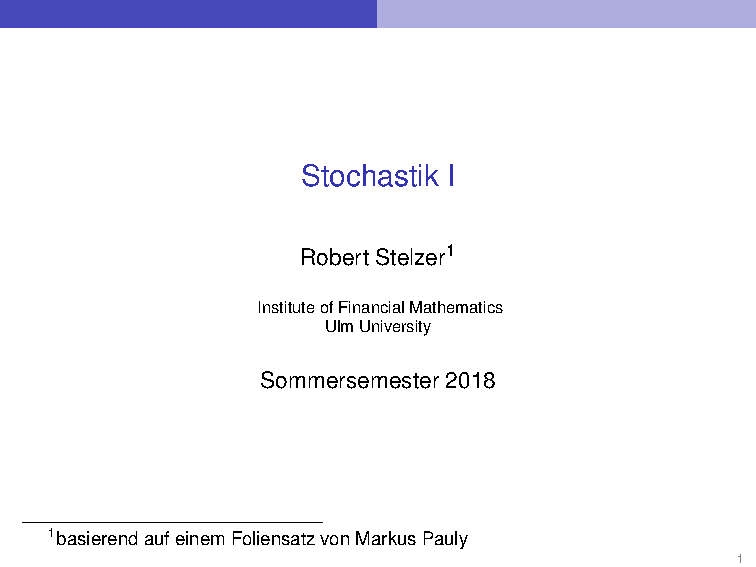
\includepdf[pages=-]{kap8.pdf}



\section{Einführung in die induktive Statistik}
\marginpar{15.Vorlesung, 14.06.2018}
\subsection{Definition}
\label{9.1}
\begin{enumerate}[label=(\roman*)]
\item Sei $(\Omega,\f)$ ein messbarer Raum, $\theta$ eine Menge (\underline{Parametermenge}) und \[\p=\brac{P_\vartheta\ \text{ Wahrscheinlichkeitsmaß auf }(\Omega,\theta):\vartheta\in\theta}\]
eine Familie von Wahrscheinlichkeitsmaßen auf $(\Omega,\f)$. Dann heißt $\raum$ ein \underline{statistisches Experiment} (SE).
\item Ist $\theta\subseteq\R^d$ für ein $d\in\N$, so spricht man von einem \underline{parametrischen Experiment/Modell}
\item Gilt $P_{\vartheta_1}\neq P_{\vartheta_2}\qf \vartheta_1,\vartheta_2\in\theta$ mit $\vartheta_1\neq\vartheta_2$, so heißt das Modell \underline{identifizierbar}
\end{enumerate}

\subsection{Annahme}
\label{9.2}
Wir nehmen stets an, dass die betrachteten SE identifizierbar sind.

\subsection{Definition}
\label{9.3}
Sei $\raum$ SE und $D$ eine Menge (\underline{Entscheidungsraum}).\begin{enumerate}[label=(\alph*)]
\item Eine Abbildung $g:\p\ra D$ heißt \underline{statistisches Funktional}
\item Sei $\mc{D}$ eine $\sigma$-Algebra auf $D$. Dann heißt eine messbare Abbildung $T:(\Omega,\f)\ra(D,\mc{D})$ \underline{(Punkt)schätzer}
\item Sei $D\subseteq\R^d$. Ein Punktschätzer T heißt \underline{erwartungstreu/unverzerrt/unbiased} für ein statischtisches Funktional $g$, falls $T\in\lp{1}(P_\vartheta)\qf \vartheta\in\theta$ und $E_\vartheta(T)=E_{P_\vartheta}(T)=g(\vartheta)=g(P_\vartheta)$
\item Für einen integrierbaren Punktschätzer $T$ heißt \[
Bias_\vartheta(T)=:=E_\vartheta(T)-g(\vartheta)\]
\underline{der Bias/die Verzerrung} von $T$ in $\vartheta$.\\
Für (quadratintegrierbare) Schätzer heißt \[
MSE_\vartheta(T):=E_\vartheta(\norm{T-g(\vartheta)}^2)\]
der \underline{mean-squared-error} von $T$ in $\vartheta$.
\end{enumerate}

\subsection{Lemma}
\label{9.4}
\[MSE_\vartheta(T)=Var_\vartheta(T)+Bias_\vartheta(T)^2\]

\subsection{Beispiel}
\label{9.5}
Sei $(\R^n,B(\R^n),\p=P^{\theta n})$ mit $P\in M_1(\R,B(\R))\quad$ ( = Menge aller Wahrscheinlichkeitsmaße auf $(\R,B(\R)))$ ein n-faches Produktmodell und $g:\p\ra M_1(\R,B(\R))=:D\\
P^\stuff\mapsto P$.\\
Dann ist das empirische Maß $T(x_1,...,x_n):=\dfrac{1}{n}\sumi\delta_{x-i}$ ein Schätzer für $g$. (Wir verzichten absichtlich auf Details zu $\mc{D}$ und zur Messbarkeit)

\subsection{Definition}
\label{9.6}
Ein SE $\raum$ heißt \underline{dominiert}, falls ein $\sigma$-endliches Maß auf $(\Omega,\f)$ existiert mit $P\ll\mu\qf P\in\p$ (i.Z. $\p\ll\mu$).\\
In einem dominierten Modell können alle $P_\vartheta$ durch Dichten bezüglich $\mu$ beschrieben werden

\subsection{Bemerkung}
\label{9.7}
\begin{enumerate}[label=(\roman*)]
\item $\mu$ kann o.B.d.A. als Wahrscheinlichkeitsmaß angenommen werden. Sonst wähle $E_i\nearrow\Omega$ mit endlichem Maß und betrachte\[
A\mapsto\tilde{\mu}(A):=\sm{i=1}\dfrac{\mu(A\cap E_i)}{2^i\mu(E_i)}\]
\item Man kann sogar zeigen: \\
Ist $\p\ll\mu, \mu\ \sigma$-endlich, so existiert eine Folge $\folge{P}{n}$ in $\p$ mit \[
\p\ll\sm{n=1}\dfrac{P_n}{2^n}\]
\item Gilt für $\p_i:=\brac{P_{i,\vartheta}:\vartheta\in\theta_i}$ f+r i=1,2 \\
$\p_i\ll\mu_i$ mit $\mu_i\ \sigma$-endlich\\
So gilt auch\[
\p_1\otimes\p_2:=\brac{P_{1,\vartheta_1}\otimes P_{2,\vartheta_2}:\vartheta\in\theta_i}\ll\mu_1\otimes\mu_2\]
\item Sei $Y=a+Z,\ a\in\R$ und $Z\sim P\in M_1\rbor[]$ fest.\\
Sei $\p:=\brac{P*\delta_a:a\in\R}$\\
Dann gilt:\\
$\p\ll\mu,\ \mu\ \sigma-endlich\LRa\p\ll\lambda$\\
\beweis
\glqq $\La$ \grqq $P*\delta_a\ll\lambda*\delta_a=\lambda$ aufgrund der Translationsinvarianz. Setze $\mu=\lambda$\\
\glqq $\Ra$ \grqq o.B.d.A $\mu$ Wahrscheinlichkeitsmaß. Sei $A\in\mc{B}(\R)$ mit\\
$0=\mu*\lambda(A)=\intr \underbrace{\mu(A-y)}_{\geq 0}\lambda(dy)$\\
$\Ra \exists y_0\in\R$ mit $\mu(A-y_0)=0\quad \lambda-$f.ü.\\
$\xRightarrow{\p\ll\mu} 0=P*\delta_{a-y_0}(A-y_0)=P\times\delta_a(A)=0\quad \forall a$\\
$\Ra \p\ll\mu*\lambda$\\
$\mu*\lambda(A)=\int \lambda(A-y)d\mu(y)=\lambda(A)\underbrace{\int d\mu(y)}_{=1}=\lambda(A)$
\end{enumerate}

\section{Suffizienz}
$X_1,...,X_n$ seien Realisierungen unabhängiger Versuchswiederholungen nach einer unbekannten Verteilung P auf $(\Omega,F)$.\\
n-faches Produktmodell: $\p=\brac{P_\vartheta^\stuff:\vartheta\in\theta}$.\\
Häufig besitzen Teile der Daten $X_1,...,X_n$ keine zusätzliche Information über das wahre $\vartheta$!\\
\textbf{Ziel:} \begin{list}{•}{}
\item Transformation der Daten ohne Informationsverlust
\item Datenkompression ohne Informationsverlust
\end{list}
Sei zum Beispiel\\
$T:(\Omega^n,\f^\stuff)\ra(\Omega_T,\f_T)$ (polnisch) eine Transformation.\\
Wenn die bedingte Verteilung ($P\in\p$ unbekannt)
\[(P_\vartheta^\stuff)^{id|T=t}\]
für alle t unabhängig von $\vartheta\in\theta$ wählbar ist, sollte $T(X_1,...,X_n)$ alle Informationen der Daten über $\theta$ enthalten.

\subsection{Beispiele}
\label{10.1}
\begin{enumerate}[label=(\roman*)]
\item Betrachte $\brc{\brac{0,1}^n,\p(\brac{0,1}^n), Binom(1,\vartheta)^\stuff}$.\\
Dann sollte die Komprimierung\\
$T:(x_1,...,x_n)\mapsto\sm[n]{i=1}x_i$ ohne Informationsverlust sein.\\
Es gilt $\forall 0\leq k\leq n$ und $\forall\brac{x_1,...,x_n}+\brac{0,1}^n$ mit $\sm[n]{i=1}X_i=K:\\
P_\vartheta^n((x_1,...,x_n)|T=K)=\dfrac{\prod\limits_{i=1}^n\vartheta^{x_i}(1-\vartheta)^{1-x_i}}{\mat{n\\K}\vartheta^K(1-\vartheta)^{n-K}}=\mat{n\\K}^{-1}$\\
Was nicht von $\vartheta$ abhängt.
\item Gegeben sei ein Produktmodell $(\Omega^n,\f^\stuff, (P_\vartheta^\stuff)_{\vartheta\in\theta})$\\
Dann sollte die Reihenfolge der Beobachtungen irrelevant sein.\\ Insbesondere sollten die Ordnungsstatistiken dieselben Informationen beinhalten wie die Daten. In der Tat kann man zeigen (siehe Skript Pauly)\\
$P_\vartheta^{\stuff\  id|(x_{(1)},...,x_{(n)})=(y_1,...,y_n)}$\\
hängt nicht von $\vartheta$ ab.\\
Da bedingte Verteilungen nicht immer existieren müssen, nutzen wir für die allgemeine Definition bedingte Erwartungswerte.
\end{enumerate}

\subsection{Definition}
\label{10.2}
Sei $(\Omega,\f,\p)$ ein statistisches Experiment.\begin{enumerate}[label=(\alph*)]
\item Eine \underline{Teil-$\sigma$-Algebra} $\tau\subseteq\f$ heißt \underline{suffizient für $\p$}, (bzw. $\vartheta$), falls für alle $A\subset\f$ eine von $\vartheta$ unabhängige Version $E_\bullet(1_a|\tau)$ des bedingten Erwartungswertes $E_{P_\vartheta}(1_A|\tau)$ existiert
\item Sei $T:(\Omega,\f)\ra(\Omega',\f')$ eine Statistik.\\
T heißt \underline{suffizient für $\p$}, falls $\tau=T^{-1}(\f')(=\sigma(T))$ suffizient ist.\\
\end{enumerate}

\textbf{Interpretation:}
Wir werden sehen:\begin{enumerate}
\item Bei der Suffizienz enhält das SE $(\Omega, \tau, \brac{P_{\vartheta|\tau}}_{\vartheta\in\theta})$ \\genau soviel Information über $\vartheta$ wie das Ausgangsexperiment
\item Die Reduktion der Daten wird einen Effizienzgewinn (niedrigere Varianz) mit sich bringen
\end{enumerate}
d.h. Suffizienz ist sozusagen \glqq Datenredutkion ohne Informationsverlust \grqq.


\subsection{Lemma}
\label{10.3}
Sei $X$ eine Statistik auf $(\Omega,\f),\ X\in\lp{1}(P_\vartheta)\quad \forall\vartheta\in\theta$ und $\tau\subseteq\f$ suffizient.\\
Dann existiert eine Version $E_\bullet(X|\tau)$ von $E_{P_\vartheta}(X|\tau)$ die unabhängig von $\vartheta$ ist.\\
\beweis
Offensichtlich für $X=1_A\quad\forall A\in\f$. Dann maßtheoretische Induktion.\QED

\subsection{Bemerkung (Extremfälle)}
\label{10.4}
\begin{list}{•}{}
\item Ist $T^{-1}(\f')=\f$, so ist $T$ suffizient.
\item $\tau=\brac{\emptyset,\Omega}:$ Suffizienz hieße $E_\vartheta(1_A|\tau)=P_\vartheta(A)\quad\forall A\in\f$ wäre unabhängig von $\vartheta$. Das ist nur in trivialen Fällen möglich.
$\Ra$ suffiziente $\sigma$-Algebren/Statistiken können nicht \glqq zu klein\grqq\ sein
\end{list}

\subsection{Lemma}
\label{10.5} Sei $(\Omega,\f,\p)$ ein statistisches Experiment.\begin{enumerate}[label=(\alph*)]
\item T ist suffizient $\LRa \forall A\in\f$ existiert eine von $P_\vartheta$ unabhängige Version $E_\bullet(1_A|T=\cdot)$ von $E_{P_\vartheta}(1_A|T=\cdot).$
\item Existiert eine von $P_\vartheta\in\p$ unabhängige Version \\
$K(t,\cdot)=P^{id|T=t}$\\
so ist T suffizient für $\p$.
\end{enumerate}

\subsection{Satz (Rao-Blackwell)}
\label{10.6}
Sei $(\Omega,\f,\p)$ ein SE und S ein erwartungstreuer Schätzer für $g(\vartheta)$. Weiter sei $\tau$ suffizient und $h:=E_\bullet(S|\tau)$. Dann gilt:\begin{enumerate}[label=(\roman*)]
\item h ist $\tau$-messbarer erwartungstreuer Schätzer für $g(\nu)$
\item $MSE_\vartheta(h)=Var_\vartheta(h)\leq Var_\vartheta(S)=MSE_\vartheta(S)\qf\vartheta\in\theta$ mit \grqq$=$\grqq, falls \\
$E_\vartheta(S|\tau)=S P_\vartheta-f.s.\forall\vartheta$\\
\beweis
\hyperref[6.2]{Bedingte Jensensche Ungleichung}\QED
\end{enumerate}

\subsection{Satz (Neyman-Kriterium)}
\label{10.7}
Sei $(\Omega,\f,\p)$ ein statistisches Experiment, $\p\ll\mu$ mit $\mu\ \sigma$-endlich. Für eine Statistik $T:\Omega\ra\Omega'$ sind äquivalent:\begin{enumerate}[label=(\alph*)]
\item $T$ ist $\p$-suffizient
\item $\exists \f'$- messbare Funktionen $g_p:\Omega'\ra [0,\infty)$ und\\ eine $\f$-messbare Funktion $h:\Omega\ra [0,\infty)$ mit \[\dfrac{dP}{d\mu}=(g_p\circ T)\cdot h\quad\forall P\in\p$ $(\mu-\text{f.ü.})\] 
\end{enumerate}

\subsection{Bemerkung}
\label{10.8}
\marginpar{16.Vorlesung, 18.06.2018}
Es genügt in b) $\dfrac{dP}{d\mu}=g_P\circ T$ zu fordern (ersetzte $\mu$ durch $\widehat{\mu}$ mit $\widehat{\mu}(A)=\int\limits_Ahd\mu$\\
\beweis
Wir zeigen nur den diskreten Fall.\\
\glqq $\Ra$ \grqq $\forall x\in\Omega,\ \forall P\in\p\ \exists$ Funktionen $f_x$ mit \[
P(\brac{x}|T=t)=f_x(t)\quad P^T-f.s.\quad(\text{d.h. auf P(T=t)>0)}\]
Setze $h(x)=f_x(T(x))$ und $g_P(t)=P(T=t)$, so folgt \\
$P(\brac{x})=P(\brac{x}\cap\brac{T=T(x)})=P(\brac{x}|T=T(x))P(T=T(x))\\
=h(x)g_P(T(x))$\\
(Gilt offensichtlich auch für $P(T=T(x))=0$.\\
\glqq $\La$ \grqq Es gilt\\
\[P(\brac{x}|T=t)=\dfrac{P(\brac{x}\cap\brac{T=t})}{P(T=t)}\quad P^T-f.s \hfill(10.1)\]\[
P(\brac{x}\cap\brac{T=t})=\begin{cases}
0, & \text{ falls }T(x)\neq t\\
P(\brac{x}) & \text{ sonst}
\end{cases}\hfill (10.2)\]
Sei also $T(x)=t$ (sonst klar), dann gilt\[
P(T=t)=\sm[]{z:T(z)=t}P(\brac{z})\hfill(10.3)\]
Einsetzen von b) in (10.2) und (10.3) liefert für (10.1)\[
P(\brac{x}|T=t)=\dfrac{g_P(T(x))h(x)}{\sm[]{z:T(z)=t}g_P(T(z))h(z)}=\dfrac{h(x)}{\sm[]{z:T(z)=t}h(z)}\]
was von P unabhängig ist.\QED

\subsection{Korollar}
\label{10.9}
Sei $(\Omega,\f,\p)$ SE, $\p\ll\mu,\ \mu\ \sigma$-endlich und $\tau\subseteq\f\ \sigma$-Algebra. Dann sind äquivalent:\begin{enumerate}[label=(\alph*)]
\item $\tau$ ist $\p$-suffizient
\item $\forall P\in\p\ \exists \tau$-messbare Funkion $f_P:\Omega\ra\R$ und eine von $P\in\p$ unabhängige $\f$-messbare Abbildung $h:\Omega\ra\R$ mit \[\dfrac{dP}{d\mu}=f_P\cdot h\quad \mu-f.s.\]
\end{enumerate}

\subsection{Korollar}
\label{10.10}
Sei $(\Omega,\f,\p)$ SE, $\p\ll\mu, \mu\ \sigma$-endlich und $\tau$ eine suffiziente $\sigma$-Algebra. Dann ist jede $\sigma$-Algebra $\tau'$ mit $\tau\subseteq\tau'\subseteq\f$ ebenfalls suffizient.\\
\beweis
In Korollar 10.9 ist $f_p\ \tau$- und damit $\tau'$-mmessbar.\QED

\subsection{Korollar}
\label{10.11}
Seien $(\Omega_i,\f_i,\p_i), i=1,2$ dominierte statistische Experimente und $\tau_i\subseteq\f_i$ seien suffiziente $\sigma$-Algebren. \\
Dann ist $\tau_1\otimes\tau_2=\sigma(\tau_1\times\tau_2)$ suffizient für \\
$\p_1\otimes\p_2:=\brac{P_1\otimes P_2:P_i\in\p_i, i=1,2}$.\\
\beweis
\[\dfrac{dP_1\otimes P_2}{d\mu_1\otimes\mu_2}(x,y)=\dfrac{dP_1}{d\mu_1}(x)\dfrac{dP_2}{d\mu_2}(y)=\underbrace{\overbrace{f_{P_1}(x)}^{\tau_1-messbar}\overbrace{f_{P_2}(y)}^{\tau_2-messbar}}_{\tau_1\otimes\tau_2-messbar}\cdot\underbrace{h_1(x)h_2(y)}_{h(x,y)}\]
Mit Korollar 10.9 folgt die Behauptung\QED

\subsection{Korollar}
\label{10.12}
Sei $(\Omega,\f,\p)$ dominierte SE und $T:\Omega\ra\Omega'$, $f:\Omega'\ra\Omega''$ Statistiken.\\
Ist $T'=f\circ t$ suffizient, so ist $T$ suffizient.\\
\beweis
Folgt aus Korollar 10.11, da $\sigma(T)\supseteq\sigma(f\circ T)$.\QED

\subsection{Definition}
\label{10.13}
Sei $(\Omega,\f,\p)$ ein SE. $\p=\brac{P_\vartheta:\vartheta\in\theta}$ heißt \underline{Exponentialfamilie}, falls $\mu\ \sigma$-endlich existiert mit $\p\ll\mu$ und es Funktionen $g_1,...,g_k:\theta\ra\R$ für $k\in\N$ sowie Statistiken $T_1,...,T_k:\Omega\ra\R$ gibt mit \[
\dfrac{dP_\vartheta}{d\mu}=C(\vartheta)\exp\brc{\sm[k]{i=1}g_i(\vartheta)T_i(x)}h(x)\hfill(10.4)\]
wobei $h:\Omega\ra\R$ messbar und\[
C(\vartheta)=\brc{\int\limits_\Omega\exp\brc{\sm[k]{i=1}g_i(\vartheta)T_i(x)}h(x)d\mu(x)}^{-1}\]

\subsection{Satz}
\label{10.14}
Für eine Exponentialfamilie $\p$ wie in (10.4) ist $(T_1,T_2,...,T_k)$ eine suffiziente Statistik.\\
\beweis
Nutze \hyperref[10.7]{Theorem 10.7} mit $\\
g_P:\R^k\ra\R\\
(x_1,...,x_n)\mapsto\exp\brc{\sm[k]{i=1}g_i(\vartheta)x_i}$\QED

\subsection{Beispiel (Suffizienz und Exponentialfamilien)}
\label{10.15}
\begin{enumerate}[label=(\alph*)]
\item $\theta\in(0,1), P_\vartheta=Binom(n,\vartheta), \mu=\sm[]{n\in\N_0}\delta_n$ (Zählmaß)\\
Dann gilt
\begin{align}
P_\vartheta(\brac{x}) & = \mat{n\\k}\vartheta^x(1-\vartheta)^{n-x}1_{\brac{0,...,n}}(x)\\
& = \underbrace{(1-\vartheta) ^n}_{C(\vartheta)}\exp\bigg(\underbrace{x}_{T_1(x)}\underbrace{log\dfrac{\vartheta}{1-\vartheta}}_{g_1(\vartheta)}\bigg)\underbrace{\mat{n\\x}1_{\brac{0,...,n}}(x)}_{h(x)}
\end{align}
Somit liegt eine Exponentialfamilie vor und $T(x)=x$ ist suffizient für $\p=\brac{Binom(n,\vartheta:\vartheta\in(0,1)}$
\item Offensichtlich sind Produkte von Exponentialfamilien wieder\\ Exponentialfamilien, z.B. betrachte a) mit $n=1, \theta=(0,1)$, und davon das N-fache Produktexperiment. Dann gilt: $P_\vartheta=Binom(1,\vartheta)^{\otimes N}\\
P_\vartheta(\brac{x})=\vartheta^{\sm[N]{i=1}x_i}(1-\vartheta)^{N-\sm[N]{i=1}x_i}\\
=(\underbrace{1-\vartheta}_{C(\vartheta)})^N\exp\bigg(\underbrace{\sm[N]{i=1}x_i}_{T_1(x)}\underbrace{log\brc{\dfrac{\vartheta}{1-\vartheta}}}_{g_1(\vartheta)}\bigg)\underbrace{1_{\brac{0,1}}(x)}_{h(x)}$\\
Somit ist $T(x)=\sm[N]{i=1}x_i$ suffizient.
\item Sei $\vartheta=(\mu,\sigma^2)\in\theta=\R\times\R^+\setminus\brac{0},\ \p_\vartheta=N(\mu,\sigma^2)^\stuff$\\
und $\mu=\lambda^n$. Dann gilt \[
\dfrac{dP_\vartheta}{d\mu}(x_1,...,x_n)=\underbrace{\brc{\dfrac{1}{\sqrt{2\pi\sigma^2}}}^ne^{-\dfrac{n\mu^2}{2\sigma^2}}}_{C(\vartheta)}\exp\\bigg(\underbrace{\dfrac{\mu}{\sigma^2}}_{g_1(\vartheta)}\underbrace{\sm[N]{i=1}x_i}_{h(x)}-\underbrace{\dfrac{1}{2\varsigma^2}}_{g_2(\vartheta)}\underbrace{\sm[N]{i=1}x_i^2}_{T_2(i)}\bigg)
\]
Also liegt eine Exponentialfamilie mit $k=2$ und suffiziente Statistik\[
T(x)=(T_1(x),T_2(x))=\brc{\sm[N]{i=1}x_i,\sm[N]{i=1}x_i^2}\]
vor.
\marginpar{17.Vorlesung, 21.06.2018} \\
Leicht sieht man, dass eine messbare Abbildung $f:\R^2\ra\R^2$ existiert, so dass 
\[f\brc{\overline{x_n},\dfrac{1}{n-1}\sm[n]{i=1}(x_i-\overline{x_n})^2}=T(x)\] 
Aus Korollar 10.12 folgt somit, dass \\
$\brc{\overline{x_n},\dfrac{1}{n-1}\sm[n]{i=1}(x_i-\overline{x_n})^2}$(ebenfalls  suffizient für $\mc{P}=\brac{N(\mu,\sigma^2)^\stuff:\mu\in\R,\sigma^2>0}$ ist.
\end{enumerate}





\subsection{Beispiel (Suffizienz ohne Exponentialfamilie)}
\label{10.16} 
Sei $\mc{U}_{(a,b)}=\dfrac{\lambda\vert_{(a,b)}}{b-a}$ die Gleichverteilung auf $(a,b), b>a$. Sei \\
$\mc{P}=\brac{\mc{U}_{(a,b)}^\stuff:\vartheta=(a,b)\in\R^2, a<b}$. Aus \hyperref[10.13]{Definition 10.13} folgt sofort, dass in einer Exponentialfamilie gilt\[
P_{\vartheta_1}\sim P_{\vartheta_2}\forall\vartheta_1,\vartheta_2\in\theta\]
Somit ist $\mc{P}$ sicher keine Exponentialfamilie. Aber $T(x)=\brc{\min\limits_{i=1,...,n}x_i,\max\limits_{i=1,...,n}x_i}$ ist suffizient, denn:\[
\dfrac{dP_\vartheta}{d\lambda^n}(x)=\dfrac{1}{(b-a)^n}\prod\limits_{i=1}^n1_{(a,b)}(x_i)=\dfrac{1}{(b-a)^n}1_{(a,\infty)}(\min x_i)1_{(-\infty,b)}(\max x_i)
\]
womit das Neyman-Kriterium erfüllt ist.

\section{Vollständigkeit und UMVU Schätzer}
Der Satz von Rao-Blackwell bietet ein Verfahren zur Verbesserung erwartungstreuer Schätzer durch Nutzung sufizienter $\sigma$-Algebren an. Wir werden nun versuchen, optimale Schätzer zu erhalten.

\subsection{Definition}
\label{11.1}
Sei $(\Omega,\f,\p)$ ein SE.\begin{enumerate}[label=(\alph*)]
\item Ein statistisches Funktional $g:\mc{P}\ra\R$ heißt \underline{erwartungstreu schätzbar}, falls eine erwartungstreuer Punktschätzer für g existiert.
\item Sei g erwartungstreu schätzbar. Dann heißt ein erwartungstreuer Schätzer $h^*:\Omega\ra\R$\\
\underline{gleichmäßig bester erwartungstreuer (UMVU) Schätzer} für g, falls $Var_\vartheta(h^*)<\infty\forall\vartheta\in\theta$ und\[
Var_{\vartheta}(h^*)=\min\limits_{\substack{\text{h erw.treu}\\\text{für g}}}Var_\vartheta(h)\quad\forall\vartheta\in\Theta\] gilt.
\end{enumerate}

\subsection{Bemerkung}
\begin{enumerate}[label=(\roman*)]
\item Statistische Funktionale müssen nicht erwartungstreu schätzbar sein.
\item Konvexkombinationen erwartungstreuer Schätzer sind erwartungstreu
\item Die Varianz kann man prinzipiell in der folgenden Theorie durch sogenannte Verlustfunktionen ersetzen
\end{enumerate}

\subsection{Satz (Eindeutigkeit)}
\label{11.3}
Seien $h_1,h_2$ UMVUE für g. Dann gilt \[
P_\vartheta(h_1\neq h_2)=0\quad\forall\vartheta\in\theta\]
\beweis Siehe elementare Wahrscheinlichkeitsrechnung und Statistik\QED

\subsection{Satz (Raosche Kovarianzmethode)}
\label{11.4}
Sei $h^*$ erwartungstreu für g und $Var_\vartheta(h^*)<\infty\quad\forall\vartheta\in\theta$. Dann sind äquivalent:\begin{enumerate}[label=(\alph*)]
\item $h^*$ ist UMVUE
\item $\forall$ Nullschätzer d, d.h. Schätzer mit $E_\vartheta(d)=0$ und $Var_\vartheta(d)<\infty\quad\forall\vartheta$, gilt $Cov(h^*,d)=0\quad\forall\vartheta$
\end{enumerate}
\beweis
\glqq $\La$\grqq\\
Sei $h$ erwartungstreu mit $Var_\vartheta(h)<\infty$. Dann $d=h-h^*$ Nullschätzer und\\
$Var_\vartheta(h)=Var_\vartheta(d+h*)=\underbrace{Var_\vartheta(d)}_{\geq0}+Var_\vartheta(h^*)+2\underbrace{Cov(h^*,d)}_{=0}\geq Var_\vartheta(h^*)\\
\Ra h^*$ ist UMVUE.\\
\glqq $\Ra$ \grqq\\
Offenbar ist $d_t:=h^*+td$ erwartungstreu $\forall f\in\R$. \\
Somit $ Var_\vartheta(h^*)\leq Var_\vartheta(d_t)=Var_\vartheta(h^*)+t^2Var_\vartheta(d)+2tCov_\vartheta(d,h^*)$\\
Die rechte Seite hat ein Minimum in $t=0$ (und ist $\geq 0$)\\
$\Ra Cov_\vartheta(d,h^*)=0$\QED

\subsection{Definition (Vollständige $\sigma$-Algebra)}
\label{11.5}
Sei $\rraum$ SE.\begin{enumerate}[label=(\alph*)]
\item Eine $\sigma$-Algebra $\tau\subseteq\f$ heißt \underline{vollständig (für $\p$)}, falls gilt:\\
$\forall f:\Omega\ra\R, \tau-messbar, f\in\lp{1}P_\vartheta)\quad \forall\vartheta$ mit \\
$E\vartheta(f)=0\quad\forall\vartheta$ ist\[
f=0\quad P_\vartheta\vert_\tau-f.s.\quad\forall\vartheta\]
\item Eine Statistik $T:(\Omega,\f)\ra(\Omega',\f')$ heißt \underline{vollständig}, falls  $T^{-1}(\f')=\sigma(T)$ vollständig ist.
\item Eine $\sigma$-Algebra $\tau\subseteq\f$ (eine Statistik T) heißt \underline{beschränkt vollständig}, falls \hyperref[11.1]{(11.1)} für alle beschränkten messbaren f gilt.
\end{enumerate}
Vollständigkeit bedeutet also, dass alle $\tau$-messbaren Nullschätzer trivial (also f.s. identisch Null) sind. Vollständige $\sigma$-Algebren sind also eher klein.

\subsection{Bemerkung}
\label{11.6}
\begin{enumerate}[label=(\roman*)]
\item $T:(\Omega,\f)\ra(\Omega',\f')$ ist genau dann vollständig, wenn $\forall h:\Omega'\ra\R$ messbar mit $h\circ T\in\lp{1}(P_\vartheta)$ und $E_{P_\vartheta}(h\circ T)=0\quad\forall\vartheta\in\theta$ folgt $h\circ T\equiv0\quad P_\vartheta-f.s.$
\item Ein Resultat Bahadour:\\
Ist T suffizient und beschränkt vollständig für $\mc{P}$, so existiert für alle suffizienten S eine messbare Abbildung $\varphi$ mit $T=\varphi\circ S$.\\
Somit gilt $\sigma(T)\subseteq\sigma(S)$.\\
Man spricht von \underline{Minimalsuffizienz} für T und T ergibt sozusagen eine maximal mögliche Datenkompression ohne Informationsverlust.
\end{enumerate}

\subsection{Beispiel}
\label{11.7}\begin{enumerate}[label=(\alph*)]
\item Sei $\mc{P}=\brac{P\in M_1\rbor[]:P(A)=P(-A)\quad\forall A\in\mc{B}(\R)}$.\\
Dann ist $\mc{B}(\R)$ nicht vollständig für $\mc{P}$, denn \[
\intr \underbrace{1_{(0,\infty)}-1_{(-\infty,0)}}_{\neq0}dP=0\quad\forall P\in\mc{P}\]
\item Sei $\mc{P}=\brac{Binom(1,\vartheta)^\stuff:\vartheta\in(0,1)}$ und \\
$T:\brac{0,1}^n\ra\brac{0,...,n}$ mit $(x_1,...,x_n)\mapsto\sm[n]{i=1}x_i$. Dann ist T vollständig für $\mc{P}$.
\end{enumerate}
\beweis
Betrachte $h:\brac{0,1,...,n}\ra\R$ mit $E_{P_\vartheta}(h\circ T)=0\quad\forall \vartheta\\
\Ra 0=\sm[n]{k=0}h(k)\mat{n\\k}\vartheta^k(1-\vartheta)^{(n-k)}\\
= (1-\vartheta)^n\sm[n]{k=0}h(k)\bigg(\underbrace{\dfrac{\vartheta}{1-\vartheta}}_{=:\varsigma\in(0,\infty)}\bigg)^k\\
\Ra\sm[n]{k=0}h(k)\mat{n\\k}\varsigma^k=0\quad\forall\varsigma\in(0,\infty)\\
\Ra$ Dies muss das Nullpolynom in $\varsigma$ sein\\
$\Ra h(k)=0\quad \forall k\in\N_0$






\subsection{Satz (Lehmann-Scheffe)}
\label{11.8}
\marginpar{18.Vorlesung, 28.06.2018}
Sei $g:\mc{P}\ra\R$ erwartungstreu schätzbar und h ein erwartungstreuer Schätzer für $g$ mit $Var_\vartheta(h)<\infty\quad\forall\vartheta$. Dann gilt\begin{enumerate}[label=(\alph*)]
\item Ist $\tau\subseteq\f$ suffizient und vollständig für $\mc{P}$, dann ist \[
h^*:=E_\bullet(h|z)\]
der (f.s. eindeutige) UMVUE für $g$.
\item Ist $T:\Omega\ra\Omega'$ eine suffiziente und vollständige Statistik, dann ist $f^*\circ T$ mit $f^*(t)=E_\bullet(h|T=t)$ der (f.s. eindeutige) UMVUE für $g$.
\end{enumerate}
\beweis
b) folgt offensichtlich aus a)\\
Ad a)\\
Offensichtlich ist $h^*$ unverzerrt. Sei $\tilde{h}$ erwartungstreu mit $Var_\vartheta(\tilde{h})<\infty$. Mit Rao-Blackwell gilt \[
Var_\vartheta(\tilde{h})\geq Var_\vartheta(E_\bullet(\tilde{h}|\tau))\quad\forall\vartheta\hfill(*)\]
Aus der Erwartungstreue folgt \[
E_\vartheta(\underbrace{h^*-E_\bullet(\tilde{h}|z)}_{\tau-messbar})=g(\vartheta)-g(\vartheta)=0\]
Da $\tau$ vollständig ist, folgt $h^*=E_\bullet(\tilde{h}|\tau)\quad P_\vartheta-f.s.\quad\forall\vartheta$. Nun folgt aus $(*)$ die Varianzminimalität. Die Eindeutigkeit folgt aus \hyperref[11.3]{Satz 11.3}.\QED


\subsection{Beispiel}
\label{11.9}
Aus den Beispielen \hyperref[11.7]{11.7 b)} und \hyperref[10.15]{10.15 b)} folgt, dass $T(x)=\sumi x_i$ suffizient und vollständig ist für $\brac{Binom(1,\vartheta)^\stuff:\vartheta\in(0,1)}$\\
Erwartungstreuer Schätzer ist $\widehat{\vartheta}(x)=\dfrac{1}{n}\sumi x_i$. Dieser ist offensichtlich $\sigma(T)$-messbar. Mit \hyperref[11.8]{Lehmann-Scheffe} ist $\widehat{\vartheta}$ also UMVUE für $\vartheta$.\\
\\
Hat man eine suffiziente und vollständige Statistik T, so kann man folgende zwei Möglichkeiten nutzen, um einen UMVUE zu finden:\begin{enumerate}[label=(\roman*)]
\item Finde einen beliebigen erwartungstreuen Schätzer h und berechne\\ $h^*=E_\bullet(h|T)$
\item Finde eine messbare Funktion f mit \[E_\vartheta(f\circ T)=g(\vartheta)\quad\forall\vartheta\in\theta\]
\end{enumerate}

\subsection{Beispiel}
\label{11.10}
Sei $\mc{P}=\brac{P_b^\stuff:P_b=\mc{U}_{(0,b)},b>0}$. Dann ist $T(x)=\max\limits_{1\leq i\leq n}x_i$ suffizient und vollständig.\\
\beweis
Suffizienz analog zu \hyperref[10.16]{Beispiel 10.16}.\\
Es gilt $P_b^\stuff(T\leq t)=P(x_1\leq t)^n=\brc{\dfrac{t}{n}}^b\quad\forall 0\leq t\leq b$\\
Sei nun $b>0$ und $f$ so, dass $f\circ T\in\lp{1}(P_b)\quad\forall b$ und \\
$0=E_b(f\circ T)=\intr f(t)d(P_b^\stuff)^T=\int\limits_0^bf(t)\dfrac{nt^{n-1}}{b^n}dt$\\Zerlege $f=f^+-f^-$ in Positiv- und Negativteil:\[
\int\limits_0^bf^+(t)t^{n-1}dt=\int\limits_0^bf^-(t)t^{n-1}dt\quad\forall b>0\]
Betrachte die Maße $\mu^+$ und $\mu^-$ auf $B((0,\infty))$ mit \\
$\mu^+(B)=\int\limits_Bf^+(t)t^{n-1}dt,\ \mu^-(B)=\int\limits_Bf^-(t)t^{n-1}dt.$\\
Mit dem Eindeutigkeitssatz für Maße gilt $\mu^+=\mu^-$ und beides sind $\sigma$-endliche Maße.\\
Aus Radon-Nikodym (f.ü. Eindeutigkeit der Dichte) folgt \\
$\dfrac{d\mu^+}{d\lambda}=\dfrac{d\mu^-}{d\lambda}\quad\lambda-\text{f.ü.}\\
\Ra f^+=f^-\quad \lambda$-f.ü. $\Ra f=0\quad\lambda$-f.ü. und damit $(P_b^\stuff)^T-f.s.\quad\forall b>0$.\\
Mit \hyperref[11.6]{Bemerkung 11.6 (i)} folgt die Behauptung.\QED

$h(x)=\dfrac{n+1}{n}\max\limits_{1\leq i\leq n}x_i$ ist UMVUE, da \[E_\vartheta(h(x))=\dfrac{n+1}{n}\int\limits_0^bt\dfrac{nt^{n-1}}{b^n}dt=\dfrac{t^{n+1}}{b^n}\Bigg\vert_0^b=b\]\QED

Wir wenden uns nun wieder Exponentialfamilien zu, Sei \[
\mc{P}=\brac{P_\vartheta:\vartheta\in\theta}\ll\mu\quad(\mu-\sigma-endlich)\]
von der Form \[
\dfrac{dP_\vartheta}{d\mu}(x)=C(\vartheta)\exp \brc{\sm[k]{i=1}g_i(\vartheta)T_i(x)}h(x)\]
Dann heißt die Menge \[
\Xi^*:=\brac{s\in\R^k:\int\limits_\Omega exp\brc{\sm[k]{i=1}s_iT_i)}d\mu}\]
\underline{natürlicher Parameterraum} der Exponentialfamilie.
Offensichtlich gelten:\begin{list}{•}{}
\item $\Xi:=\brac{(g_1(\vartheta),...,g_n(\vartheta)):\vartheta\in\theta}\subseteq\Xi^*$
\item $\dfrac{dQ_s}{d\mu}:=\tilde{C}(s)\exp\brc{\sm[k]{i=1}s_iT_i(x)}h(x)$ definiert eine Exponentialfamilie $\brac{Q_s:s\in\Xi^*}$ in \underline{natürlicher Parametrisierung} mit \[\tilde{C}(s)=\dfrac{1}{\int\limits_\Omega\exp\brc{\sm[k]{i=1}s_iT_i(x)}h(x)\mu(dx)}\]
\end{list} 

\subsection{Lemma (Momente bei Exponentialfamilien)}
\label{11.11}

Sei $\rraum$ SE mit $\mc{P}$ Exponentialfamilie in natürlicher Parametrisierung.
\begin{enumerate}[label=(\alph*)]
\item Ist $s\in\Xi^*$ so existieren unter $Q_s$ für $T_1,...,T_k$ Momente beliebiger\\
Ordnung, d.h. $\forall (\mu_1,...,\mu_n)\in(\N_0)^k$ gilt $\prod\limits_{j=1}^kT_j^{\mu_j}\in\lp{1}(Q_s)$ und
\[\underbrace{\int\limits_\Omega\prod\limits_{j=1}^kT_j^{\mu j}dQ_s}_{E_{Q_s}(T|...)}=\tilde{C}(s)\dfrac{\partial^{\mu_1+...+\mu_k}}{{\partial s_1^{\mu_1}\partial s_2^{\mu_2}...\partial s_k^{\mu_k}}}\int\limits_\Omega e^{\langle s,T\rangle}hd\mu\]
\item Ist $\varphi:\Omega\ra\R$ messbar und beschränkt, so gilt \begin{align}
\dfrac{\partial}{\partial s_i}E_{Q_s}(\varphi) & = E_{Q_s}(\varphi T_i)-E_{Q_s}(\varphi) E_{Q_s}(T_i)\\
& = Cov_{Q_s}(\varphi,T_i)
\end{align} 
\item $\dfrac{\partial}{\partial_{s_i}}\tilde{C}(s)=-\tilde{C}(s)E_{Q_s}(T_i)$
\end{enumerate}
\beweis
\marginpar{19.Vorlesung, 02.07.2018}
\begin{enumerate}[label=(\alph*)]
\item Mittels fourieranalytischer Methoden zeigt man, dass \[
z\mapsto\int e^{\langle z,T\rangle} hd\mu=:\beta(z)\]
beliebig oft differenzierbar ist und Integration und Differentiation vertauscht werden können.\\

\underline{Intuition:} Sei $hd\mu=dP$ Wahrscheinlichkeitsmaß und es stelle $P^T$ die Verteilung von T unter $P^T$ dar. Dann \[
\int\limits_\Omega e^{\langle z,T\rangle}P^T(dt)=\varphi_T(z)\quad z\in\C\]
Momente bis zur Ordnung $\gamma$ existieren für $T_j$ falls $T\in\lp{\gamma}(P)$.\hfill(*)\\
\hyperref[4.14]{Satz 4.14} liefert $\gamma$-te Momente von T als Ableitung der charakteristischen Funktion.\\
Nun ersetzt die Bedingung $s\in\Xi^*$ in gewisser Weise Bedingung (*) und erlaubt wetergehend die Existenz aller Momente.

$\tilde{C}(S)\dfrac{\partial^{\mu_1+...+\mu_k}}{{\partial s_1^{\mu_1}\partial s_2^{\mu_2}...\partial s_k^{\mu_k}}}\int\limits_\Omega e^{\overbrace{\langle s,T\rangle}^{\sm[k]{i=1}s_iT_i}}d\mu=\int\limits_\Omega\prod\limits_{j=1}^kT_j^{\mu_j}\underbrace{e^{\langle s,T\rangle}\tilde{C}(s)h(x)d\mu(x)}_{dQs}$
\item Setze $\tilde{\beta}(s)=\int\limits_\Omega e^{\langle s,T\rangle}\underbrace{h\varphi}_{\tilde{h}}d\mu$.\\
Dann gilt \[
E_{Q_s}(\varphi)=\int\limits_\Omega\varphi dQ_s=\int\limits_\Omega\varphi e^{\langle s,T\rangle}\tilde{C}(s)hd\mu=\tilde{C}(s)\tilde{\beta}(s)\]
und damit\\
$\dfrac{\partial}{\partial s_i} E_{Q_s}(\varphi)=\tilde{C}(s)\dfrac{\partial}{\partial s_i}\tilde\beta(s)+\tilde\beta(s)\dfrac{\partial}{\partial s_i}\tilde C(s)\\
\xlongequal{a),c)}\underbrace{\tilde{C}(s)\int\limits_\Omega T_ie^{\langle s,T\rangle}\varphi hd\mu}_{E_{Q_s}(\varphi T_i}-\underbrace{\tilde\beta(s)\tilde C(s)}_{E_{Q_s}(\varphi)}E_{Q_s}(T_i)$
\item Es gilt $\tilde{C}(s)=\dfrac{1}{\beta(s)}\\
\Ra\dfrac{\partial}{\partial s_i}\tilde{C}(s)=-\dfrac{1}{\beta (s)^2}\dfrac{\partial}{\partial s_i}\beta(s)=-\dfrac{1}{\beta(s)^2}\int\limits_\Omega T_ie^{\langle s,T\rangle}h(x)d\mu(x)\\
=-\dfrac{1}{\beta(s)}\underbrace{\int\limits_\Omega T_i(x)\underbrace{e^{\langle s,T(x)\rangle}\tilde{C}(s)h(x)d\mu(x)}_{dQs}}_{E_{Q_s}(T_i)}$\QED

\end{enumerate}


\subsection{Definition}
\label{11.12}
Sei $\vartheta$ ein Maß auf $\R^k$, dann heißt\[
L_\vartheta:y\mapsto\int\limits_{\R^k}e^{\langle y,x\rangle} d\vartheta(x), \R^k\ra [0,\infty]\]
die \underline{Laplacetransformierte} oder \underline{momenterzeugende Funktion} von $\vartheta$. $I_\vartheta:=\brac{y\in\R^k:L_\vartheta(y)<\infty}$

\subsection{Satz (Eindeutigkeitssatz)}
\label{11.13}
Seien $\vartheta_1,\vartheta_2$ Maße auf $\R^k$ und $\mc{U}\neq\emptyset$ offene Menge mit $\mc{U}\subset I_{\vartheta_1}$ und $\mc{U}\subset I_{\vartheta_2}.$ Gilt \[
L_{\vartheta_1}(y)=L_{\vartheta_2}(y)\qf y\in\mc{U}\]
so ist $\vartheta_1=\vartheta_2$. (Ähnlich dem Eindeutigkeitssatz für charakteristische Funktionen).\\
\beweis
Göttliche Eingebung

\subsection{Satz}
\label{11.14}
Sei $\p$ eine Exponentialfamilie. Hat der Parameterraum \\
$\Xi=\brac{(g_1(\vartheta),...,g_k(\vartheta)):\vartheta\in\theta}\subseteq\R^k$ nichtleeres Inneres, d.h. $\Xi\neq\emptyset$, dann ist $T=(T_1,...,T_k)$ vollständig für $\p$\\
\beweis
O.b.d.A. h=1 (sonst betrachte $h\mu$ statt $\mu$).\\
Sei $f:\R^k\ra\R$ mit $f\circ T \in\lp{1}(P\vartheta)\qf\vartheta$ und \\
$\int f\circ TdP\vartheta=0\qf\vartheta\in\theta\hfill(*)$\\
z.z. nach \hyperref[11.6]{Bemerkung 11.6 (i)}: $f\circ T=0\quad P\vartheta-f.s.\qf\vartheta\in\Theta\\
\xRightarrow{(*)}C(\vartheta)\int\limits_\Omega f\circ T\exp\brc{\sm[k]{i=1}g_i(\vartheta)T_i}d\mu=0\qf\vartheta\in\theta\hfill(**)$\\
Setze $\mu^T=\mu\circ T^{-1}$\\
Dann gilt für $(**)$\[
C(\vartheta)\int\limits_{\R^k}f(t)\exp\brc{\sm[k]{i=1}g_i(\vartheta)t}d\mu^T=0\qf\vartheta\in\theta\hfill(***)
\]
Zerlege $f=f^++f^-$ und definiere Maße $\mu^-,\mu^+$ auf $\rbor[k]$ durch\[
\dfrac{d\mu^{\pm}}{d\mu^T}=f^{\pm}\]\[
\int\limits_{\R^k}e^{\langle s,T\rangle} d\mu^+(t)=\int\limits_{\R^k}e^{\langle s,t\rangle}d\mu^-(t)\qf s\in\Xi.
\]
Mit \hyperref[11.13]{Satz 11.13} folgt $\mu^+=\mu^-\\
\Ra f^+=f^-\quad\mu^T-$f.ü. (Eindeutigkeitssatz für Dichten)\\
$\Ra f=0\quad\mu^T-$f.ü $\Ra f\circ T=0\quad\mu-$f.ü.\\
und damit $f\circ T=0\quad P\vartheta-f.s.\qf\vartheta\in\theta\\
$\hyperref[11.6]{$\xRightarrow{Bem 11.6 i)}$}$ T=(T_1,...,T_k)$ ist vollständig für $\p$

\subsection{Beispiel}
\label{11.15}
betrachte die Exponentialfamilien\\
$\p_1=\brac{N(\mu,\sigma^2)^\stuff:\mu\in\R,\sigma^2>0}\\
\p_2=\brac{N(\mu,\sigma^2)^\stuff:\mu\in\R,}$ mit $\sigma^2>0$ bekannt$\\
\p_3=\brac{N(\mu,\sigma^2)^\stuff:\sigma^2>0}$ mit $\mu\in\R$ bekannt\\
$\p_4=\brac{Poi(\lambda)^\stuff:\lambda>0}\\
\p_5=\brac{Binom(1,p)^\stuff:p\in(0,1)}$
\begin{enumerate}[label=(\roman*)]
\item $T=\sumi x_i $ ist suffizient und vollständig für $P_i$ mit \\
$i=\underbrace{2}_{\substack{\hyperref[10.15]{vgl. 10.15.c)}\\Vollst.vgl.ii}}\overbrace{4}^{\substack{einfach \\zu sehen}}\underbrace{5}_{\hyperref[11.7]{11.7 b)}}$\\
Mit Lehmann-Scheffe gilt dann \[
h^*=\dfrac{1}{n}\sumi x_i=\overline{x}_n=\dfrac{1}{n}E\brc{\sumi x_i|\sigma(T)}=E(\overline{x}_n|\sigma(T))\]
ist UMVU Schätzer für \[
g(\vartheta)=\int xdP\vartheta(x)=E_\vartheta(x_1)\]
(UMVUE ist f.s. eindeutig)

\item $T=\brc{\sumi x_i,\sumi x_i^2}$ ist suffizient für $\p_1$ (\hyperref[10.15]{Bsp. 10.15 c)} und dort $\\
\dfrac{dP_\vartheta}{d\lambda^n}=C(\vartheta)\exp\brc{\underbrace{\dfrac{\mu}{\sigma^2}}_{g_1(\mu\sigma^2)}\underbrace{\sumi x_i}_{T_1(x)}-\underbrace{\dfrac{1}{2\sigma^2}}_{g_2(\mu,\sigma^2)}\underbrace{\sumi x_i^2}_{T_2(x)}}\\
\Ra\Xi=\brac{(g_1,(\mu,\sigma^2),g_2(\mu,\sigma^2)):\mu\in\R,\sigma^2>0}\\
=\brac{\brc{\dfrac{\mu}{\sigma^2},-\dfrac{1}{2\sigma^2}}:\mu\in\R,\sigma^2>0}\\
=\R x(-\infty,0)\neq\emptyset$\\
also mit \hyperref[11.14]{Satz 11.14} gilt $T=\brc{\sumi x_i,\sumi x_i^2}$ vollständig für $\p_1$.\[
\widehat{\mu}_n=\dfrac{1}{n}\sumi x_i,\quad \widehat{\sigma}_n^2=\dfrac{1}{n-1}\sumi(x_i-n\widehat{\mu}_n)^2\] Beide erwartungstreu und mb bzgl $\sigma(T)$ .\\
UMVUE für $g(\mu,\sigma^2)=(\mu,\sigma^2)$
\item Für $\p_3$ ist $\sumi (x_i-\mu)^2$ suffizient und Vollständig. Mit Lehman-Scheffe ist \[\dfrac{1}{n}\sumi(x_i-\mu)^2\] UMVUE für $\sigma^2$.\QED
\end{enumerate}





\pagebreak
Bisher: UMVUE für parametrische Familien. \\
Nun: UMVUE für nichtparametrische Familien
\section{U-Statistiken}
\subsection{Definition}
\label{12.1}
Ein SE $\rraum$ heißt vollständig, falls $\f$ vollständig für $\p$ ist.\\
Wir wissen, dass die Ordnungsstatistik\[
Y=Y_n:\R^n\ra\R^n, (x_1,...,x_n)\mapsto(x_{(1)},...,x_{(n)})\] wobei $x_{(1)}\leq x_{(2)}\leq \cdots\leq x_{(n)}$ suffizient für beliebige Fammilien $\brac{P^\stuff:P\in\p},\p\subseteq \underbrace{M_1\rbor[]}_{\substack{(Menge aller W'Maße\\auf\rbor[])}}$\\
von Produktmaßen ist. (vgl. \hyperref[10.1]{Bsp. 10.1 (ii)}\\
Wann ist die Ordnungsstatistik auch vollständig?

\subsection{Satz}
\label{12.2}
\begin{enumerate}[label=(\alph*)]
\item Seien $(\Omega_i,\f_i,\p_i),i=1,\cdots,n$ vollständige SE und \[
\tilde{P}:=\brac{\kreuz\limits_{i=1}^nP_i:P_i\in\p_i,i=1,\cdots,n}\]
Dann ist \[
\brc{\prod\limits_{i=1}^n\Omega_i,\kreuz\limits_{i=1}^n\f_i,\tilde{\p}}\]
vollständig.
\item Sei $\p\subseteq M_1\rbor[]$ und $(\R,\mc{B}(\R),\p)$ ein vollständiges SE.\\
Dann ist die Ordnungsstatistik $Y$ vollständig für \[
\p^n=\brac{P^\stuff:P\in\p}\]
falls $\p$ konvex ist.
\end{enumerate}
\marginpar{20.Vorlesung, 05.08.2018}
\beweis
\begin{enumerate}[label=(\alph*)]
\item Sei $f:\prod\limits_{i=1}^n\Omega_i\ra\R$ messbar (bzgl. $\kreuz\limits_{i=1}^n\f_i$) und integrierbar mit \[\int fd\kreuz\limits_{i=1}^nP_i=0\qf P_i\in\p_i\hfill (*(\]
zz: $f=0$ f.s.\\
Wir zeigen zunächst\[\int f 1_{A_1\times...\times A_n}d\kreuzi P_i=0\qf A_i\in\f_i(\forall P_i\in\p_i)\hfill(**)\]
Dies folgt mit Fubini und der Vollständigkeit der Einzelelemente:$\\
0\xlongequal{(*)}=\int\brc{\int...\int f(x_1,...,x_n)dP_2(x_2)...dP_n(x_n)}dP_1(x_1)\\
\xRightarrow{P_1 vollst.}g=0\quad P_1-f.s.\Ra g1_{A_1}=0\quad P_1-f.s.\qf P_1\in\p_1$ und alle $A_1\in\f_1$. Induktiv folgt so $(**)$.\\
Da $\brac{A_1\times...\times A_n:A_i\in\f_i}\quad\cap$-stabiler Erzeuger von $\kreuzi\f_i$ ist, folgt somit mit $f=f^++f^-$ aus $(**)$\[
\int f^+1_{A_1\times...\times A_n}d\kreuzi P_i=\int f^-1_{A_1\times...\times A_n}d\kreuzi P_i\]
also  mit $\mu^-=f^-\kreuzi P_i$ und $\mu^+=f^+\kreuzi P_i$ dann gilt auf dem obigen $\cap$-stabilen Erzeuger: $\mu^-=\mu^+$ und somit auch auf $\kreuzi\f_i$ (Eindeutigkeitssatz für Maße)\\
$\Ra \int f1_Ad\kreuzi P_i=0\qf A\in\kreuzi\f_i\forall P_i\in\p_i$\\
Setze nun $A=\brac{f>0},\brac{f<0}$, dann folgt $f=0$ f.s. und somit die Beehauptung nach \hyperref[1.5]{Definition 11.5}.

\item Sei $f:\R^n\ra\R^n$ messbar mit \[
\int f\circ YdP^n=0\qf P\in\p\]
Es gilt, da $\p$ konvex\\
$\sumi \alpha_iP_i\in\p_i\qf0\leq\alpha_i\leq 1,\sumi \alpha_i=1m P_i\in\p_i$\\
(Hier $\p_i=\p\forall i=1,...,n$, also $(\Omega_i,\f_i,\p_i)=(\R,B(\R),\p)$ nach Voraussetzung vollständig)\\
Somit gilt\[0=\int f\circ Yd\brc{\sumi \alpha_iP_i}^n=\sum\limits_{i_1=1}^n...\sum\limits_{i_n=1}^n\alpha_{i_1}...\alpha_{i_n}\int f\circ Yd\kreuz\limits_{j=1}^n P_{i_j}\hfill(***)\]
Insbesondere gilt $(***)\forall(\alpha_1,...,\alpha_n)\in[0,\infty)^n$ (normiere mit $\sumi \alpha_i$).\\
Die rechte Seite von $(***)$ ist ein Polynom in $\alpha_1,...,\alpha_n\\
\xRightarrow[\text{für Polynome}]{\text{Identitätssatz}}$ alle Koeffizienten sind Null, insbesondere zu $\prod\limits_{i=1}^n\alpha_i.$\\
$\Ra 0=\sum\limits_{(i_1,...,i_n)\in \underbrace{S_n}_{Permutationen}}\int f\circ Yd\kreuz\limits_{j=1}^n P_{i_j}\xlongequal[\substack{Permutations-\\invariant}]{Y\ ist}n!\int f\circ Yd\kreuzi P_i$\\
Mit a) folgt $f\circ Y= 0\kreuzi P_i-f.s.\qf P_i\in\p_i(=\p \forall i)\\
$Insbesondere gilt $f\circ Y=0\quad P^n-f.s.\forall P\in\p$\\
(nach Bemerkung 11.6 i) folgt also die Behauptung)\QED
\end{enumerate}

\subsection{Beispiel}
\label{12.3}
Die Ordnungsstatistik Y ist suffizient und vollständig für $P^n$, falls
\begin{enumerate}[label=(\roman*)]
\item\begin{enumerate}[label=(\alph*)]
	\item $\p=\mu_1(\R,B(\R))$
	\item $\p=\p_\mu=\brac{P\in M_1(\R,B(\R)):P\ll\mu}$ für ein $\sigma$-endliches Maß $\mu$.
	\item $\p$ aller diskreten Wahrscheinlcihkeitsmaße auf $\R$
	\item $\p$ aller absolutstetigen Wahrscheinlichkeitsmaße auf $\R\quad (P\ll\lambda)$
	\item $\p=\p_k:=\brac{P\in\mu_1(\R,B(\R)):\int|x|^kdP(x)<\infty},\qf k\in\N$
\end{enumerate}
\beweis
Offensichtlich sind alle $\p$ konvex. Es gilt $\int fdP=0\qf P\in\p$\\
Betrachte $B_1:=\brac{f>0},\quad B_2:=\brac{f>0}$. Angenommen, $P(B_i)>0$. Dann definiert \\
$Q_i(A)=\dfrac{P(A\cap B_i}{P(B_i)}$ ein Wahrscheinlichkeitsmaß mit $Q_i\in\p$ und $Q_i\ll P$. Es folgt\\
$\dfrac{dQ_i}{dP}=1_{B_i}P(B_i)^{-1}\xRightarrow{Q_i\in\p} 0=\int fdQ_i=\dfrac{1}{P(B_i)}\int \underbrace{f1_{B_i}}_{>0(<0)}dP>0)<0)\\
\Ra f=0 P-f.s.\qf P\in\p\ra\p$ vollständig. \ \ \ \wid

\item Für die Klassen $\p$ aus i) erhält man durch Lehmann-Scheffe \[
F_n(t)=\dfrac{1}{n}\sumi 1_{\brac{x_i\leq t}}=\dfrac{1}{n}\sumi 1_{\brac{x_{(i)}\leq t}}\quad\text{(Empirische Verteilungsfunktion)}\]
als UMVUE für die Verteilungsfunktion \[F(t)P((-\infty,t]),\ t\in\R\text{ für }X_i\text{ iid. }X_i\sim P\sim\p\]

\item Man kann zeigen, dass für $\brac{N(a,1)^n:a\in\R}$ die Ordnungsstatistik nicht vollständig ist (die Menge ist nicht konvex).\\
Sei nun $\p^n=\brac{P_\vartheta^\stuff:\vartheta\in\Theta, P_\vartheta\in M_1(\R,B(\R))}$ und $g:\p^n\ra\R$ ein statistisches Funktional von Interesse.\\
\underline{Annahme}:\\
$\exists$ ein erwartungstreuer Schätzer $h:\R^m\ra\R$ für $m\leq n$, d.h.\[
E_{P_\vartheta^{\otimes m}}(h)=g(\vartheta)\qf\vartheta\in\Theta\hfill(12.1)\]
Ist h symmetrisch/permutationsinvariant, d.h. gilt $h(x_1,...,x_m)=h(x_{\pi(1)},...,x_{\pi(n)}=\forall\pi\in S_m\hfill (12.2)$\\
so liefern Bedingungen an $Y$ optimale Schätzer für g.
\end{enumerate}

\subsection{Definition}
\label{12.4}
Eine Abbildung $h:\R^m\ra\R$ mit (12.1) und (12.2) heißt \underline{symmetrischer Kern} des statischen Funktionals g.

\subsection{Lemma}
\label{12.5}
Erfüllt $h:\R^m\ra\R$ (12.1), so ist \[h_s(x_1,...,x_n):=\dfrac{1}{m!}\sum\limits_{\pi\in S_m}h(x_{\pi(1)},...,x_{\pi(m)})\]
ein symmetrischer Kern.

\subsection{Definition und Satz}
\label{12.6}
Sei $h:\R^m\ra\R$ symmetrischer Kern von $g$ und $m\leq n$. Dann gilt\begin{enumerate}[label=(\alph*)]
\item Die $\uu$-Statistik $\uu_n$ mit \\
$\uu_n(x_1,...,x_n)=\mat{n\\m}^{-1}\sum\limits_{1\leq i_1<i_2<...<i_m\leq n}h(x_{i_1},...,x_{i_m})$\\
ist erwartungstreu für $g$ mit \\
$\uu_n=E_\bullet(\tilde h|Y_n)$ wobei $\tilde h(x_1,...,x_n):;h(x_1,...,x_m)$
\item Ist $Y_n$ vollständig für $\p^n\subseteq M(\R,B(\R))^\stuff$ und $Var_\vartheta(h)<\infty\qf\vartheta\in\Theta$, dann ist $\uu_n$ UMVUE.\\
\beweis
\begin{enumerate}[label=(\alph*)]
\item Es gilt $E_{P_\vartheta^n}(\tilde h)=E_{P_\vartheta^m}(h)=g(\vartheta)\qf\vartheta\in\Theta$. \\Für $x_1\leq...\leq x_n$ kann man zeigen, dass gilt\\
$E(\tilde h)Y_n=(x_i)_{1\leq i\leq n})=\dfrac{1}{n!}\sum\limits_{T\in S_n}\tilde h(x_{\pi(1)},...,_{\pi(n)})\hfill(*)$ \\(Vergleiche Diskussion nach \hyperref[8.1]{Beispiel 8.1} zusammen mit Beispiel 5.4 im Skript von Pauly)\\
$(*)$ ist offensichtlich erwartungstreu.\\
Sei nun $A=\brac{i_1,...,i_m}\subseteq\brac{1,...,n}, |A|=m,$ so existieren\\
$m!(n-m)!=\dfrac{n!}{\mat{n\\m}}$\\
mögliche Permutationen $\pi$ mit $A=\brac{\pi(1),...,\pi(m)}.$\\
Für all diese ist $h(x_{\pi(1)},...,_{\pi(m)})$ identisch. Es gilt\\
$(*)=\mat{n\\m}^{-1}\sum\limits_{1\leq i_1<...<i_m\leq n}h(x_{i_1},...,x_{i_m})=\uu_n.$
\item Da $Y_n$ suffizient und vollständig und $var_\vartheta(h)<\infty\qf\vartheta$, folgt mit a) und dem Soatz von Lehmann-Scheffe die Aussage.\QED

\subsection{Beispiel}
\label{12.7}
Für die 5 Verteilungsfamilien $\p$ aus Beispiel 12.3 i) sind folgende $\uu$-Satistiken UMVUE, wobei $x_1,...,x_n$ iid. $P_\vartheta$\begin{enumerate}[label=(\alph*)]
\item Betrachte $g(\vartheta)=var_\vartheta(x_1)$ und $\p'=\brac{P\in\p:var_\vartheta(x_1)<\infty}$. Für \\
$h(x_1,x_2)=\dfrac{1}{2}(x_1-x_2)^2$ gilt $E_{P_\vartheta}(h)=g(\vartheta)$ und $\uu_n=E(\tilde h|Y_n)=...=\dfrac{1}{n-1}\sumi (x_i-\overline{x_n})^2$
\item Betrachte $g(\vartheta)=E(|x_1-x_2|)$ ( Gini's mean difference) und\\
$\p'=\brac{P\in\p:x_1\in\lp{1}(\p)}$\\
Mit dem Kern \\
$h(x_1,x_2)=|x_1-x_2|$ erhält man den UMVUE\\
$\uu_n=\dfrac{1}{\mat{n\\2}}\sum\limits_{i<j}|x_i-x_j|$\\
als \glqq Robusten Skalenparameterschätzer \grqq.\\
(S Skalenparameter, falls $F(\dfrac{x}{c};s)=F(x;cs)\\
F$ ist VF z.B. 0 der Normalverteilung)
\end{enumerate}

\end{enumerate}
\end{enumerate}
\marginpar{21.Vorlesung, 09.07.2018}
\subsection{Satz (Basu)}
\label{12.8}
Sei $T:(\Omega,\f)\ra(\Omega',\f')$ suffizient und beschränkt vollständig für das SE $\rraum$ und $V:(\Omega,\f)\ra(\Omega'',\f'')$ eine Statistik mit \[
P^V=Q\qf P\in\p\]
für ein Wahrscheinlichkeitsmaß $Q$ auf $(\Omega'',\f'')$. \\
Dann sind T und V P-stochastisch unabhängig $\forall P \in\p$\\
\beweis 
Sei $A\in\f''$. \[
E_P(\underbrace{E_\bullet(1_A(V)|T)-Q(A)}_{=:f})=E_P(1_A(V))-Q(A)=P^V(A)-Q(A)=0\]
Da f beschränkt ist, gilt $f=0\ P-f.s.$ d.h. \[
Q(A)=E_\bullet(1_A(V)|T)\qf A\in\f''\hfill(*)\]
Sei nun $B\in\f'$. Dann gilt für $P\in\p\\
P(V\in A,T\in B)=E_P(1_A(V)1_B(T)=E_P(E_P(1_A(V)1_B(T)|T))=E_P(1_B(T)E_\bullet(1_A(V)|T))\xlongequal{(*)}Q(A)P(T^{-1}(B))=P(V\in A)P(T\in B)$\\

\subsection{Beispiel}
\label{12.9}
Für $\sigma^2>0$ fest sei $\p=\brac{N(\mu,\sigma^2)^\stuff:\mu\in\R}$.\\
Dann ist $T=\dfrac{1}{n}\sumi x_i$ suffizient und vollständig für $\p$ und \[
V=\dfrac{1}{n-1}\sumi (x_i-\overline{x}_n)^2\]
hängt in der Verteilung nicht von $\mu$ ab.\\
Folglich sind T und V unabhängig
$\\\Ra$ Zähler und Nenner der t-Statistik $t_n=\dfrac{T}{V^{\dfrac{1}{2}}}$ sind unabhängig $\forall \mu\in\R$ und $\sigma^2>0$, falls $X_i$ iid mit $X_i\sim N(\mu,\sigma^2)$



\pagebreak
\section{Die Cramer-Rao-Ungleichung}
Wenn wir suffiziente und vollständige Statistiken zur Verfügung haben, können wir gut UMVUE konstruieren. Was aber, wenn wir keine derartigen Statistiken finden  (vielleicht weil es gar keine gibt)?\\
Wir leiten nun eine relativ allgemeine untere Schranke für die Varianz von Schätzern her. Erwartungstreue Schätzer, die dieses annehmen, sind dann automatisch UMVU.\\
Wir nehmen dabei stets an:

\subsection{Annahme}
\label{13.1}
$\rraum$ sei ein SE mit $\p=\brac{P_\vartheta:\vartheta\in\theta}\ll\mu$ für $\mu\quad \sigma$-endlich, wobei $\theta\subseteq\R$ offen ist und für $f_\vartheta:=\dfrac{dP_\vartheta}{d\mu}$ gilt:\begin{list}{•}{}
\item $\exists B\in\f$ Nullmenge, so dass $\dfrac{\partial}{\partial\vartheta}f_\vartheta(x)=:\dot f_\vartheta(x)$ existiert $\forall\vartheta\in\theta$ und $\forall x\in B^c$
\item Die Menge \[A=\brac{f_\vartheta=0}\]
hängt nicht von $\vartheta$ ab.
\end{list}
Wir betrachten $x\sim P_\vartheta, \vartheta\in\theta$ unbekannt und $T=T(x)$ sei ein Schätzer für das statistische Funktional $g:\theta\ra\R$. Es gelte $E_\vartheta|T|<\infty\qf\vartheta\in\theta$ und $b(\vartheta):=E_\vartheta(T)-g(T)$ sei der Bias von T.

\subsection{Definition}
\label{13.2}
\begin{enumerate}[label=(\alph*)]
\item \[\dot l_\vartheta(x)=\dfrac{\partial}{\partial\vartheta}log(f_\vartheta(x))=\dfrac{\dfrac{\partial}{\partial\vartheta}f_\vartheta(x)}{f_\vartheta(x)}\quad ,x\in B^c\]
heißt \underline{Score-Funktion} (von $\p$ in $\vartheta$)\[I_\vartheta:=E_\vartheta(\dot l_\vartheta(x)^2)=\int\dot l_\vartheta^2dP_\vartheta, \vartheta\in\theta\]
ist die \underline{Fisher-Information} (von $\p$ in $\vartheta$)
\item Eine Abbildung $\underbrace{\vartheta}_{\in\theta}\mapsto\int hf_\vartheta d\mu$ mit $h:\Omega\ra\R$ messbar heißt \underline{differenzierbar unter dem Integral}, falls \\
$\dfrac{\partial}{\partial\vartheta}\int hf_\vartheta d\mu=\int h\dfrac{\partial}{\partial\vartheta}f_\vartheta d\mu$\\
gilt und existiert.
Analog definiert man k-fach differenzierbar unter dem Integral für $k\in\N$.
\end{enumerate}

\subsection{Satz}
\label{13.3}
Angenommen \begin{enumerate}[label=(\roman*)]
\item $I_\vartheta>0$
\item $\int f_\vartheta d\mu, \int Tf_\vartheta d\mu$ sind unter dem Integral differenzierbar
\item $\vartheta\mapsto g(\vartheta)$ ist differenzierbar mit \\
$\dfrac{\partial}{\partial\vartheta}g(\vartheta)=:\dot g(\vartheta).$
\end{enumerate}
Dann gelten\begin{enumerate}[label=(\alph*)]
\item $Var_\vartheta(T)\geq\dfrac{(\dot g(\vartheta)+\dot b(\vartheta))^2}{I_\vartheta}$
\item $Var_\vartheta(T)\geq \dfrac{\dot g(\vartheta)^2}{I_\vartheta}$ falls T erwartungstreu ist.
\item In a) und b) gilt \glqq $=$ \grqq$\LRa \dot l_\vartheta=A(\vartheta)(T-E_\vartheta(T))\quad\mu-$f.ü. \\mit einer Funktion A
\item Ist $\vartheta\mapsto\int f_\vartheta d\mu$ 2-fach differenzierbar unter dem Integral, so gilt:\[
I_\vartheta=-E_\vartheta\brc{\dfrac{\partial^2}{\partial\vartheta^2}log(f_\vartheta)}=-E_\vartheta(\ddot l_\vartheta)\]
\end{enumerate}
\beweis
$g(\vartheta)+b(\vartheta)=\int Tf_\vartheta d\mu=\int\limits_{B^c\cap A^c}Tf_\vartheta(d\mu)\\
\Ra \dot{g}(\vartheta)+\dot b(\vartheta)=\int\limits_{A^c\cap B^c}T\underbrace{\dfrac{\partial}{\partial\vartheta}f_\vartheta}_{\dfrac{\dot f_\vartheta}{f_\vartheta}f\vartheta}d\mu=\int\limits_{A^c\cap B^c} T\dot l_\vartheta \underbrace{f_\vartheta d\mu}_{dP_\vartheta}\\
=E_\vartheta(T\dot l_\vartheta)=Cov_\vartheta(T,\dot l_\vartheta)\hfill (*)$\\
da $1=\int f_\vartheta d\mu$ und damit $0=\int\dfrac{\partial}{\partial\vartheta}f_\vartheta d\mu=E_\vartheta(\dot l_\vartheta)$.\\
Aus $(*)$ und der CSU folgt:\[
\brc{\dot g(\vartheta)+\dot b(\vartheta)}^2=\brc{Cov_\vartheta(T,\dot l_\vartheta)}^2\leq Var_\vartheta(T)\cdot I_\vartheta\]
Es folgen a) und b) mit \glqq $=$ \grqq genau dann, wenn $\dot l_\vartheta\in sp\brac{E_\vartheta(T)}\qf \vartheta$, dies zeigt c).\\
Ad d)\\
$E_\vartheta(\dot l_\vartheta)=\int \dot l_\vartheta f_\vartheta d\mu=0=\int\dfrac{\partial}{\partial\vartheta}f_\vartheta d\mu\\
\Ra 0=\int\dfrac{\partial^2}{\partial\vartheta^2}f_\vartheta d\mu\xlongequal[regel]{Produkt-}\int\ddot l_\vartheta f_\vartheta d\mu+\int \brc{\dot l_\vartheta}^2\underbrace{f_\vartheta d\mu}_{dP_\vartheta}\\
=\int\ddot l_\vartheta f_\vartheta d\mu+I_\vartheta\\
\Ra I_\vartheta=-E_\vartheta(\ddot l_\vartheta)$\QED

\subsection{Bemerkung}
\label{13.4}
\begin{enumerate}[label=(\roman*)]
\item Die rechten Seiten der Ungleichungen in a) und b) heißen auch\\ Informationsschranken
\item Die Cramer-Rao-Ungleichung lässt sich auch unter weicheren Voraussetzungen beweisen (\grqq$\lp{1}$-Differenzierbarkeit\grqq)
\end{enumerate}

\subsection{Beispiel (Exponentialfamilie)}
\label{13.5}
Sei $\dfrac{dP_\vartheta}{d\mu}=C(\vartheta)e^{\vartheta T}\cdot h,\ \vartheta\in\theta\subseteq\R$ offen.\\
Nach \hyperref[11.11]{Lemma 11.11 c)} gilt\[
\dfrac{d}{d\vartheta}C(\vartheta)=-C(\vartheta)E_\vartheta(T)\]
$\Ra \dot l_\vartheta=\dfrac{\partial}{\partial\vartheta}log(f_\vartheta)=\dfrac{-C(\vartheta)E_\vartheta(T)e^{\vartheta T}h+C(\vartheta)Te^{\vartheta T}h}{C(\vartheta)e^{\vartheta T}h}=T-E_\vartheta(t)\\
\Ra I_\vartheta=Var_\vartheta(T)$\\
Mit Satz 13.3 d) gilt Gleichheit bei den Cramer-Rao-Schranken.
\marginpar{22.Vorlesung, 12.07.2018}
Übertragt man das ganze auf Produktexperimente mit $x=(x_1,...,x_n)\sim P_\vartheta^\stuff$, so erhält man \[\dot l_{n,\vartheta}:=\dot l_\vartheta(x)=\sumi(T(x_i)-E_\vartheta(T))\]
und der  UMVUE\[
\dfrac{1}{n}\sumi T(x_i)\]
für $g(\vartheta)=E_\vartheta(T)$\\
nimmt die Cramer-Rao-Schranke an.\\
Beschreibt $I_\vartheta$ die Fisher-Information für n=1 (für $P\vartheta$) und $I_n(\vartheta)$ die des Produktexperimentes, so gilt\[I_n(\vartheta)=nI_\vartheta\]
(Beachte: mehr Beobachtungen = mehr Information = kleinere C-R-Schranke)


\pagebreak
\section{Bayer-Schätzer}
Bisher: Frequentistische Sicht, d.h. der Modellparameter $\vartheta$ ist fest aber unbekannt.\\
Jetzt: Bayesianische Sicht, der Modellparameter $\vartheta$ ist zufällig (und die Verteilung spiegelt unser Vorwissen wider)\\
Wir nehmen an, dass $(\Theta,\f_\Theta)$ ein messbarer Raum und mit $\brac{\vartheta}\in\f_\Theta\qf\vartheta\in\Theta$ und dass \[\vartheta\mapsto P_\vartheta(A)\qf A\in\f_\Theta\]
messbar ist. \\
Wir suchen weiterhin einen Schätzer endlicher Varianz für ein messbares statistisches Funktional $g:\Theta\Ra\R$

\subsection{Definition}
\label{14.1}
\begin{enumerate}[label=(\alph*)]
\item Ein Wahrscheinlichkeitsmaß $\xi\in M_1(\Theta,\f_\Theta)$ heißt \underline{a-priori-Verteilung}\\Wenn jemand weiß, welcher Buchstabe da hingehört (g?$\xi$?$\zeta$?$\varsigma$?) schreibe er/sie/es mir
\item Für einen Schätzer $h:\Omega\ra\R$ für g heißt \\
$R(\xi,h):=\int\limits_\Theta\int\limits_\Omega (h-g(\vartheta))^2dP_\vartheta d\xi(\vartheta)=\int\limits_\Theta E_\vartheta((h-g(\vartheta))^2d\xi(\vartheta)$ \\das \underline{Bayesrisiko} von h bzgl. g
\item $h^*$ heißt \underline{Bayersschätzer} für $g$ bzgl $\xi$, falls\\ $R(\xi,h^*)\leq R(\xi,h)\qf$ Schätzer $h:\Omega\ra\R$
\end{enumerate}

\subsection{Modell}
\label{14.2}
Wir definieren ein Wahrscheinlichkeitsmaß $Q$ auf $(\Omega',\f'):=(\Theta\times\Omega,\f_\Theta\otimes\f)$ durch\\
$Q(A')=\xi\times P_\vartheta(A')=\int\limits_\Theta\int\limits_\Omega 1_{A'}(\vartheta,x)dP_\vartheta(x)d\xi(\vartheta)\qf A'\in\f'$\\
Die Projektionen seien:\\
$\quad X:\Omega'\ra\Omega,\quad(\vartheta,x)\mapsto x$ (datengenerierender Prozess)\\
$\quad \overline{\vartheta}:\Omega'\ra\Theta,\quad(\vartheta,x)\ra\vartheta$ (zufällige Parameter)\\
Dann gilt:
$\overline\vartheta\sim\xi$\\
$Q^{X|\overline\vartheta=\vartheta}=P_\vartheta$\\
Dies ist ein Kern.\\
Wir nehmen weiter an, adss für alle $x\in\Omega$ die bedingte Verteilung \[\xi_x:=Q^{\overline\vartheta|X=x}\]
auf $(\Theta,\f_\Theta)$ existiert.\\
$\xi_x$ heißt \underline{a-posteriori-Verteilung}

\subsection{Bemerkung}
\label{14.3}
\begin{enumerate}[label=(\alph*)]
\item Die Grundidee der Bayesianischen Statistik ist:
\begin{enumerate}
	\item Man hat eine Vermutung über die zugrundeliegenden Parameter, die durch die a-priori-Verteilung beschrieben wird
	\item Man beobachtet Daten und passt die Vermutun bestmöglich an, d.h. man bestimmt die neue a-posteriori Verteilung der Parameter als Verteilung gegeben die Daten (und ursprüngliche Vermutung)
	\item Man hat also eine neue Vermutung über die Parameter, die bestmöglich gegeb die Beobachtungen und ursprüngliche Vermutung ist.
\end{enumerate}	
\item Die erste Vermutung wird immer \underline{subjektiv} sein. Ein Satz von Drob zeigt, dass für $n\toinf$ in Produktexperimenten die a-posteriori-Verteilung gegen das Diracmaß beim wahren Parameter konvergiert
\item Bayessche Statistik erlaub es einfach \glqq Expertenmeinungen \grqq zu integrieren
\item Gerne wird Objektivität durch die Wahl von \underline{uninformative priors} ($\xi$=Gleichverteilung) suggeriert. Auf nicht-endlichen / nicht-kompakten Parameterräumen werden unter Umständen \underline{im proper priors} verwendet (.z.B. das Lebesguemaß auf $\R$.
\item In schönen Fällen kann man die a-posteriori-Verteilung analytisch bestimmen (conjugate priors). Fast immer kann man diese durch MCML (Markov-Chain-Monte-Carlo) Verfahren simulieren.

\subsection{Satz}
\label{14.4}
Ist h ein Schätzer mit endlichem Bayesrisiko, $R(\xi,h)<\infty$, so ist $h^*$ definiert durch\[h^*(x):=E_Q(g\circ\overline\vartheta|X=x)=\int\limits_\Theta g(\vartheta)d_{\xi_x)}(\vartheta)\]
ein Bayesschätzer für g bzgl $\xi$\\
\beweis
$\infty>R(\xi,h)=\int\limits_\Theta\int\limits_\Omega (h-g(\vartheta))^2dP_\vartheta d\xi(\vartheta)\xlongequal{Fubini}\int\limits_\Omega\underbrace{\int\limits_\Theta (h-g(\vartheta))^2dQ^{\overline\vartheta|X=x}(\vartheta)}_{=:A(x)}dQ^X(x)$\\
$R(\xi,h)$ wird minimal, falls wir $A(x)\qf x\in\Omega$ fest minimieren.\\
Erinnerung: $a\mapsto E((Y-a)^2)$ minimal für $a=E(Y)\\
\Ra A(x)$ wird minimal für \[
h^*(x)=\int\limits_\Theta g(\vartheta)dQ^{\overline\vartheta|X=x}(\vartheta)\]\QED
\end{enumerate}

\subsection{Beispiel}
\label{14.6}
Ist $P_\vartheta=N(\vartheta,1)^\stuff$, $\Theta=\R$, $g(\vartheta)=\vartheta$ und wählt man $\xi_k=N(0,k)$, dann ist der Bayesschätzer von g zgl $\xi_k$: \[h^*(x_1,...,x_n)=\dfrac{nK}{nK+1}\overline x_n\]

\section{Lineare Regression}
siehe Folien
\end{document}